\documentclass[11pt]{article}
\usepackage[utf8]{inputenc}
\usepackage[spanish]{babel}
\decimalpoint
\usepackage{amsmath}
\usepackage{amsthm}
\usepackage{amssymb}
\usepackage{graphicx}
\usepackage[margin=0.8in]{geometry}
\usepackage{fancyhdr}
\usepackage[inline]{enumitem}
\usepackage{float}
\usepackage{cancel}
\usepackage{bigints}
\usepackage{listings}
\usepackage{xcolor}
\usepackage{listingsutf8}
\usepackage{algpseudocode}
\usepackage{algorithm}
\usepackage{apacite}
\usepackage{tcolorbox}
\usepackage{multicol}
\usepackage{tipa}
\usepackage{caption} 
\pagestyle{fancy}
\usepackage{hyperref}
\usepackage{mathtools}% http://ctan.org/pkg/mathtools
\renewcommand{\labelenumii}{\theenumii}
\renewcommand{\theenumii}{\theenumi.\arabic{enumii}.}
\hypersetup{
    colorlinks,
    citecolor=black,
    filecolor=black,
    linkcolor=black,
    urlcolor=black
}
\newcommand{\xvdash}[1]{%
	\vdash^{\mkern-10mu\scriptscriptstyle\rule[-.9ex]{0pt}{0pt}#1}%
}
\setlength{\headheight}{15pt} 
\lhead{Tarea 12. Balance de carga en la nube}
\rhead{\thepage}
\lfoot{ESCOM-IPN}
\renewcommand{\footrulewidth}{0.5pt}
\setlength{\parskip}{0.5em}
\newcommand{\ve}[1]{\overrightarrow{#1}}
\newcommand{\abs}[1]{\left\lvert #1 \right\lvert}
\newcommand{\blank}{\text{\textcrb}}
\date{\today}
\title{Tarea 12. Balance de carga en la nube}
\author{Sanchez Mendez Edmundo Josue}

\lstset{
tabsize = 4, %% set tab space width
showstringspaces = false, %% prevent space marking in strings, string is defined as the text that is generally printed directly to the console
numbers = left, %% display line numbers on the left
commentstyle = \color{green}, %% set comment color
keywordstyle = \color{blue}, %% set keyword color
stringstyle = \color{red}, %% set string color
rulecolor = \color{black}, %% set frame color to avoid being affected by text color
basicstyle = \small \ttfamily , %% set listing font and size
breaklines = true, %% enable line breaking
numberstyle = \tiny,
}

\bibliographystyle{apacite}
\begin{document}
		\begin{titlepage}
			\begin{center}
				
				% Upper part of the page. The '~' is needed because \\
				% only works if a paragraph has started.
				
				\noindent
				\begin{minipage}{0.5\textwidth}
					\begin{flushleft} \large
						
\includegraphics[width=0.5\textwidth]{resources/ipn.png}
					\end{flushleft}
				\end{minipage}%
				\begin{minipage}{0.55\textwidth}
					\begin{flushright} \large
						
\includegraphics[width=0.5\textwidth]{resources/escom.png}
					\end{flushright}
				\end{minipage}
				
				\textsc{\LARGE Instituto Politécnico Nacional}\\[0.5cm]
				
				\textsc{\Large Escuela Superior de Cómputo}\\[1cm]
				
				% Title
				
				{ \huge Tarea 12. Balance de carga en la nube \\[1cm] }
				
				{ \Large Unidad de aprendizaje: Desarrollo de Sistemas Distribuidos} \\[1cm]
				
				{ \Large Grupo: 4CV11 } \\[1cm]
				
				\noindent
				\begin{minipage}{0.5\textwidth}
					\begin{flushleft} \large
						\emph{Alumno:} \\
						Sanchez Mendez Edmundo Josue
					\end{flushleft}
				\end{minipage}%
				\begin{minipage}{0.5\textwidth}
					\begin{flushright} \large
						\emph{Profesor:} \\
						Pineda Guerrero Carlos 
					\end{flushright}
				\end{minipage}
				
				\vfill
				% Bottom of the page
				{\large {\today}}
			\end{center}
		\end{titlepage}
	
	\titlepage
	\tableofcontents
	\newpage
	
	\section{Introducción}
	En esta tarea cada alumno creará un balanceador de carga en la nube de Azure. El balanceador de carga se conectará a dos máquinas virtuales con Tomcat ejecutando el servicio web que implementamos en la tarea 6.
		\begin{enumerate}
			\item Crear dos máquinas virtuales a partir de la imagen que creamos en la tarea 6. En estás máquinas virtuales no deberá ejecutar MySQL.
			\item Crear una máquina virtual con Ubuntu e instalar en esta máquina virtual MySQL. Opcionalmente se podrá utilizar una instancia de MySQL en PaaS en vez de crear una tercera máquina virtual con MySQL.
			\item Crear la base de datos ``servicio\_web'' y el usuario ``hugo'' en MySQL.
			\item  Configurar el servicio web en las dos primeras máquinas virtuales para que cada servicio web se conecte a MySQL que ejecuta en la tercera máquina virtual o a MySQL en PaaS, según sea el caso.\par Para configurar el acceso a MySQL, modificar el atributo ``url'' en el archivo ``context.xml'' del servicio web, cambiar localhost por la IP (o dominio) de la máquina virtual dónde ejecuta MySQL.
			\item Utilizar la aplicación web prueba.html para probar que el servicio web en cada máquina virtual tenga acceso a la base de datos en MySQL.
			\item Quitar la IP pública a las máquinas virtuales dónde ejecuta Tomcat. Para ello seleccionar la máquina virtual, seleccionar la IP pública, seleccionar la opción ``Información general'', y seleccionar la opción ``Desasociar''.
			\item Seguir el procedimiento que vimos en clase para crear un balanceador de carga y conectarlo a las máquinas virtuales creadas en el paso 1.
			\item Realizar las pruebas que se hicieron al servicio web en la tarea 6.
		\end{enumerate}
	\section{Desarrollo}
		\subsection{Creación de la maquinas virtuales (nodo 0 y 1)}
		En esta parte veremos la creación de las maquinas virtuales que se ocuparan para el balanceador de carga, la característica principal de estas maquinas virtuales es que solo tendrán Tomcat corriendo junto con el servicio web. No sin antes ver la creación del conjunto de disponibilidad el cual sera usado para la creación de nuestras maquinas virtuales.
		\begin{figure}[H]
			\centering
			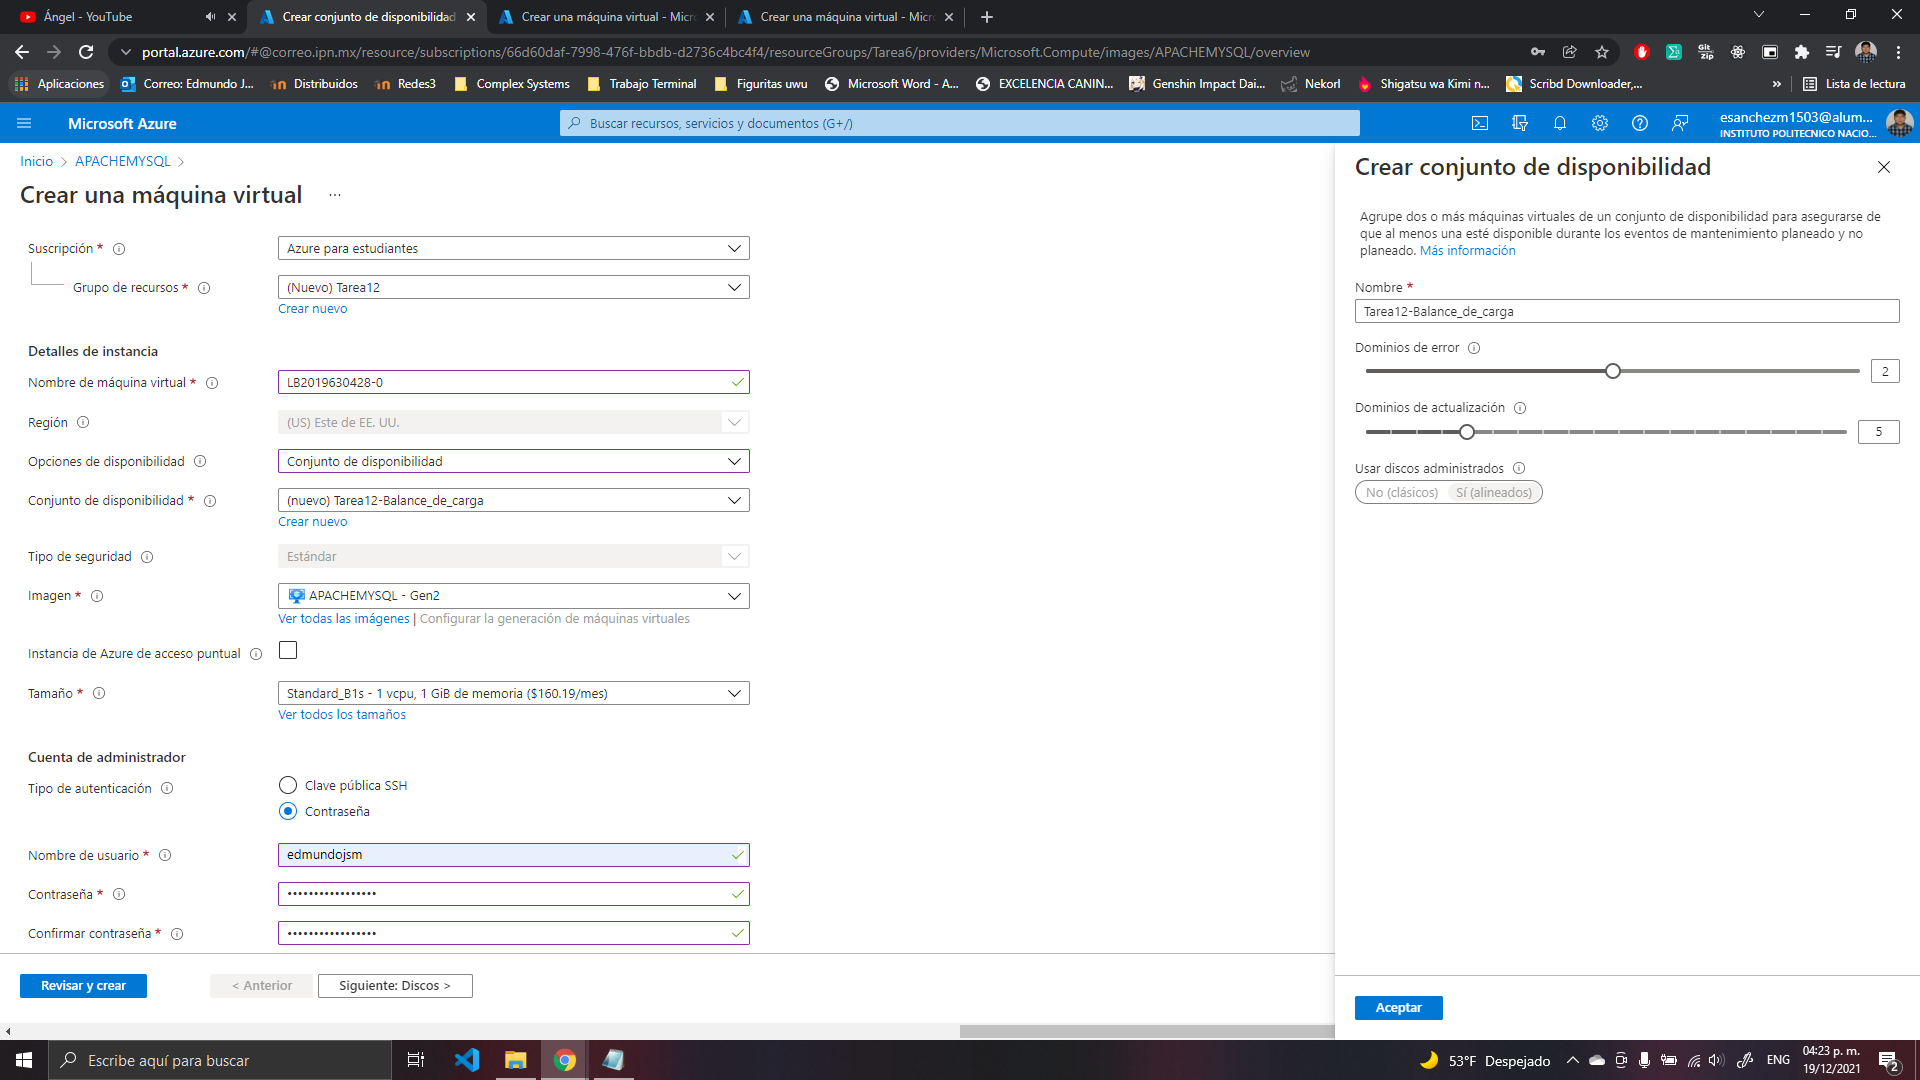
\includegraphics[scale=0.34]{resources/CreacionConjuntoDisponibilidad.png}
			\caption{Creación del conjunto de disponibilidad.}\label{fig:picture}
		\end{figure}
		Ahora si, procedamos a ver la creación de las maquinas virtuales, empezando con el nodo 0.
		\begin{figure}[H]
			\centering
			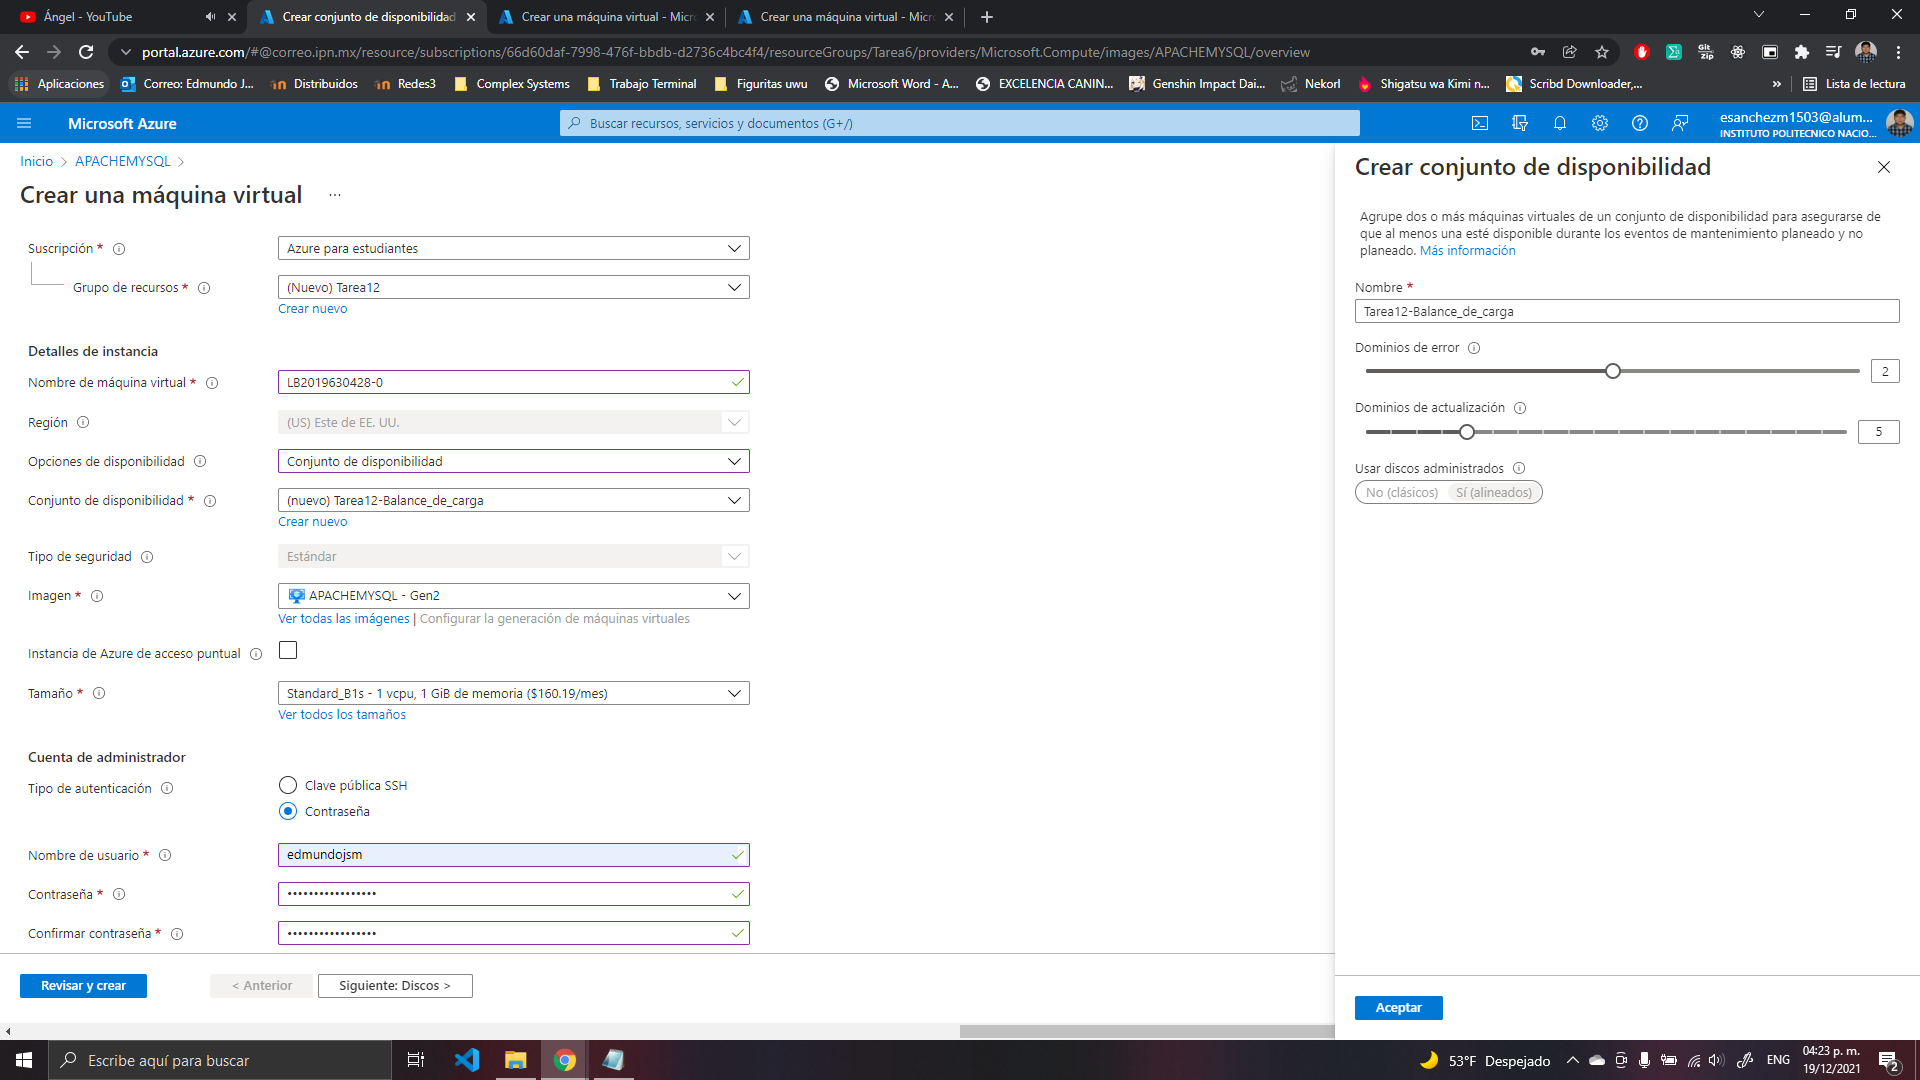
\includegraphics[scale=0.34]{resources/CreacionConjuntoDisponibilidad.png}
			\caption{Datos básicos de la maquina virtual. Nodo 0.}\label{fig:picture}
		\end{figure}
		\begin{figure}[H]
			\centering
			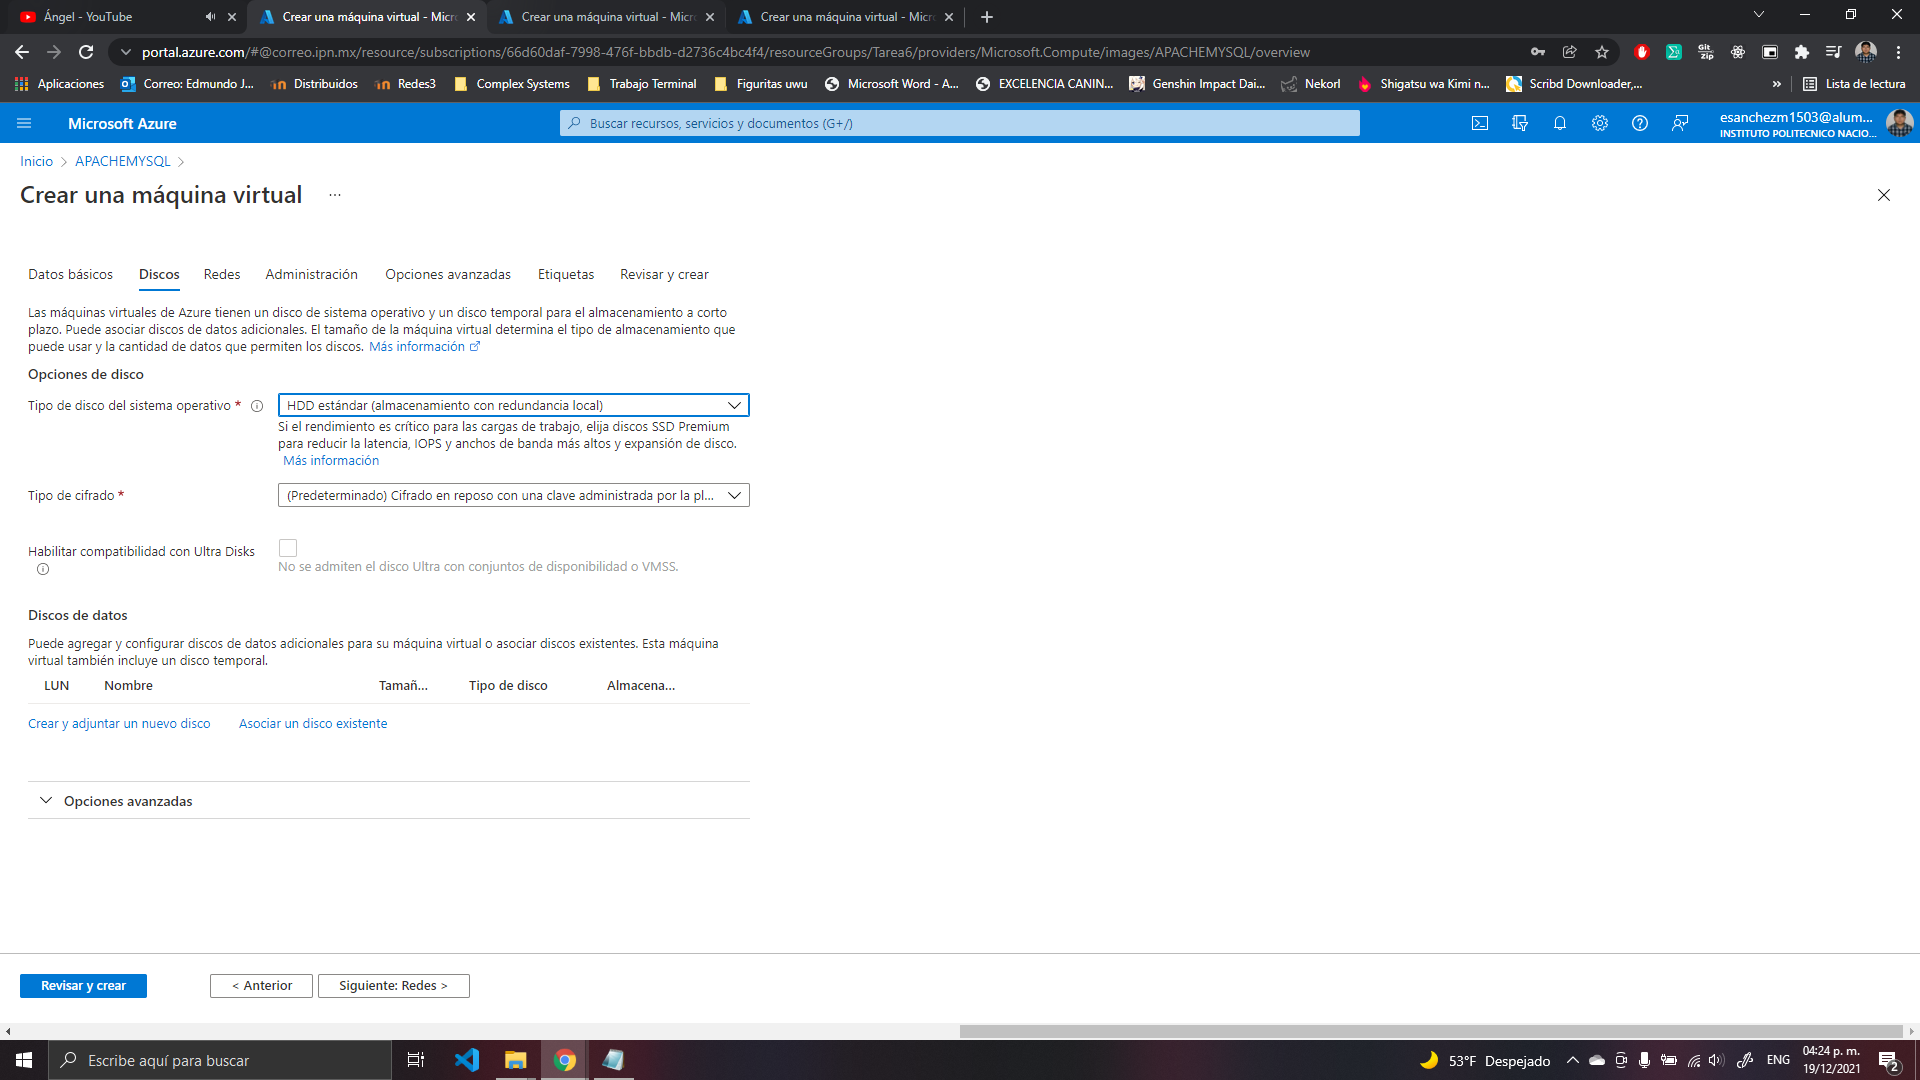
\includegraphics[scale=0.34]{resources/datosdisco0.png}
			\caption{Configuración del tipo de disco de la maquina virtual. Nodo 0.}\label{fig:picture}
		\end{figure}
		\begin{figure}[H]
			\centering
			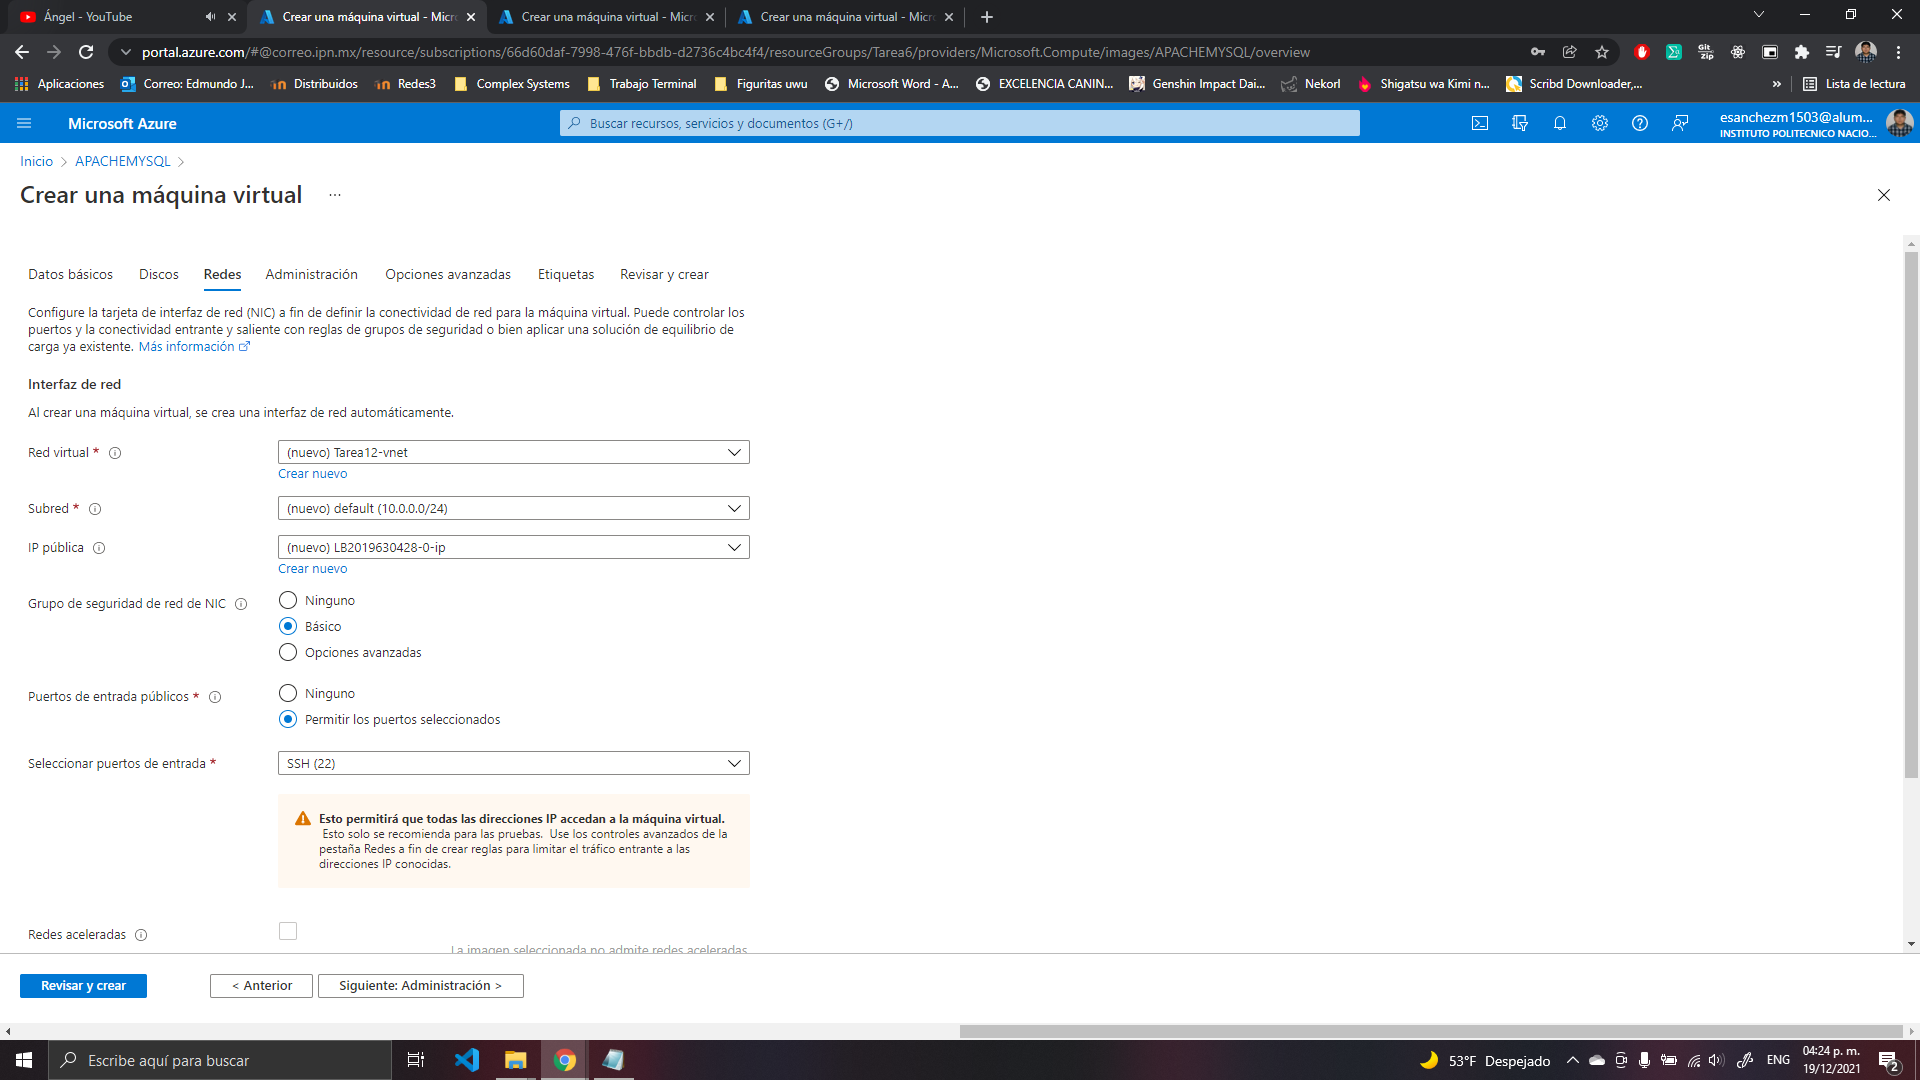
\includegraphics[scale=0.34]{resources/datosredes0.png}
			\caption{Información sobre la redes de la maquina virtual. Nodo 0.}\label{fig:picture}
		\end{figure}
		\begin{figure}[H]
			\centering
			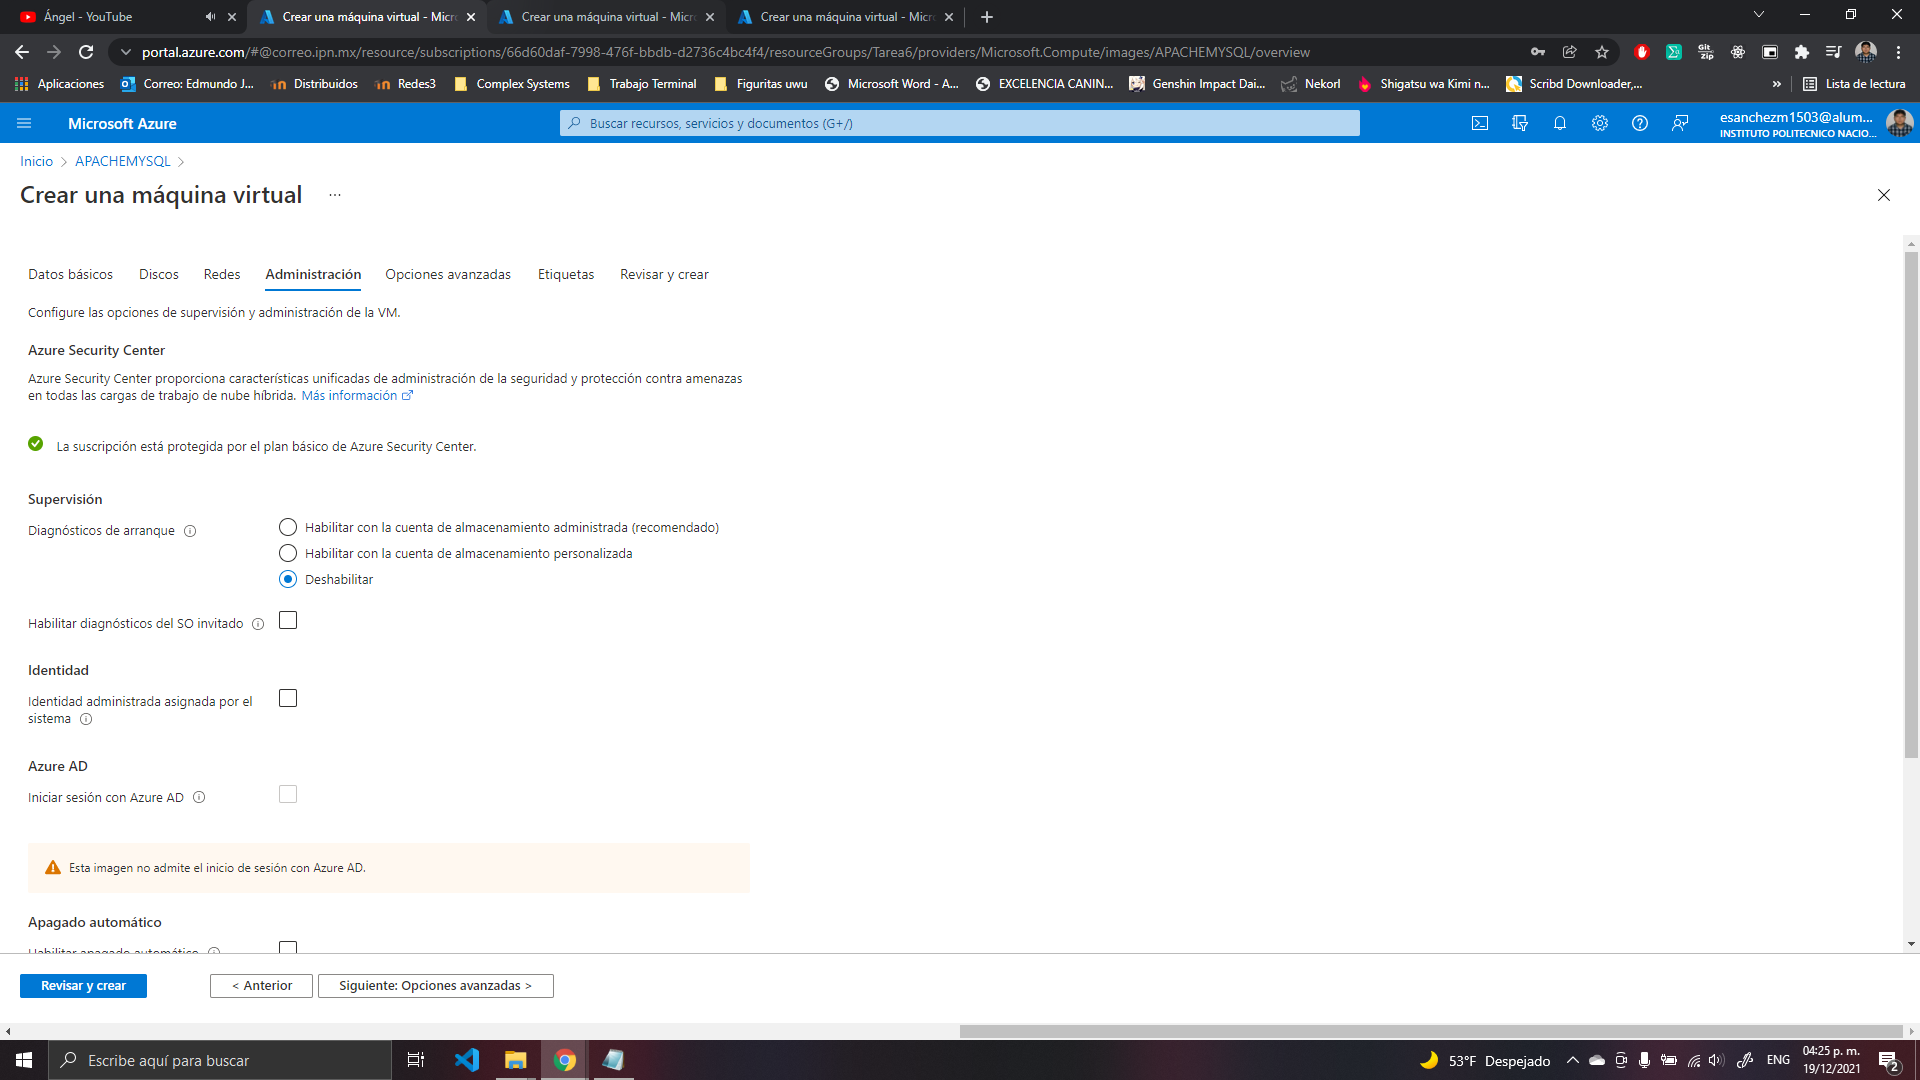
\includegraphics[scale=0.34]{resources/datosadministracion0.png}
			\caption{Configuración de la administración de la maquina virtual. Nodo 0.}\label{fig:picture}
		\end{figure}
		\begin{figure}[H]
			\centering
			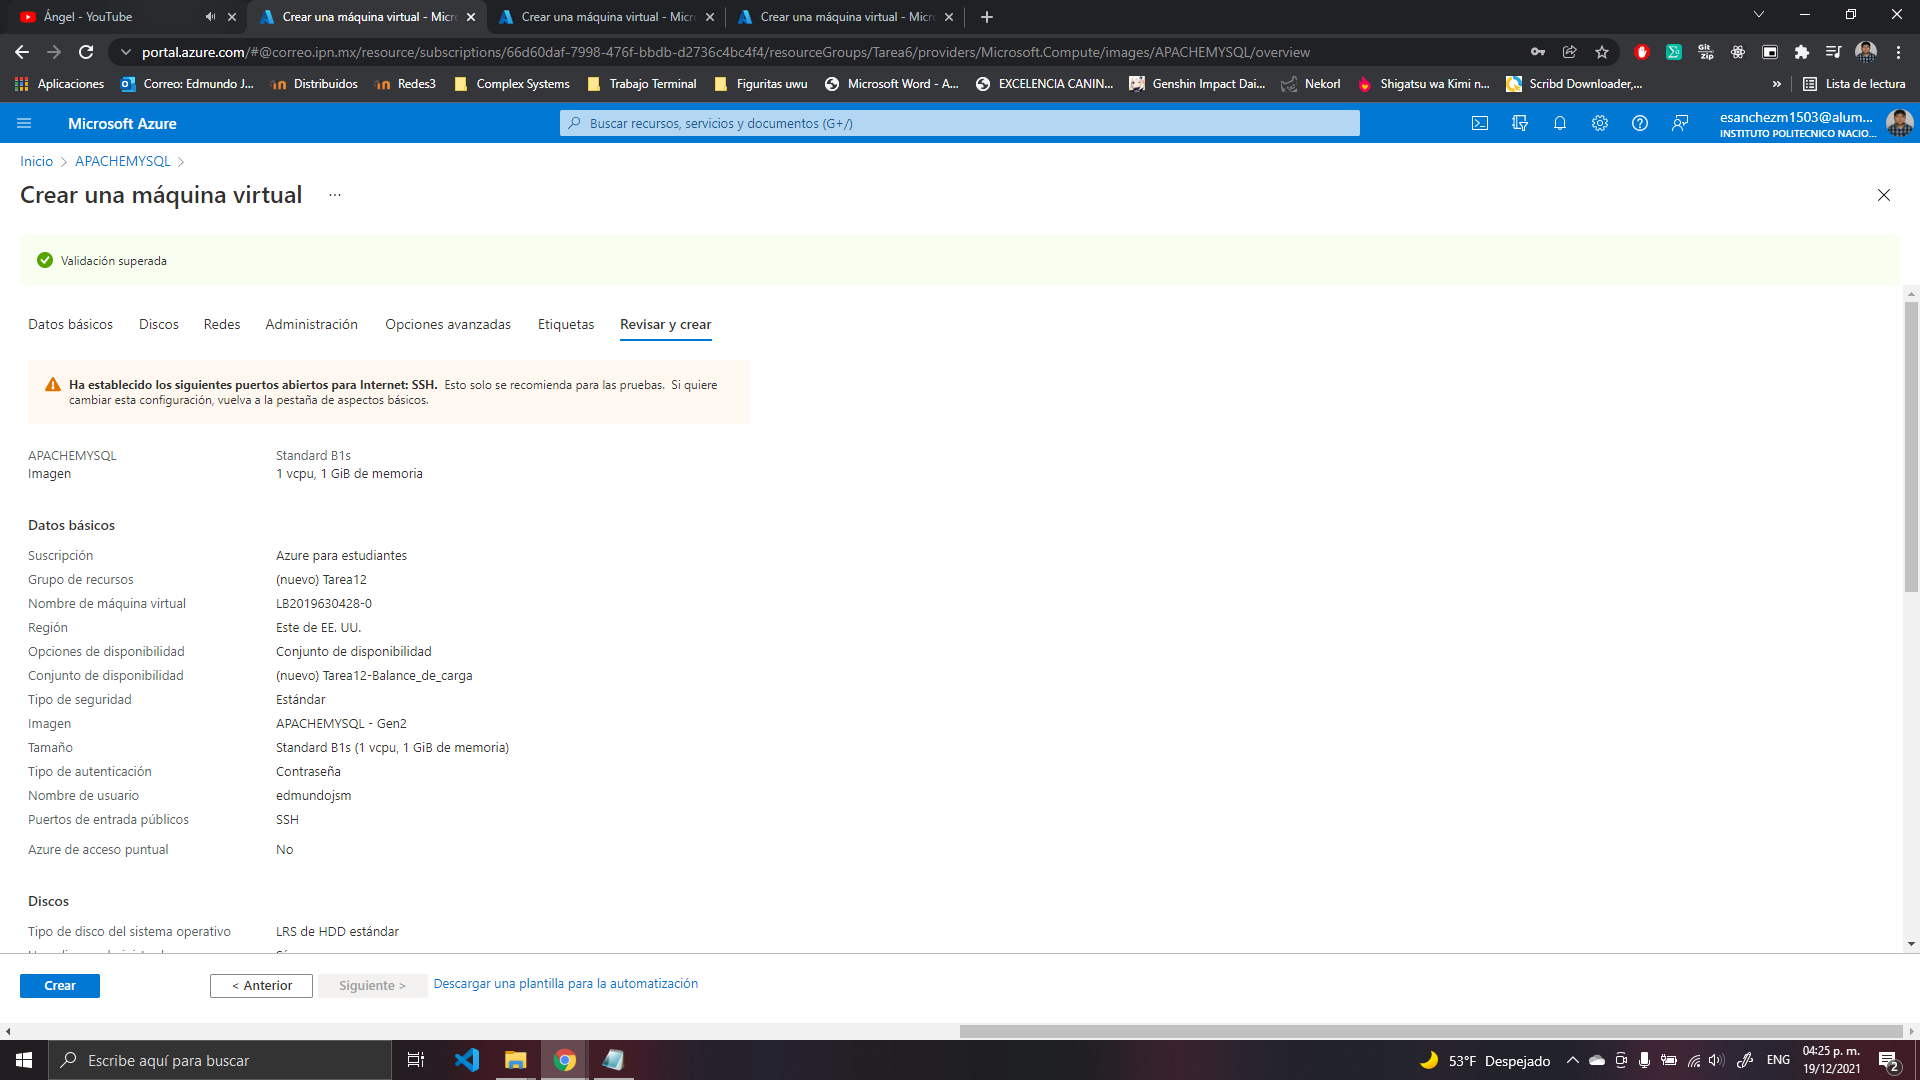
\includegraphics[scale=0.34]{resources/revisarycrear0.png}
			\caption{Creación de la maquina virtual. Nodo 0.}\label{fig:picture}
		\end{figure}
		\begin{figure}[H]
			\centering
			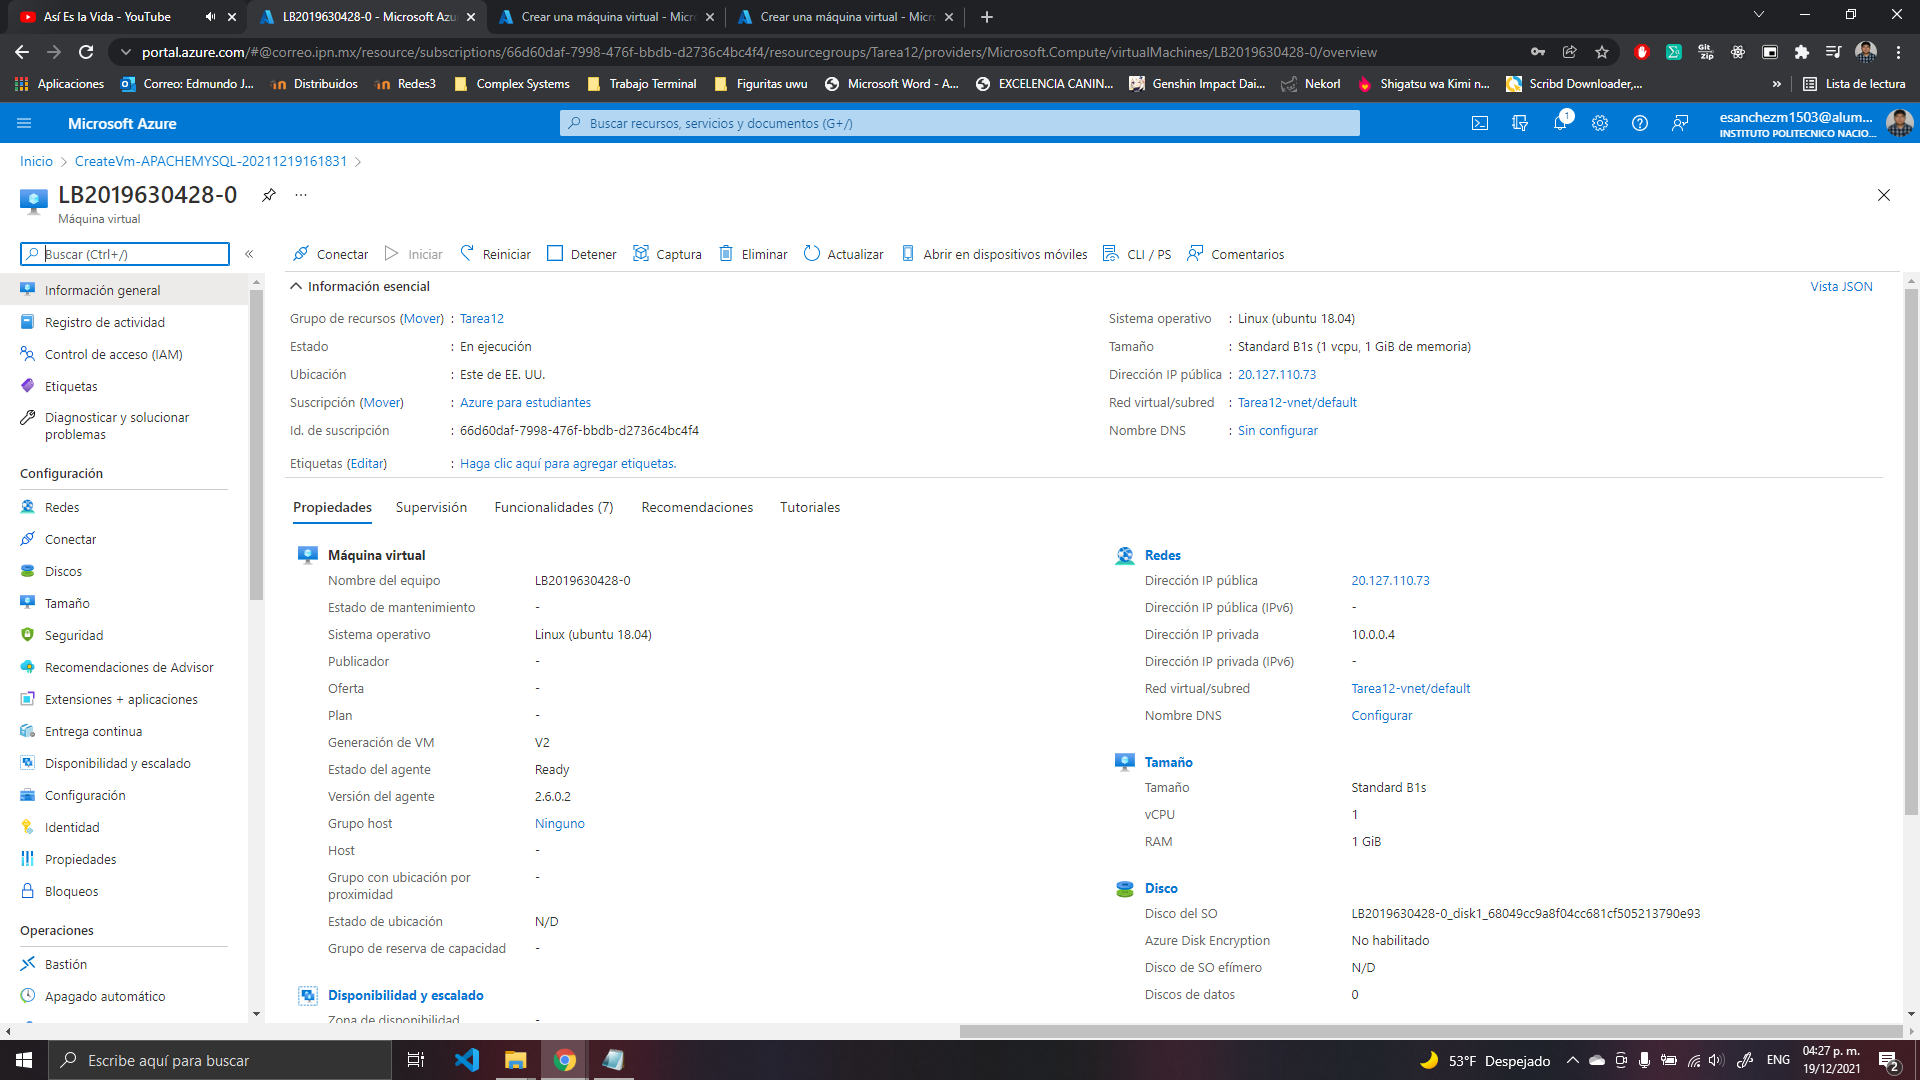
\includegraphics[scale=0.34]{resources/Panelcontrol0.png}
			\caption{Panel de control de la maquina virtual. Nodo 0.}\label{fig:picture}
		\end{figure}
		Ahora veamos la creación de la maquina virtual para el nodo 1
		\begin{figure}[H]
			\centering
			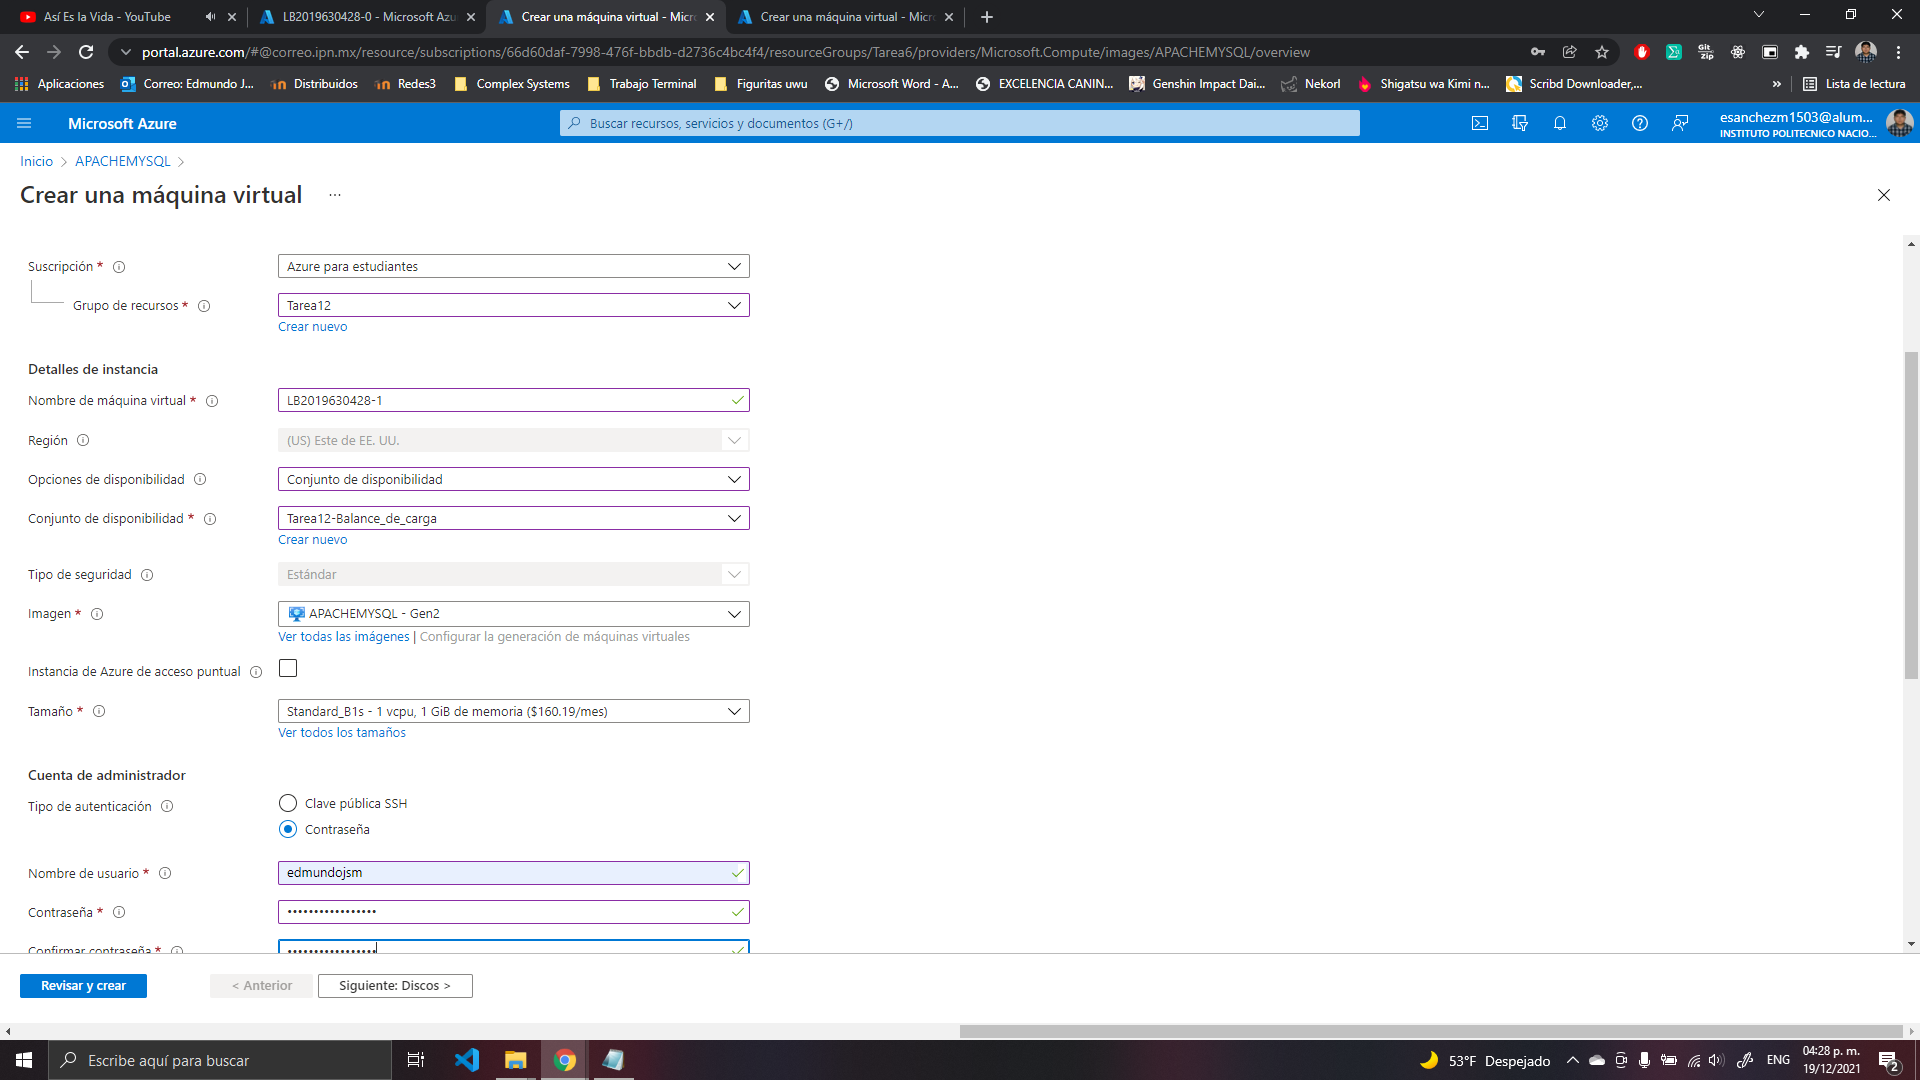
\includegraphics[scale=0.34]{resources/datosbasicos1.png}
			\caption{Datos básicos de la maquina virtual. Nodo 1.}\label{fig:picture}
		\end{figure}
		\begin{figure}[H]
			\centering
			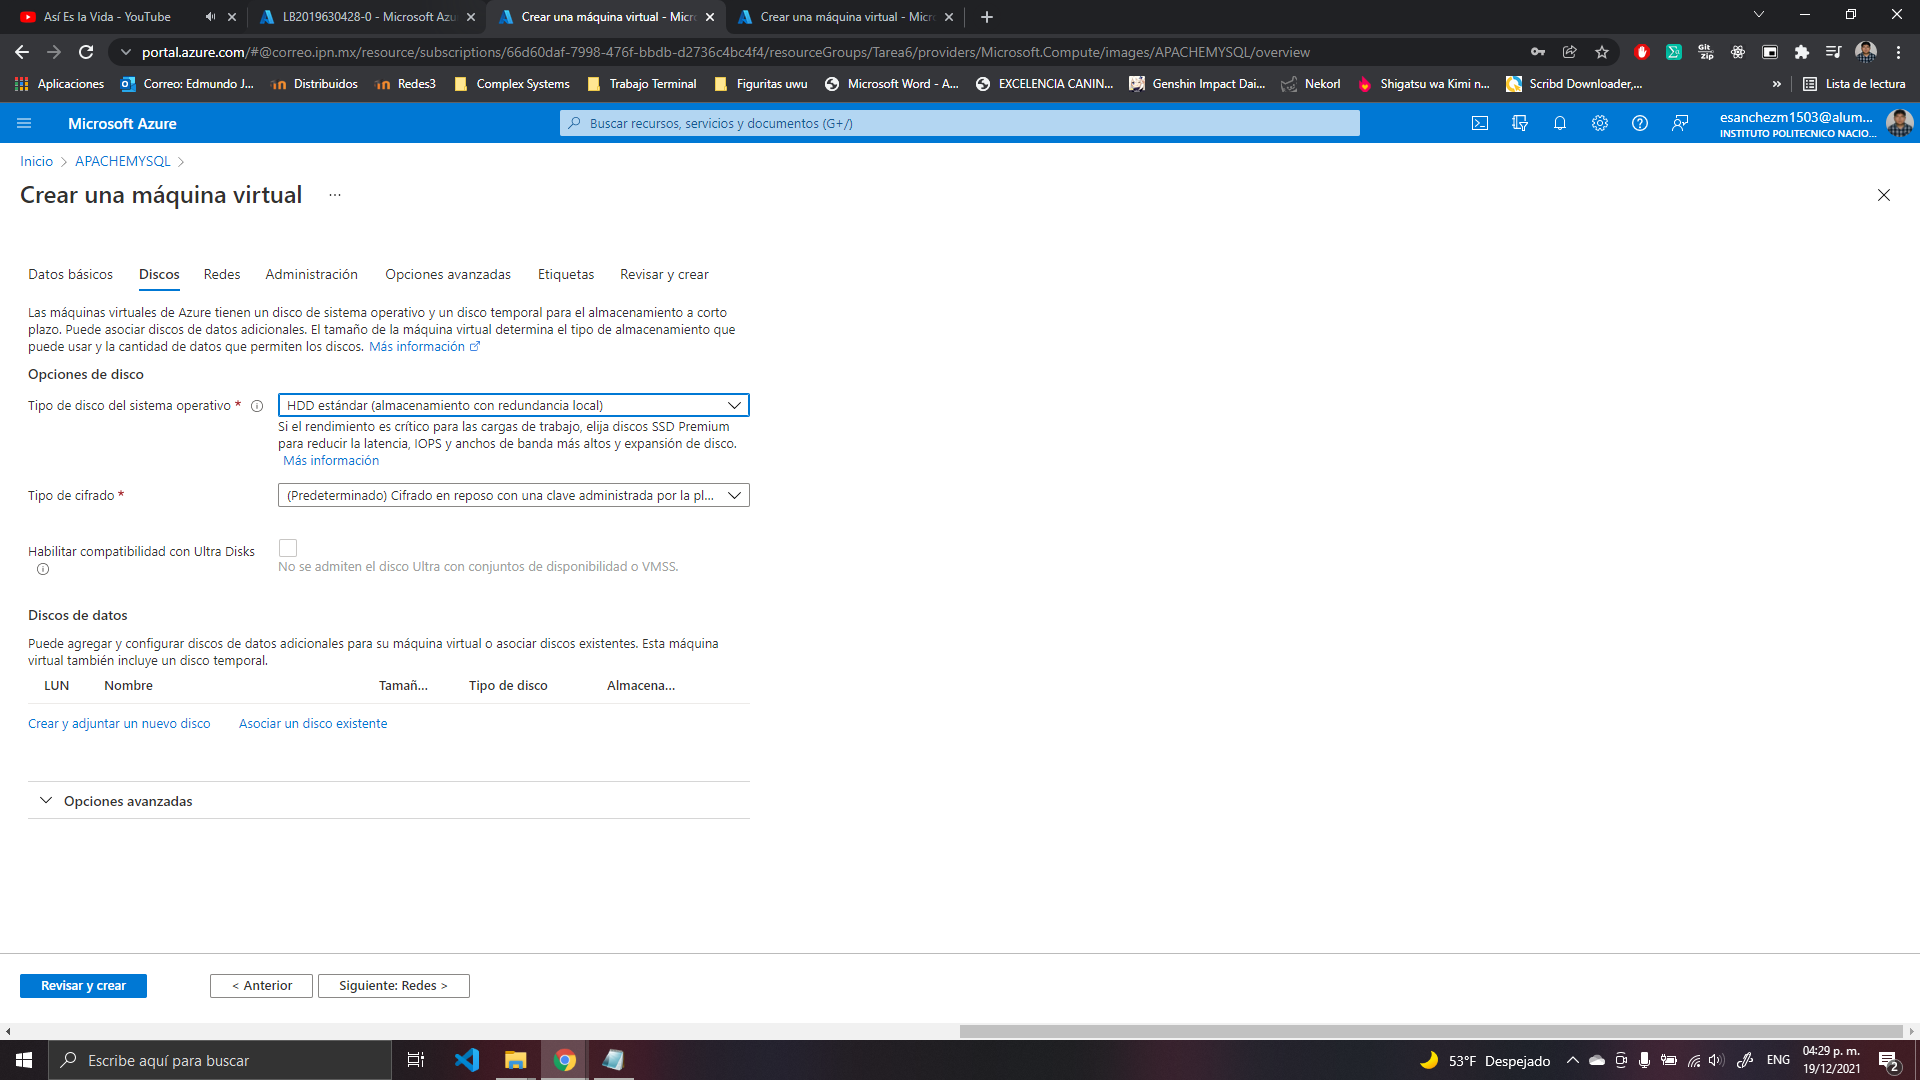
\includegraphics[scale=0.34]{resources/datosdisco1.png}
			\caption{Configuración del tipo de disco de la maquina virtual. Nodo 1.}\label{fig:picture}
		\end{figure}
		\begin{figure}[H]
			\centering
			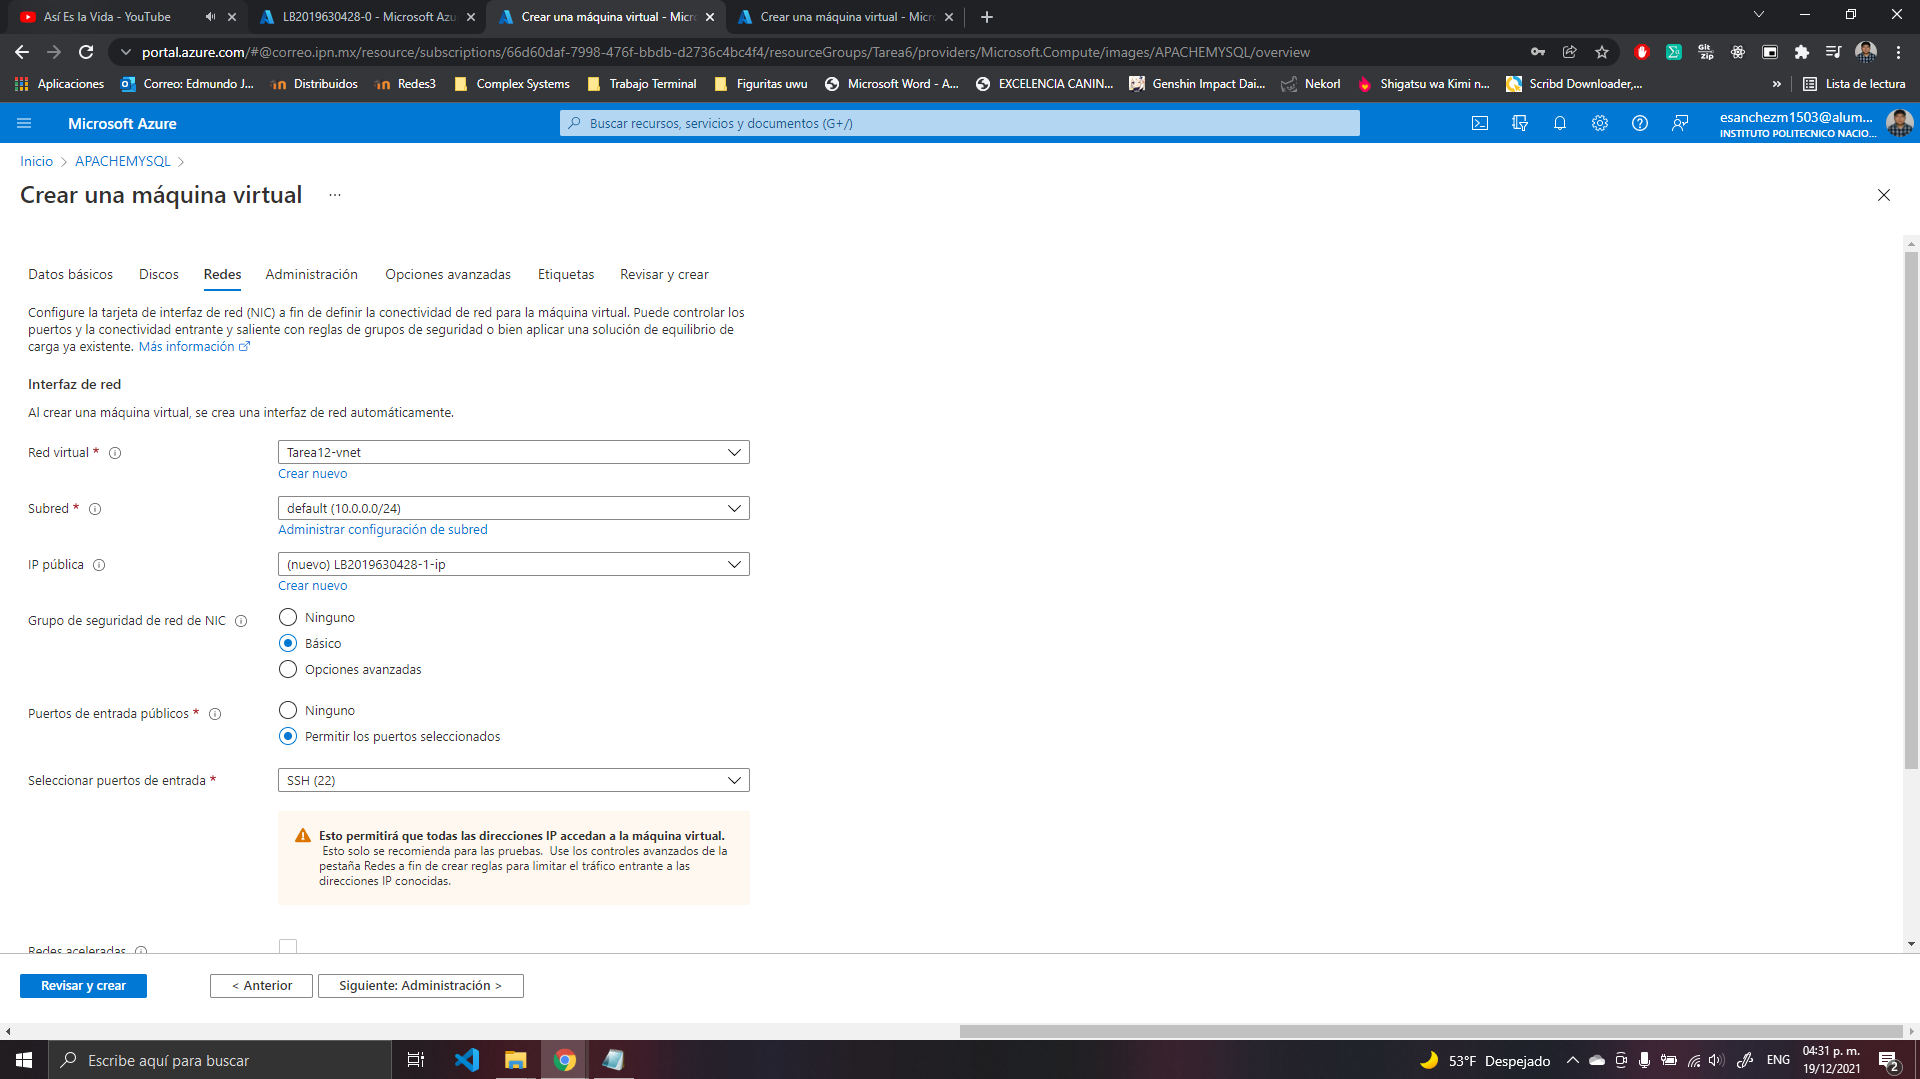
\includegraphics[scale=0.34]{resources/datosredes1.png}
			\caption{Información sobre la redes de la maquina virtual. Nodo 1.}\label{fig:picture}
		\end{figure}
		\begin{figure}[H]
			\centering
			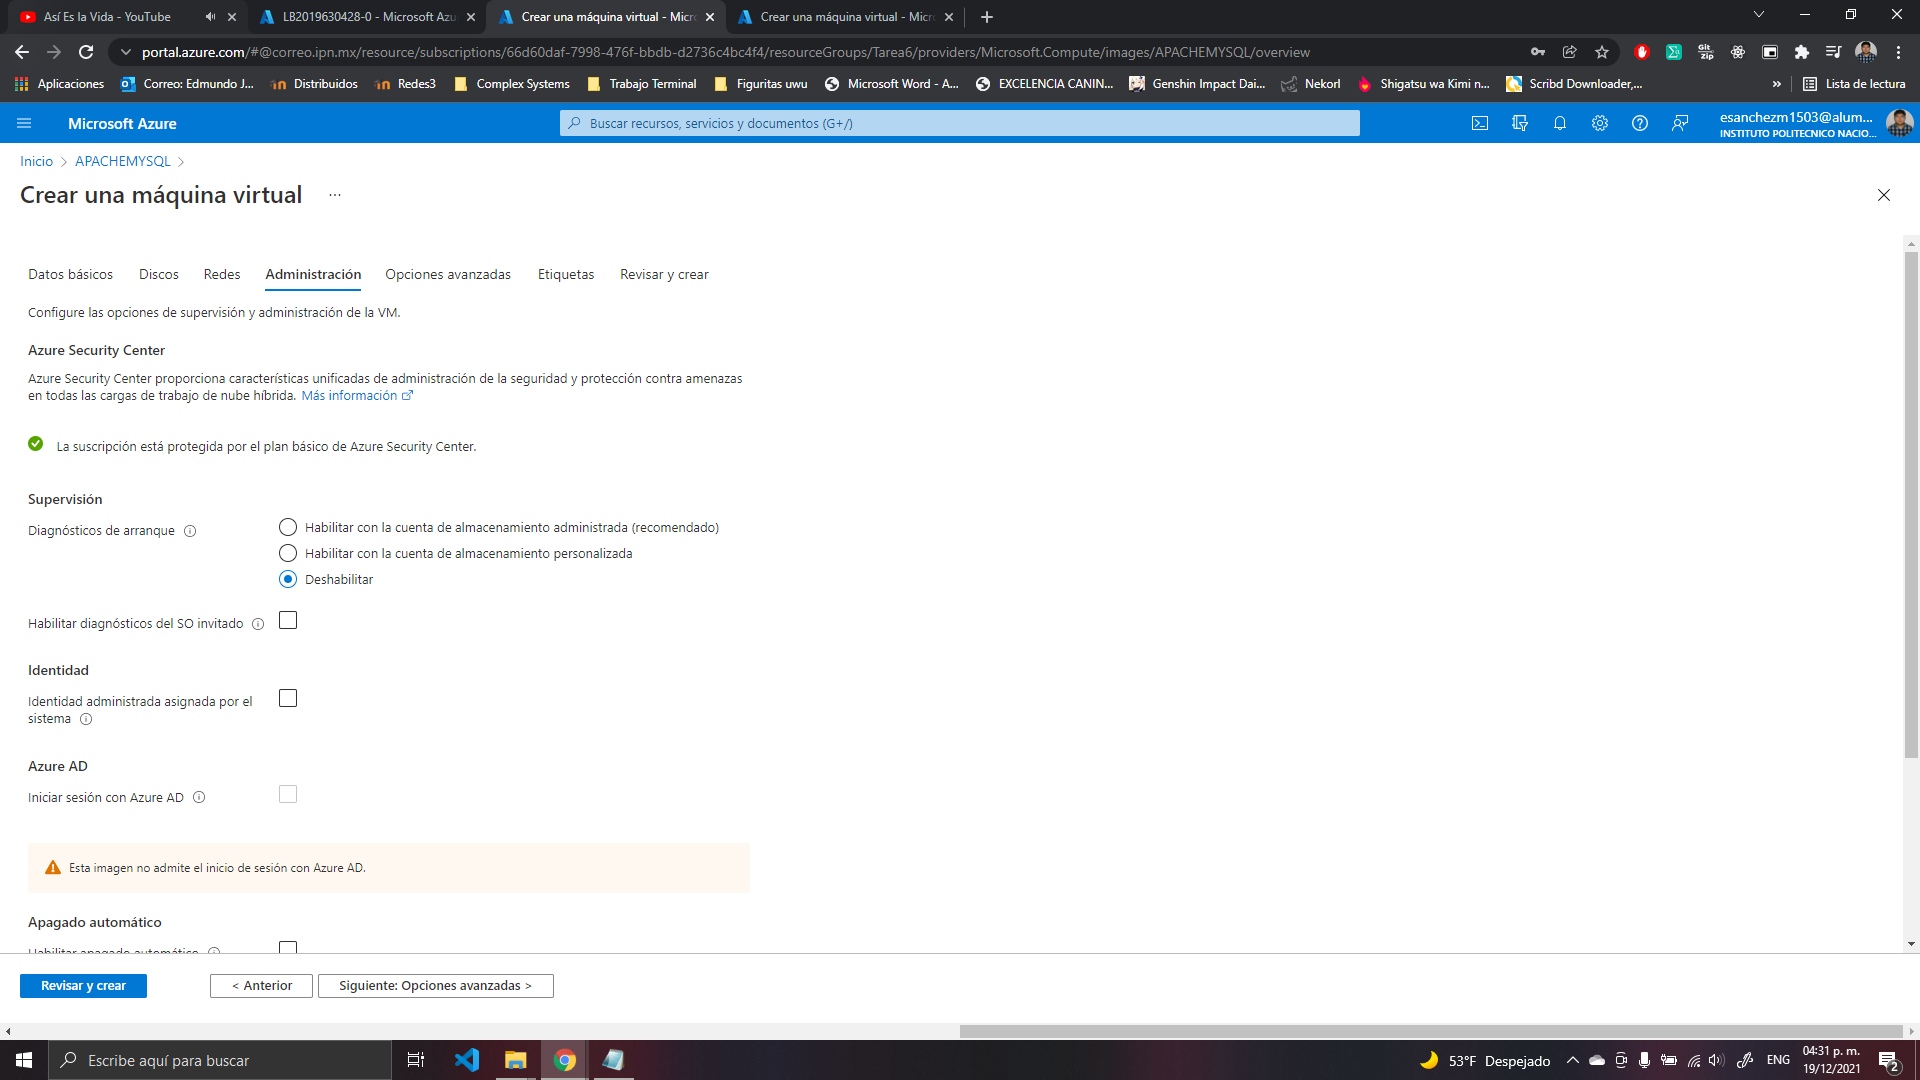
\includegraphics[scale=0.34]{resources/datosadministracion1.png}
			\caption{Configuración de la administración de la maquina virtual. Nodo 1.}\label{fig:picture}
		\end{figure}
		\begin{figure}[H]
			\centering
			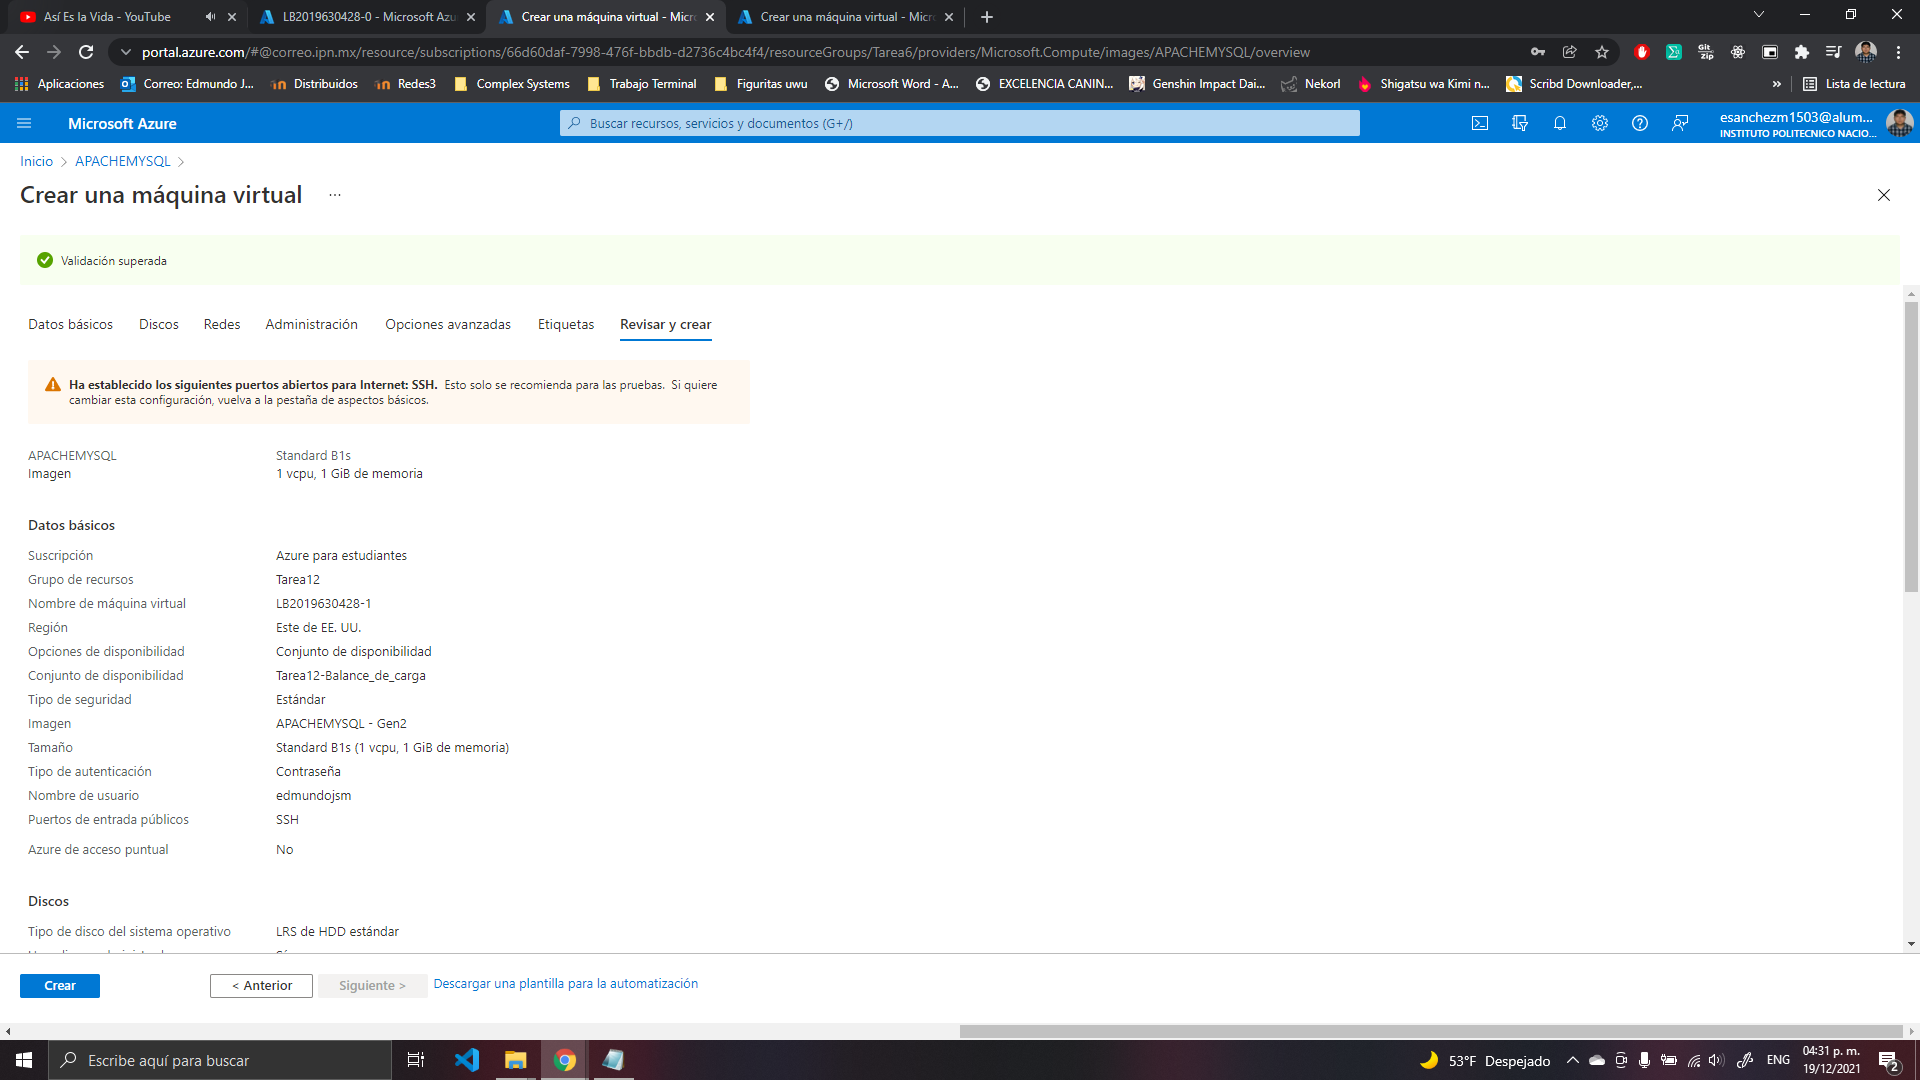
\includegraphics[scale=0.34]{resources/revisarycrear1.png}
			\caption{Creación de la maquina virtual. Nodo 1.}\label{fig:picture}
		\end{figure}
		\begin{figure}[H]
			\centering
			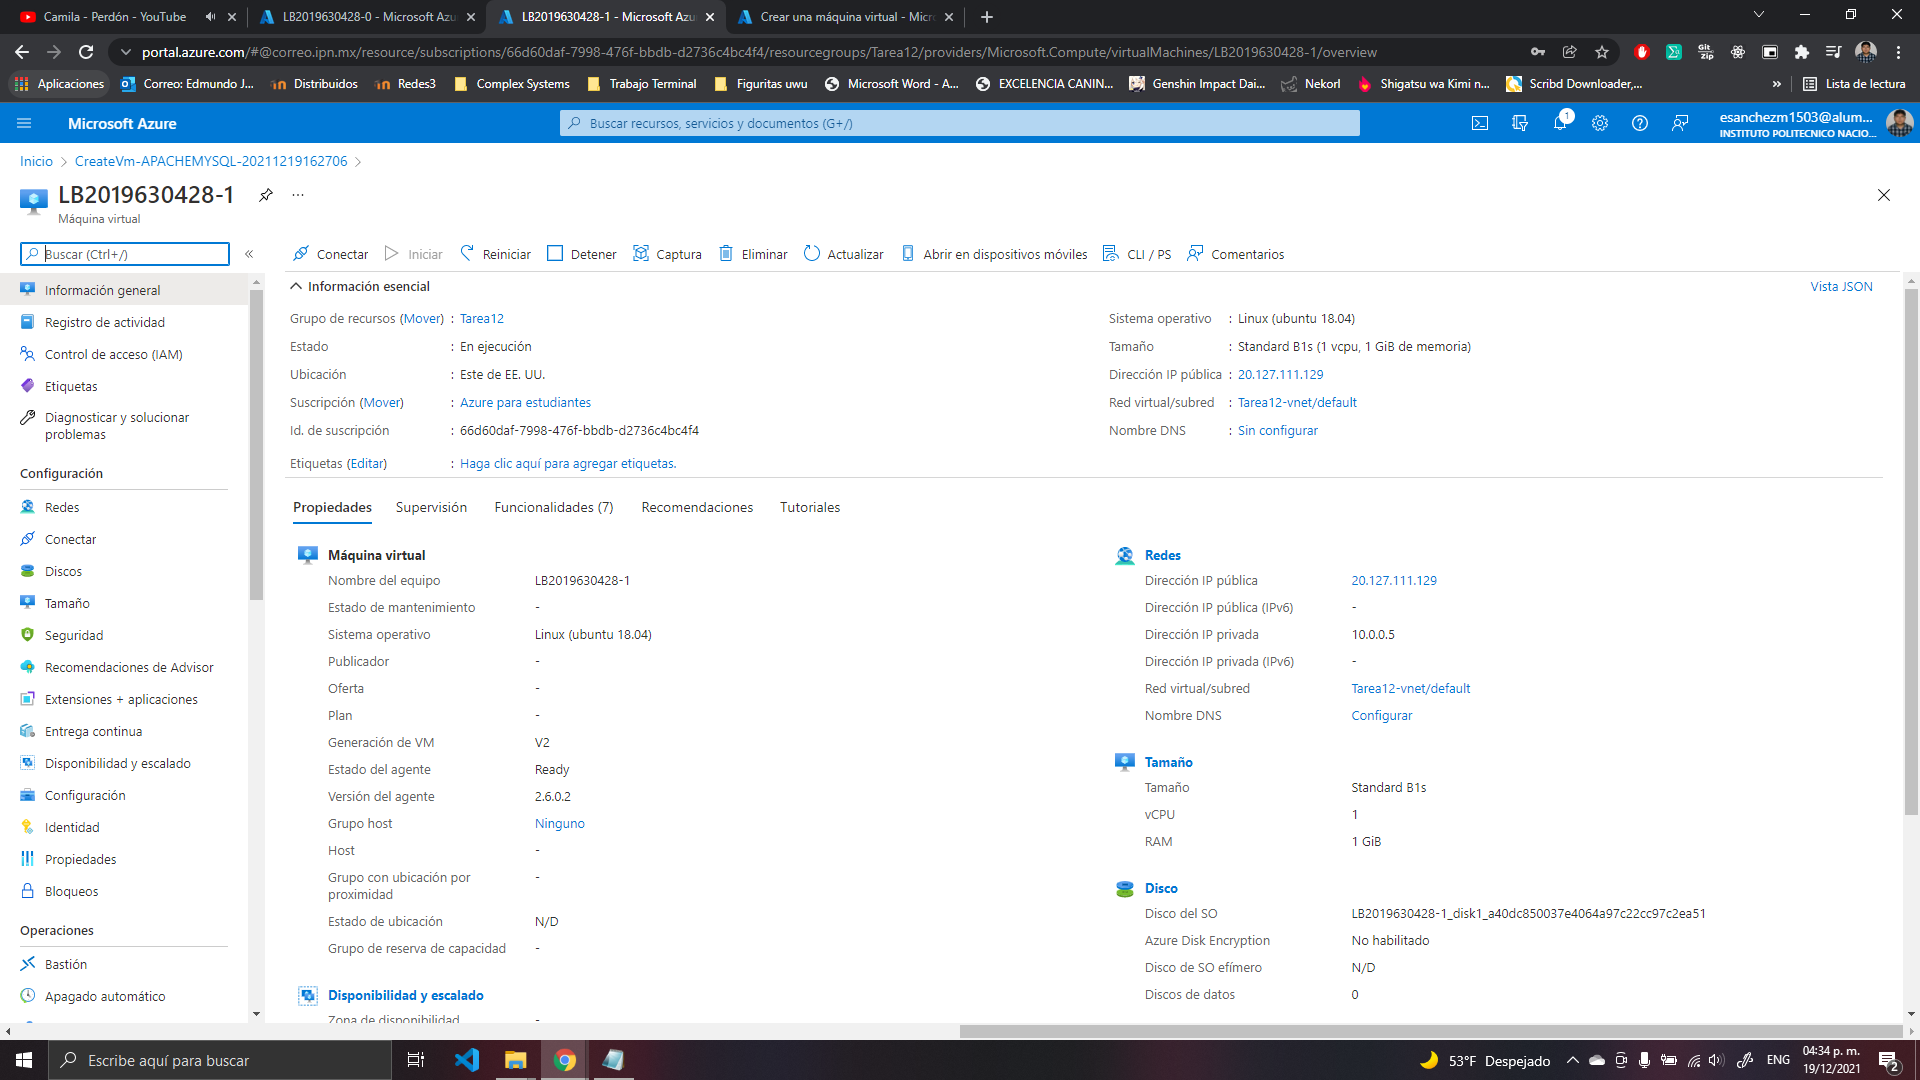
\includegraphics[scale=0.34]{resources/Panelcontrol1.png}
			\caption{Panel de control de la maquina virtual. Nodo 1.}\label{fig:picture}
		\end{figure}
		
		\subsection{Creación de la maquina virtual (nodo 3) y creación la base de datos ``servicio\_web'' y el usuario ``hugo'' en MySQL}
		En esta parte veremos la creación de la maquina virtual que se ocupara para tener MYSQL, por lo que tendrá la base de datos ``servicio\_web'' y el usuario ``hugo'' en MYSQL, mencionar que como estamos tomando como base la imagen creada en la tarea 6 de este curso, ya no es necesario la creación de estos dos, pero si es necesario la actualización del usuario hugo para que sea usable para conexión remota en MYSQL.
		\begin{figure}[H]
			\centering
			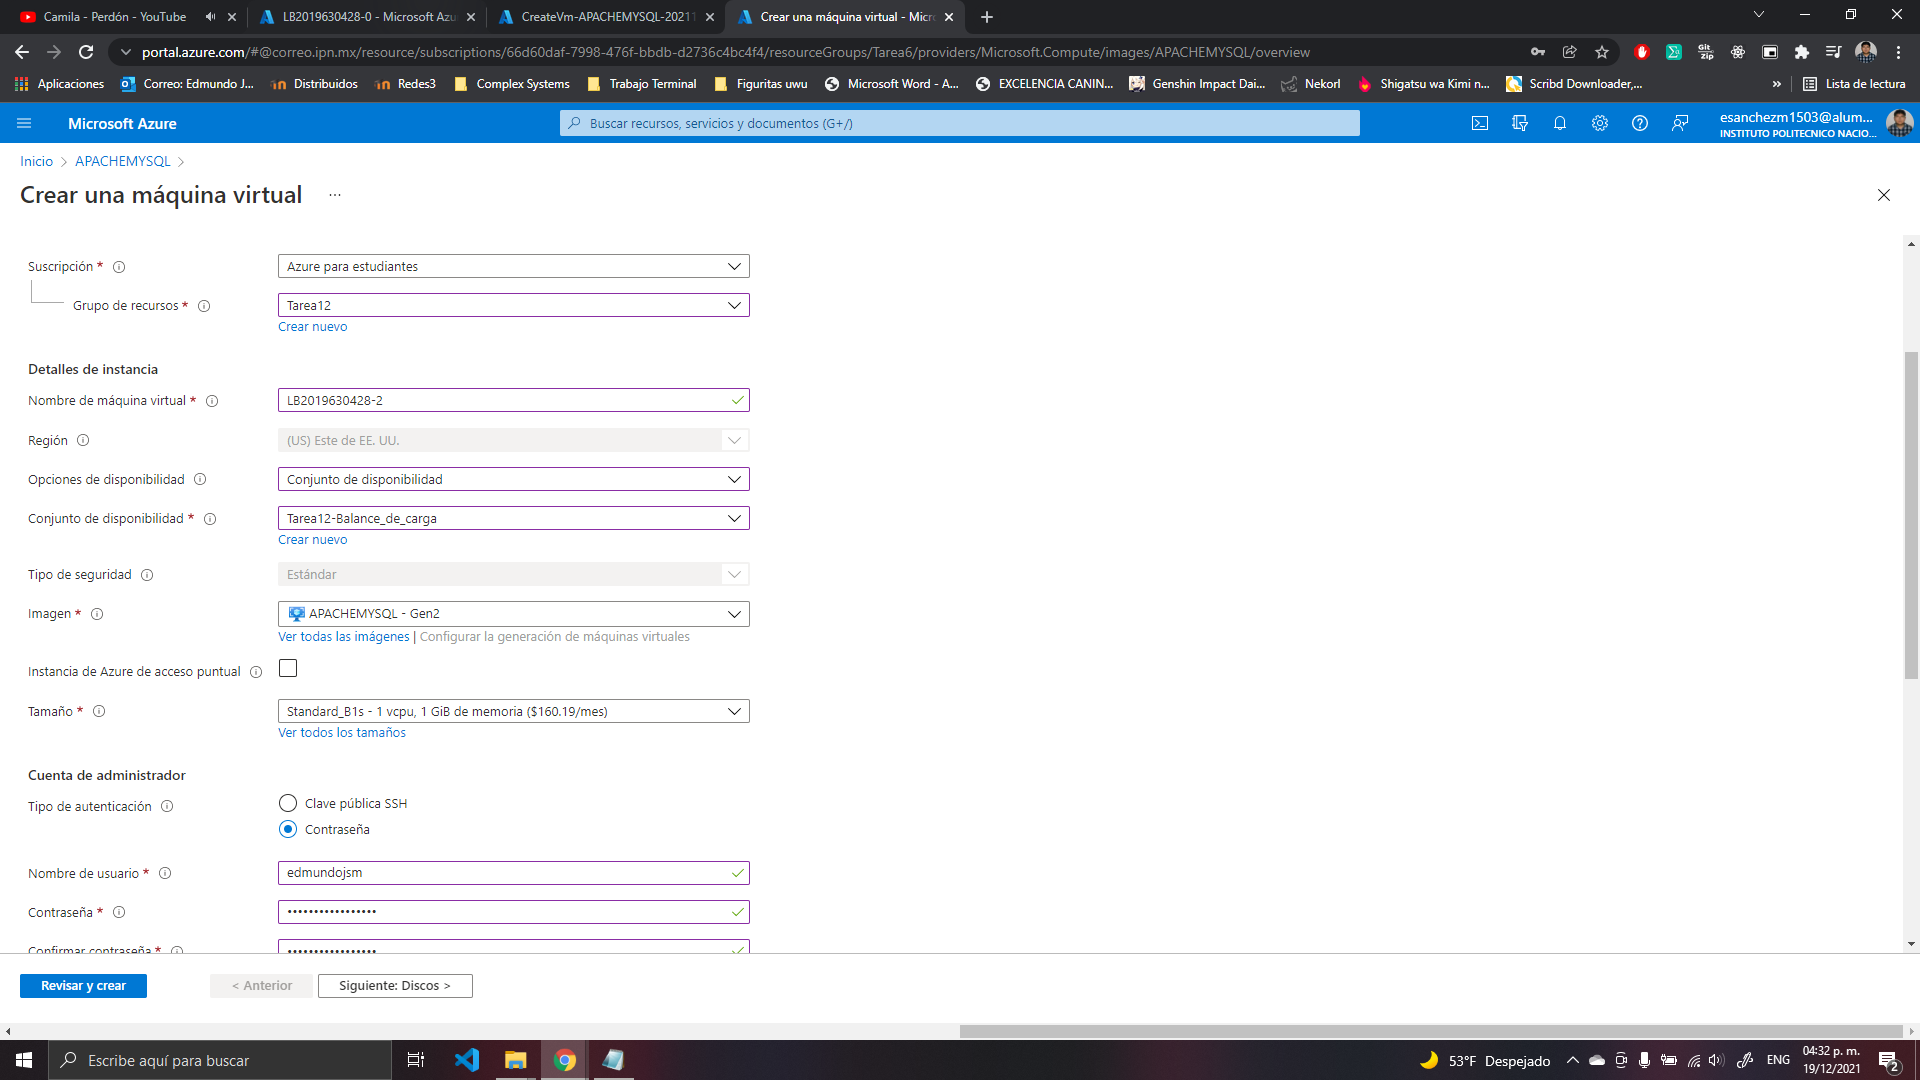
\includegraphics[scale=0.34]{resources/datosbasicos2.png}
			\caption{Datos básicos de la maquina virtual. Nodo 2.}\label{fig:picture}
		\end{figure}
		\begin{figure}[H]
			\centering
			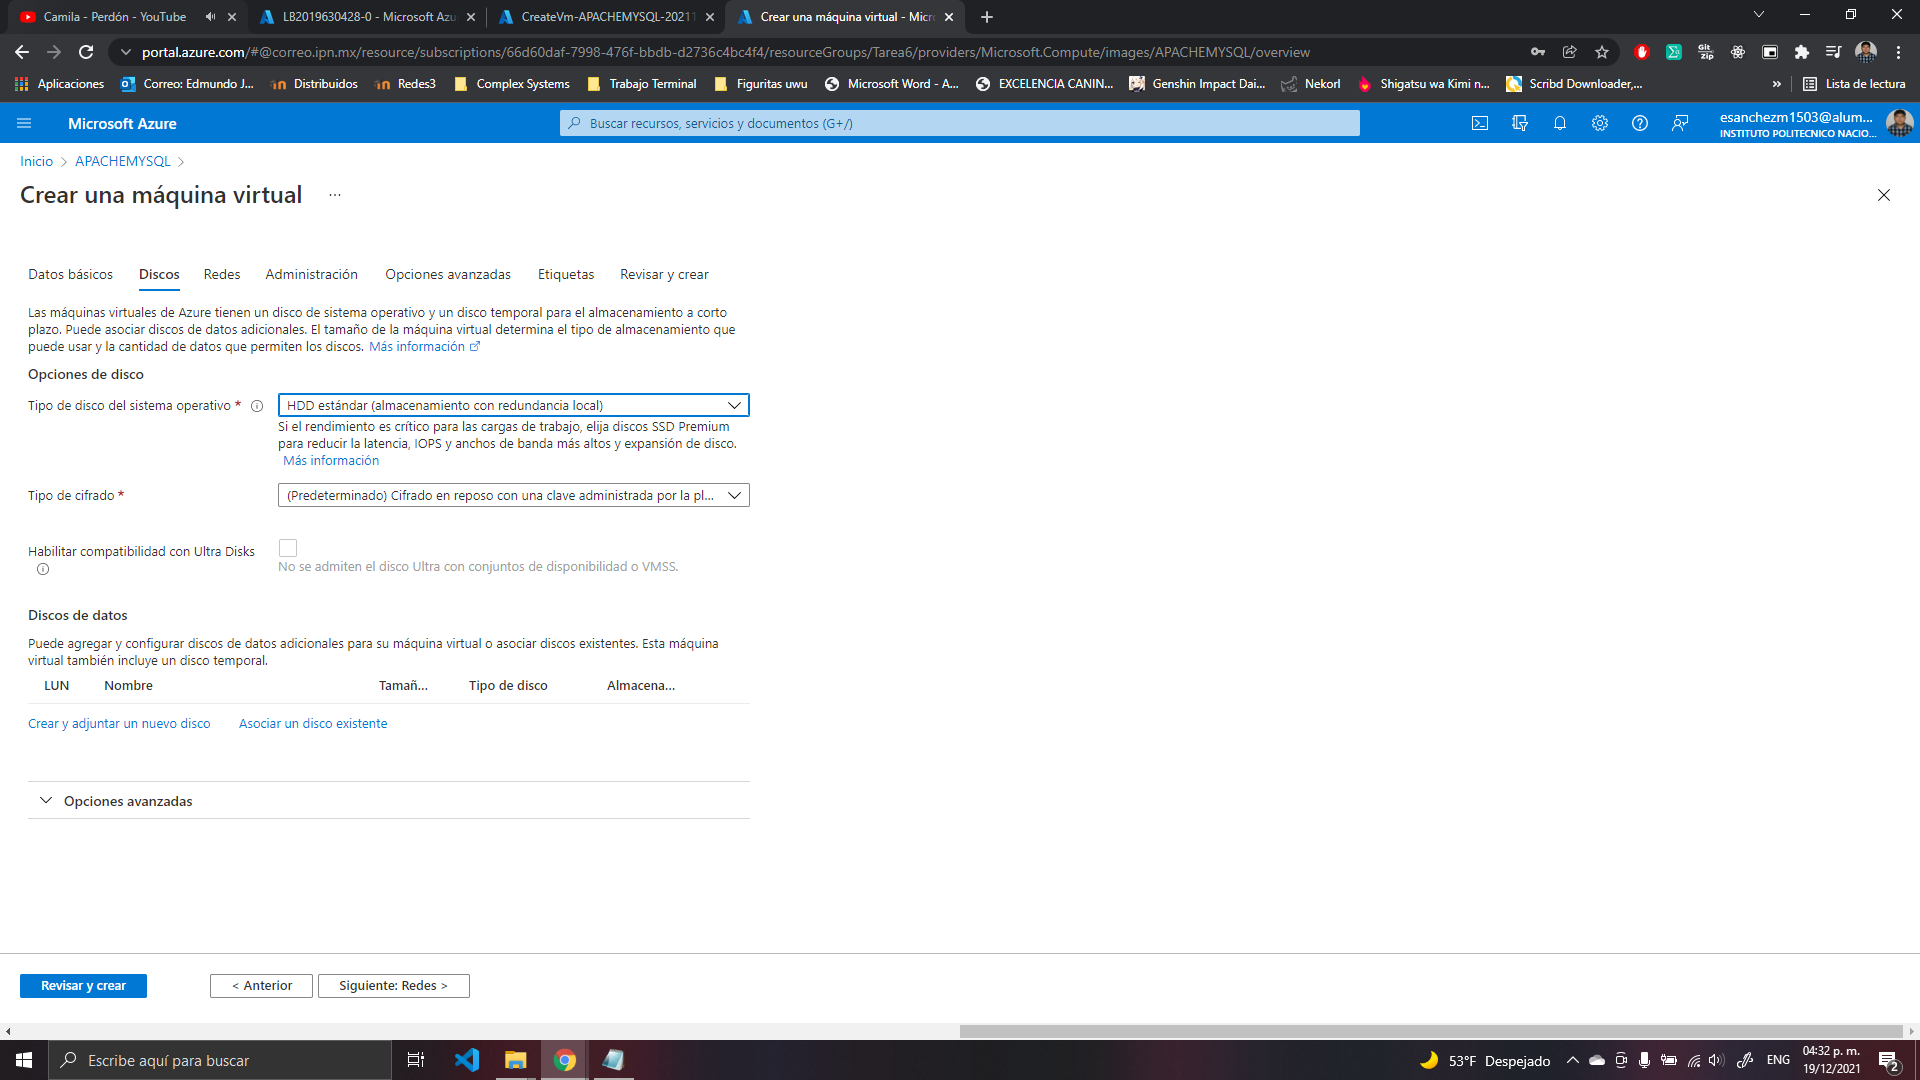
\includegraphics[scale=0.34]{resources/datosdisco2.png}
			\caption{Configuración del tipo de disco de la maquina virtual. Nodo 2.}\label{fig:picture}
		\end{figure}
		\begin{figure}[H]
			\centering
			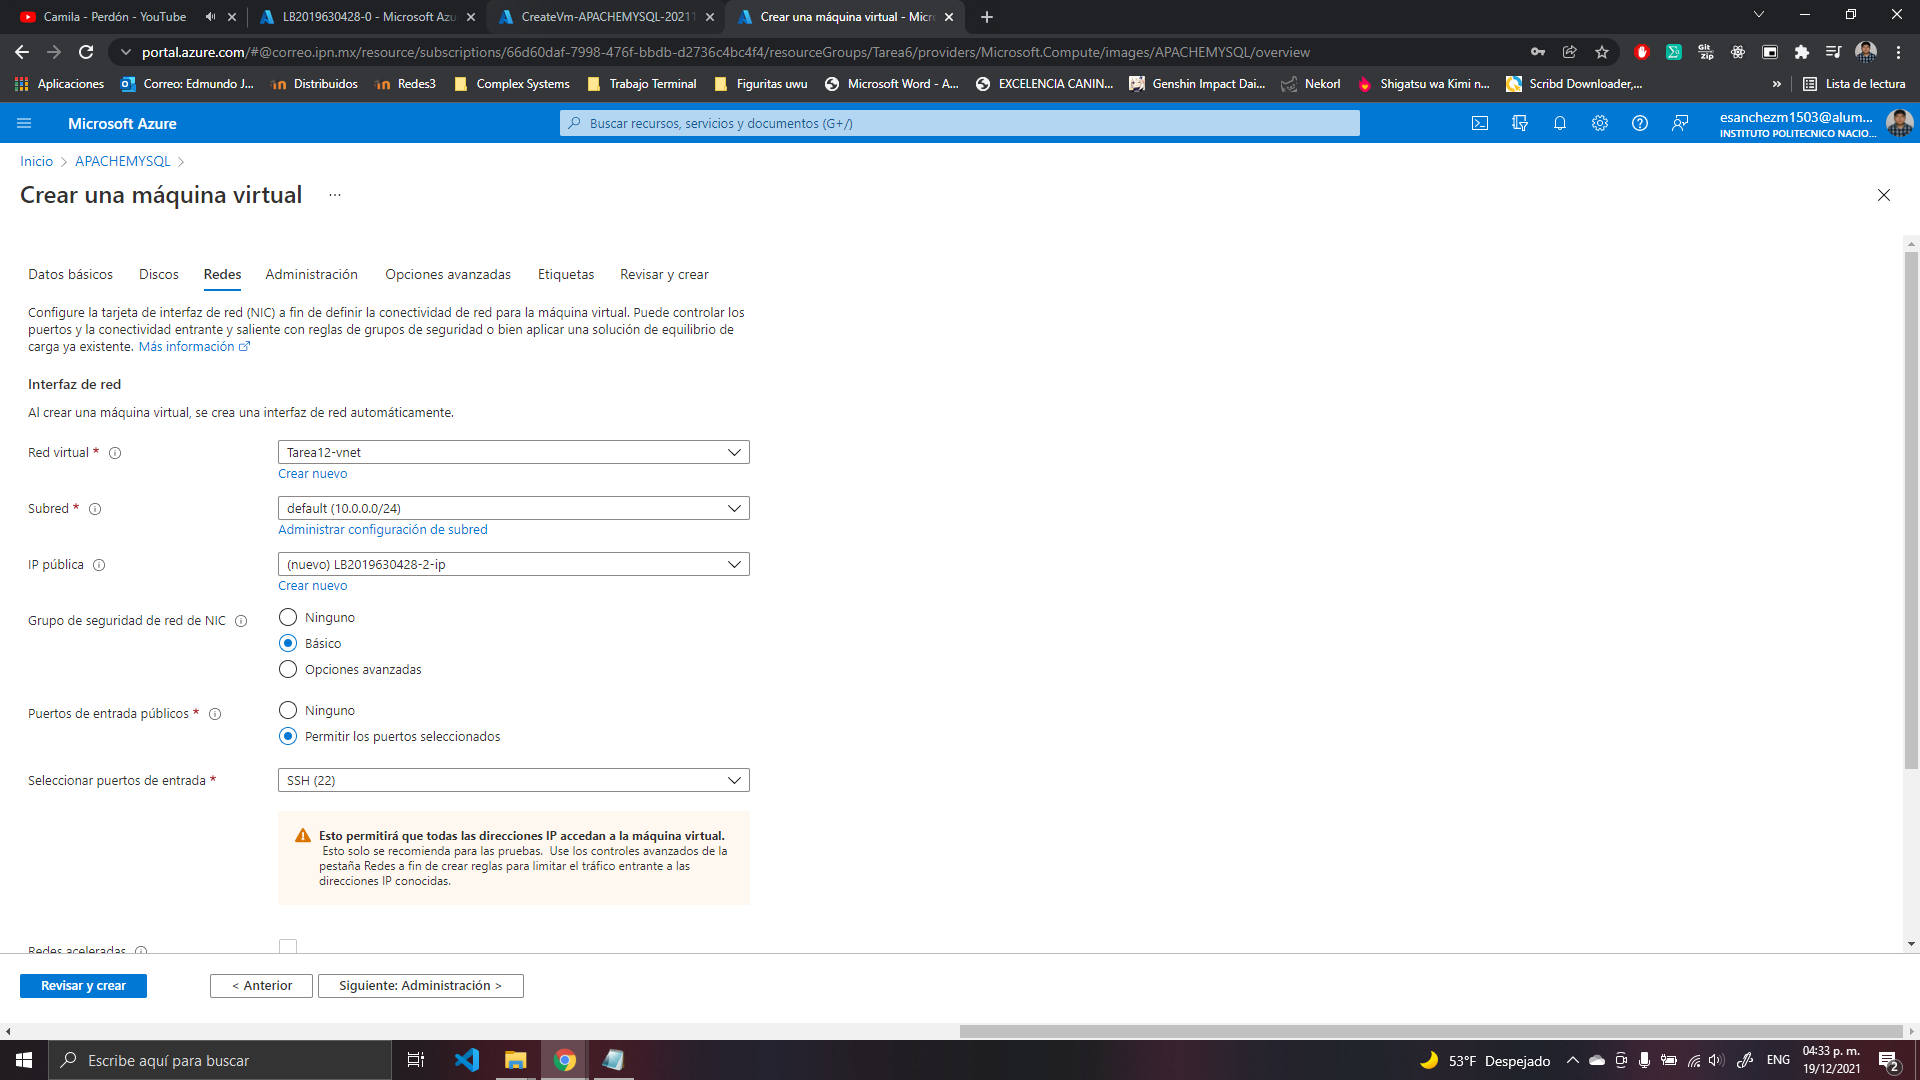
\includegraphics[scale=0.34]{resources/datosredes2.png}
			\caption{Información sobre la redes de la maquina virtual. Nodo 2.}\label{fig:picture}
		\end{figure}
		\begin{figure}[H]
			\centering
			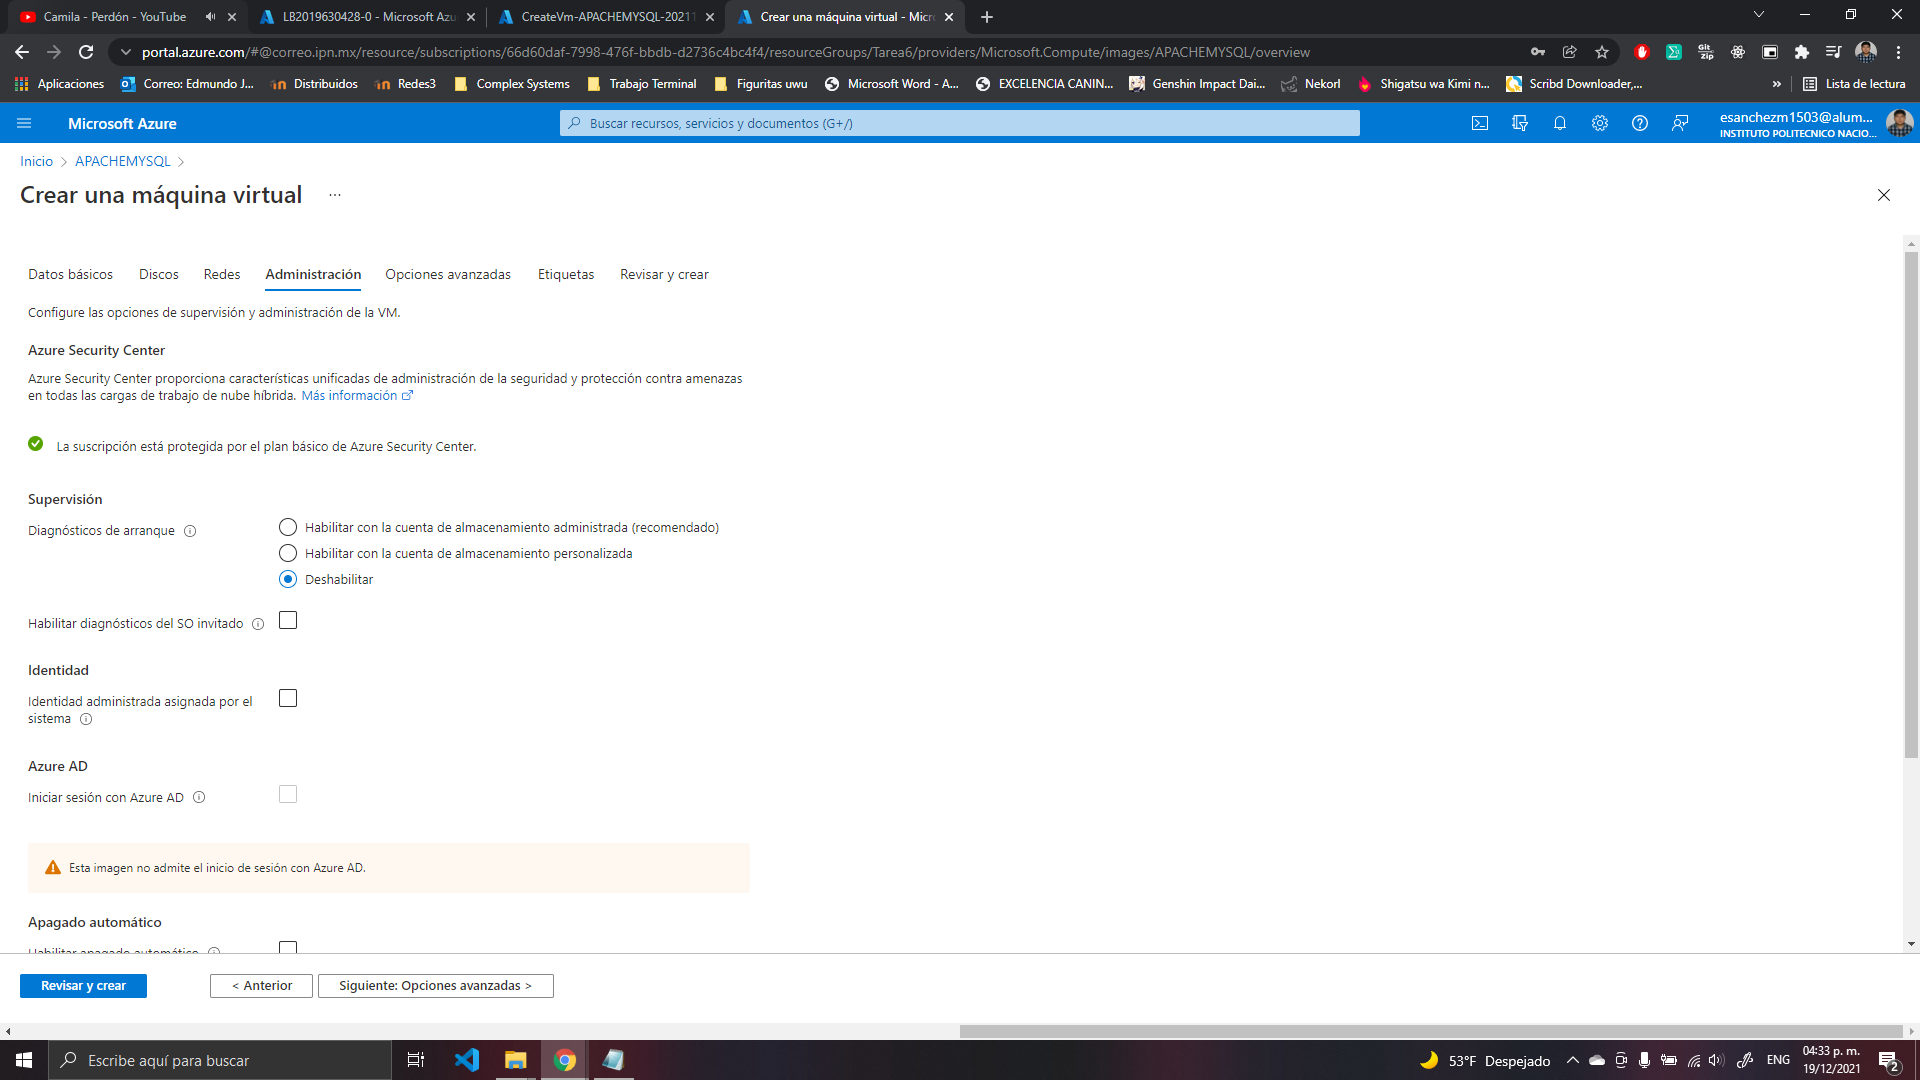
\includegraphics[scale=0.34]{resources/datosadministracion2.png}
			\caption{Configuración de la administración de la maquina virtual. Nodo 2.}\label{fig:picture}
		\end{figure}
		\begin{figure}[H]
			\centering
			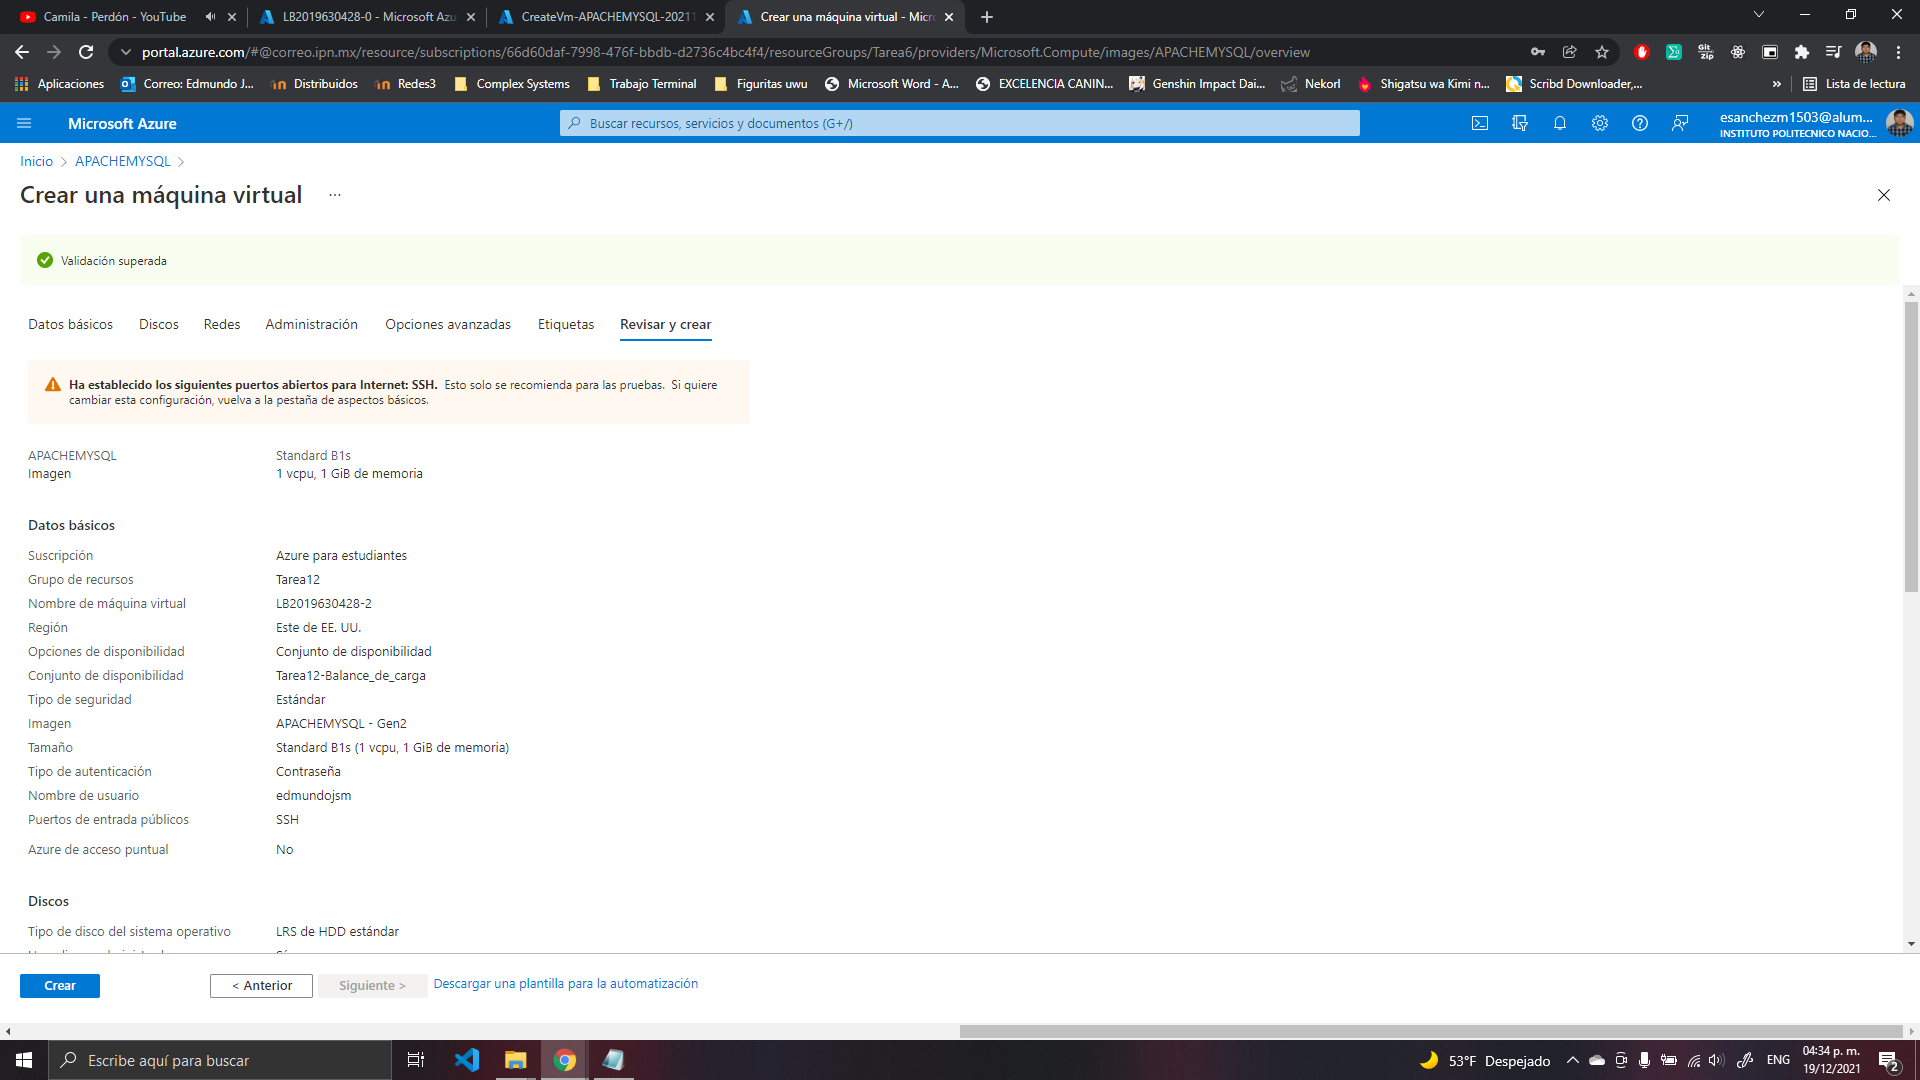
\includegraphics[scale=0.34]{resources/revisarycrear2.png}
			\caption{Creación de la maquina virtual. Nodo 2.}\label{fig:picture}
		\end{figure}
		\begin{figure}[H]
			\centering
			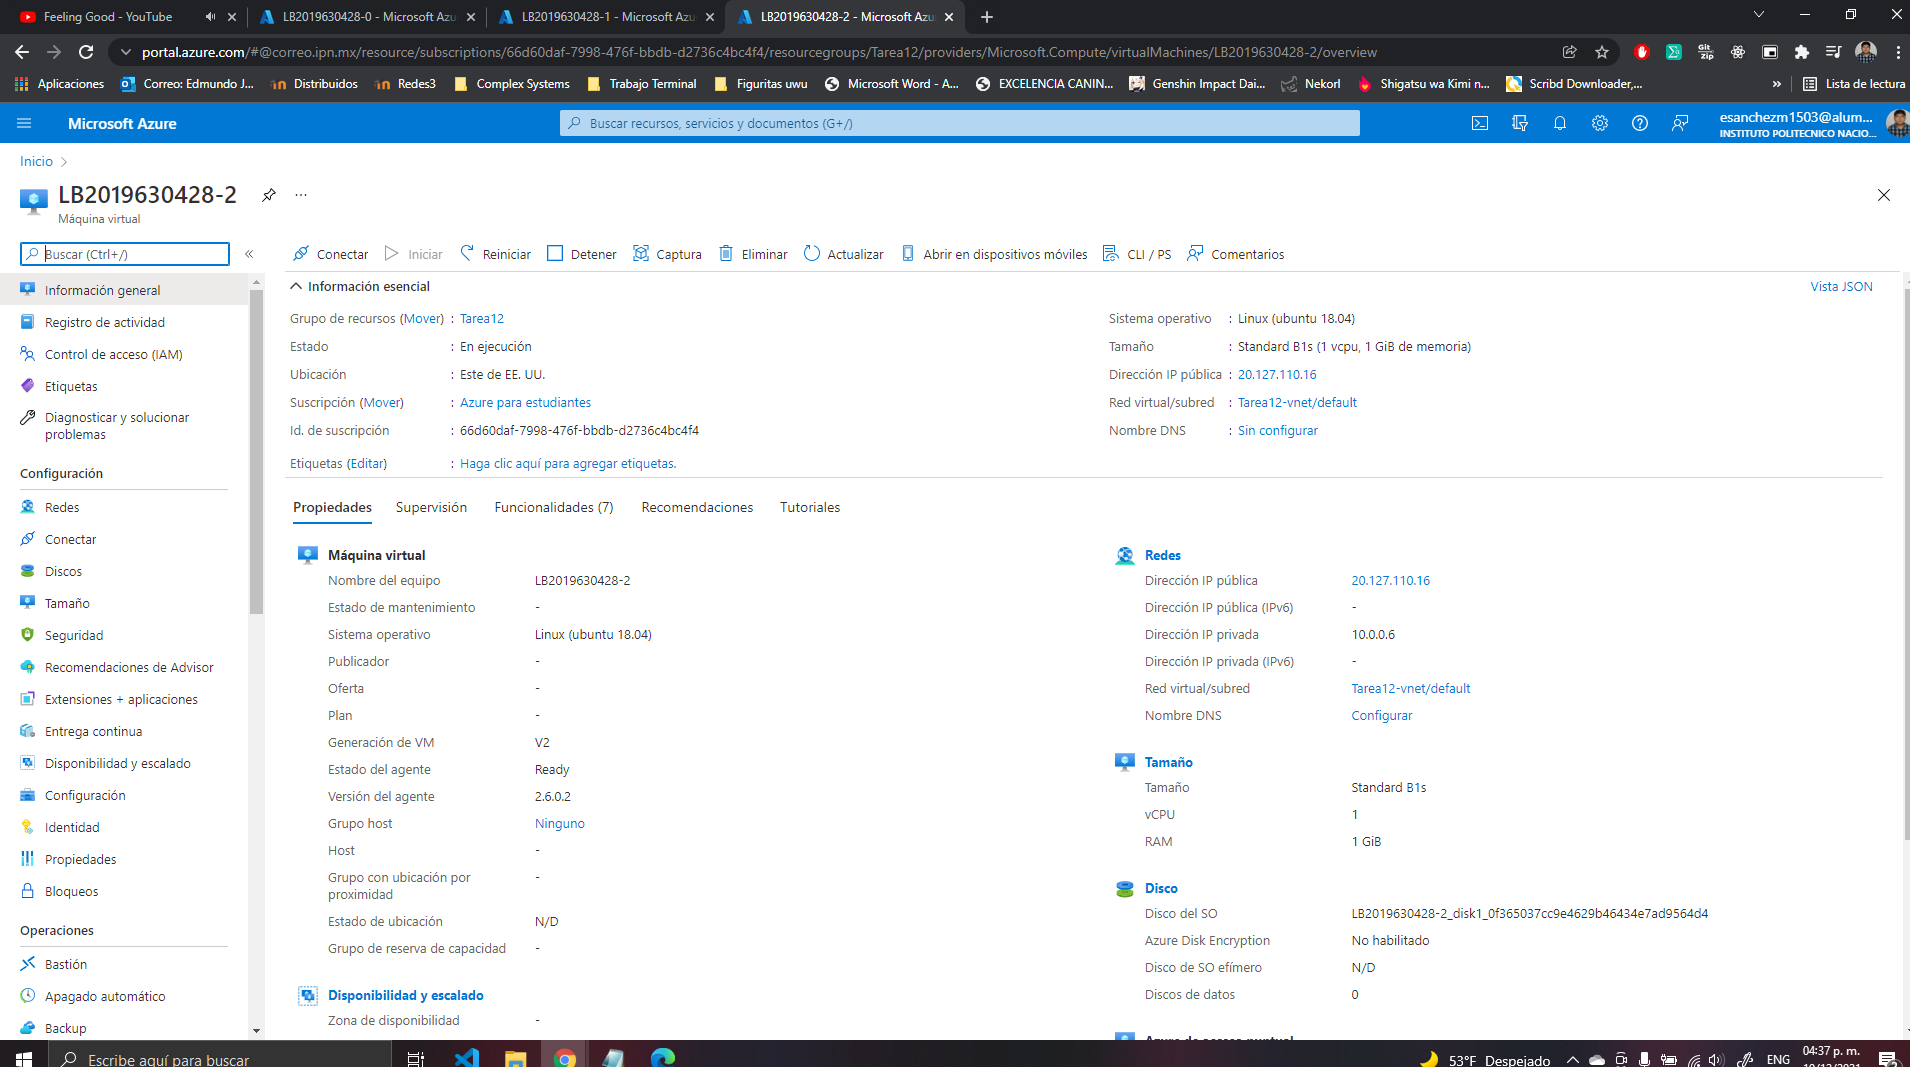
\includegraphics[scale=0.34]{resources/Panelcontrol2.png}
			\caption{Panel de control de la maquina virtual. Nodo 2.}\label{fig:picture}
		\end{figure}
		Finalmente en la figura 20 podemos ver como ya existe el usuario hugo en MYSQL y ademas ya existe la base de datos servicio\_web por lo que ya no es necesario crearlas, ademas de que vemos que ya tenemos registros en ella.
		\begin{figure}[H]
			\centering
			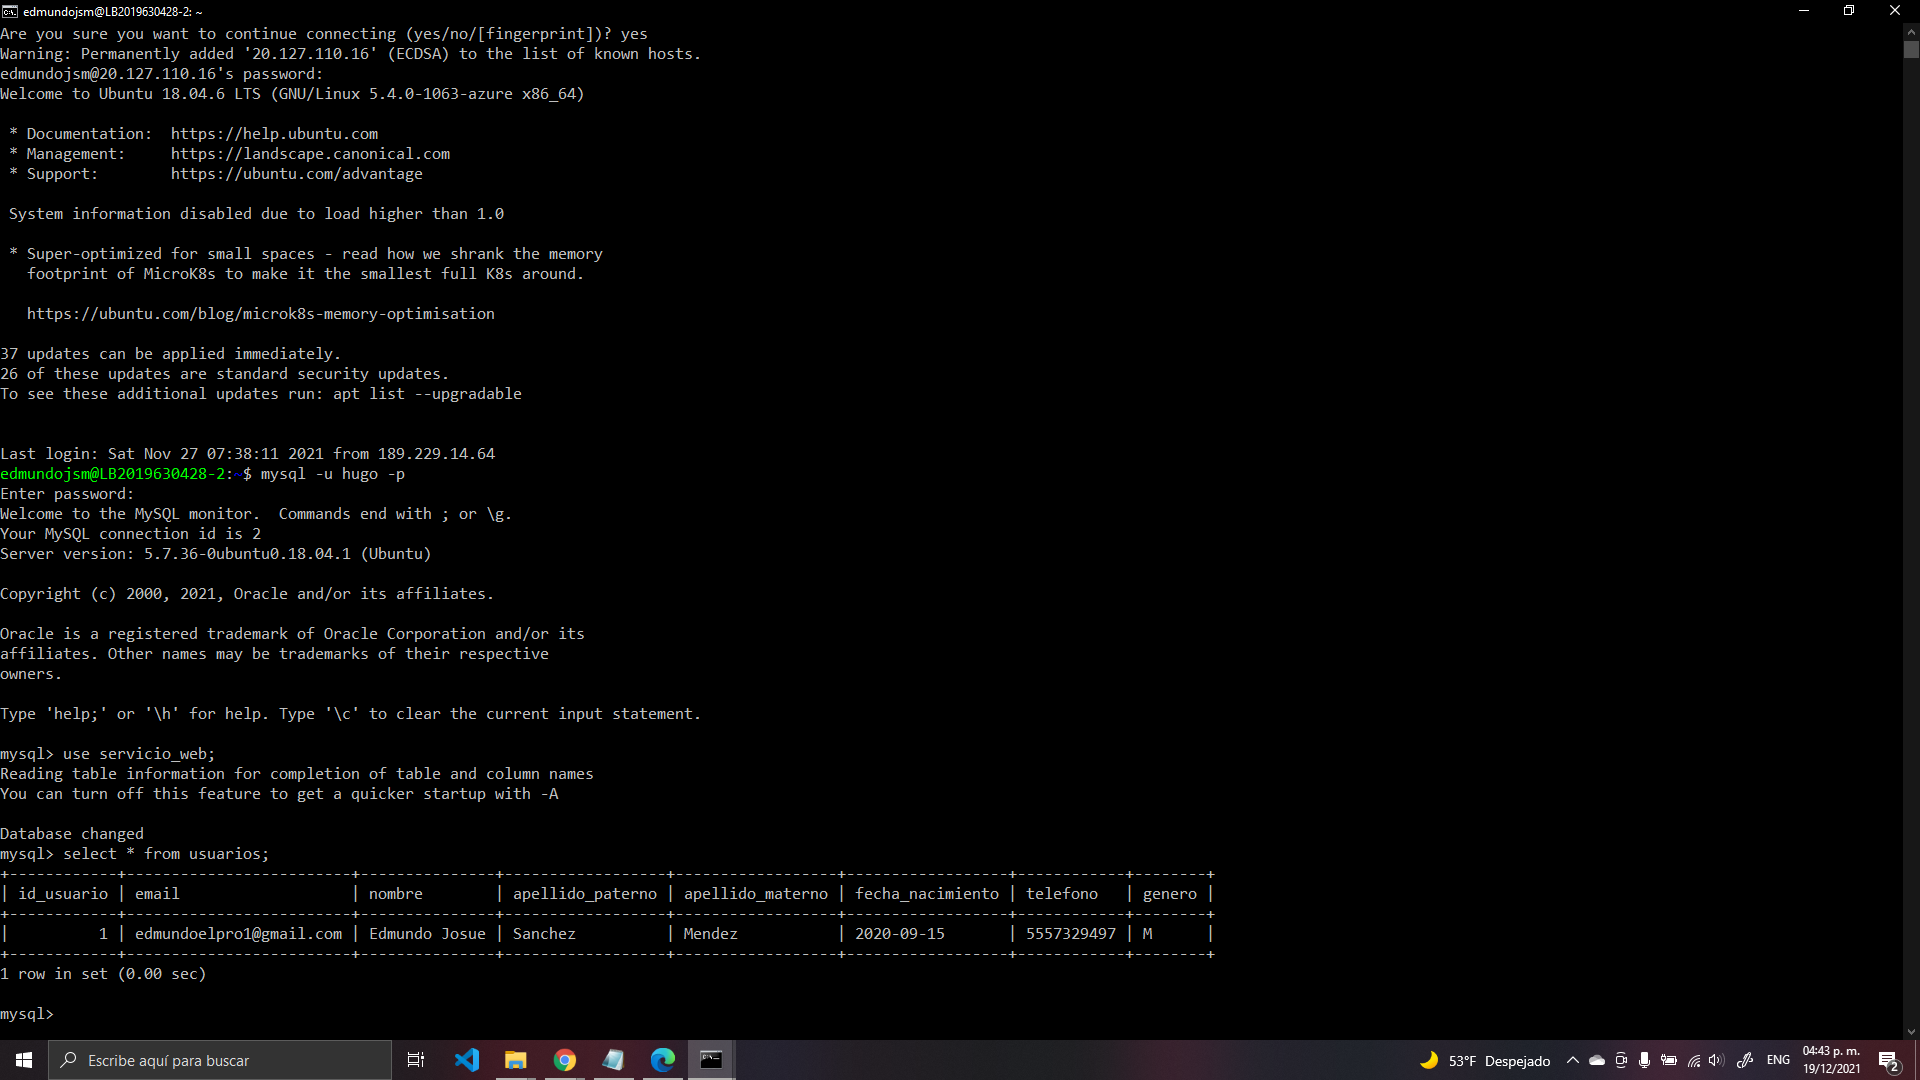
\includegraphics[scale=0.34]{resources/tp3.png}
			\caption{Base de datos y usuarios existentes.}\label{fig:picture}
		\end{figure}
		\subsection{Configuración del servicio web en las dos primeras máquinas virtuales para que cada servicio web se conecte a MySQL que ejecuta en la tercera máquina virtual}
		Para configurar el acceso a MySQL, se modifica el atributo "url" en el archivo "context.xml" del servicio web, en cual se debe cambiar localhost por la IP de la máquina virtual dónde ejecuta MySQL, como vemos en las figuras 21 y 22.
		\begin{figure}[H]
			\centering
			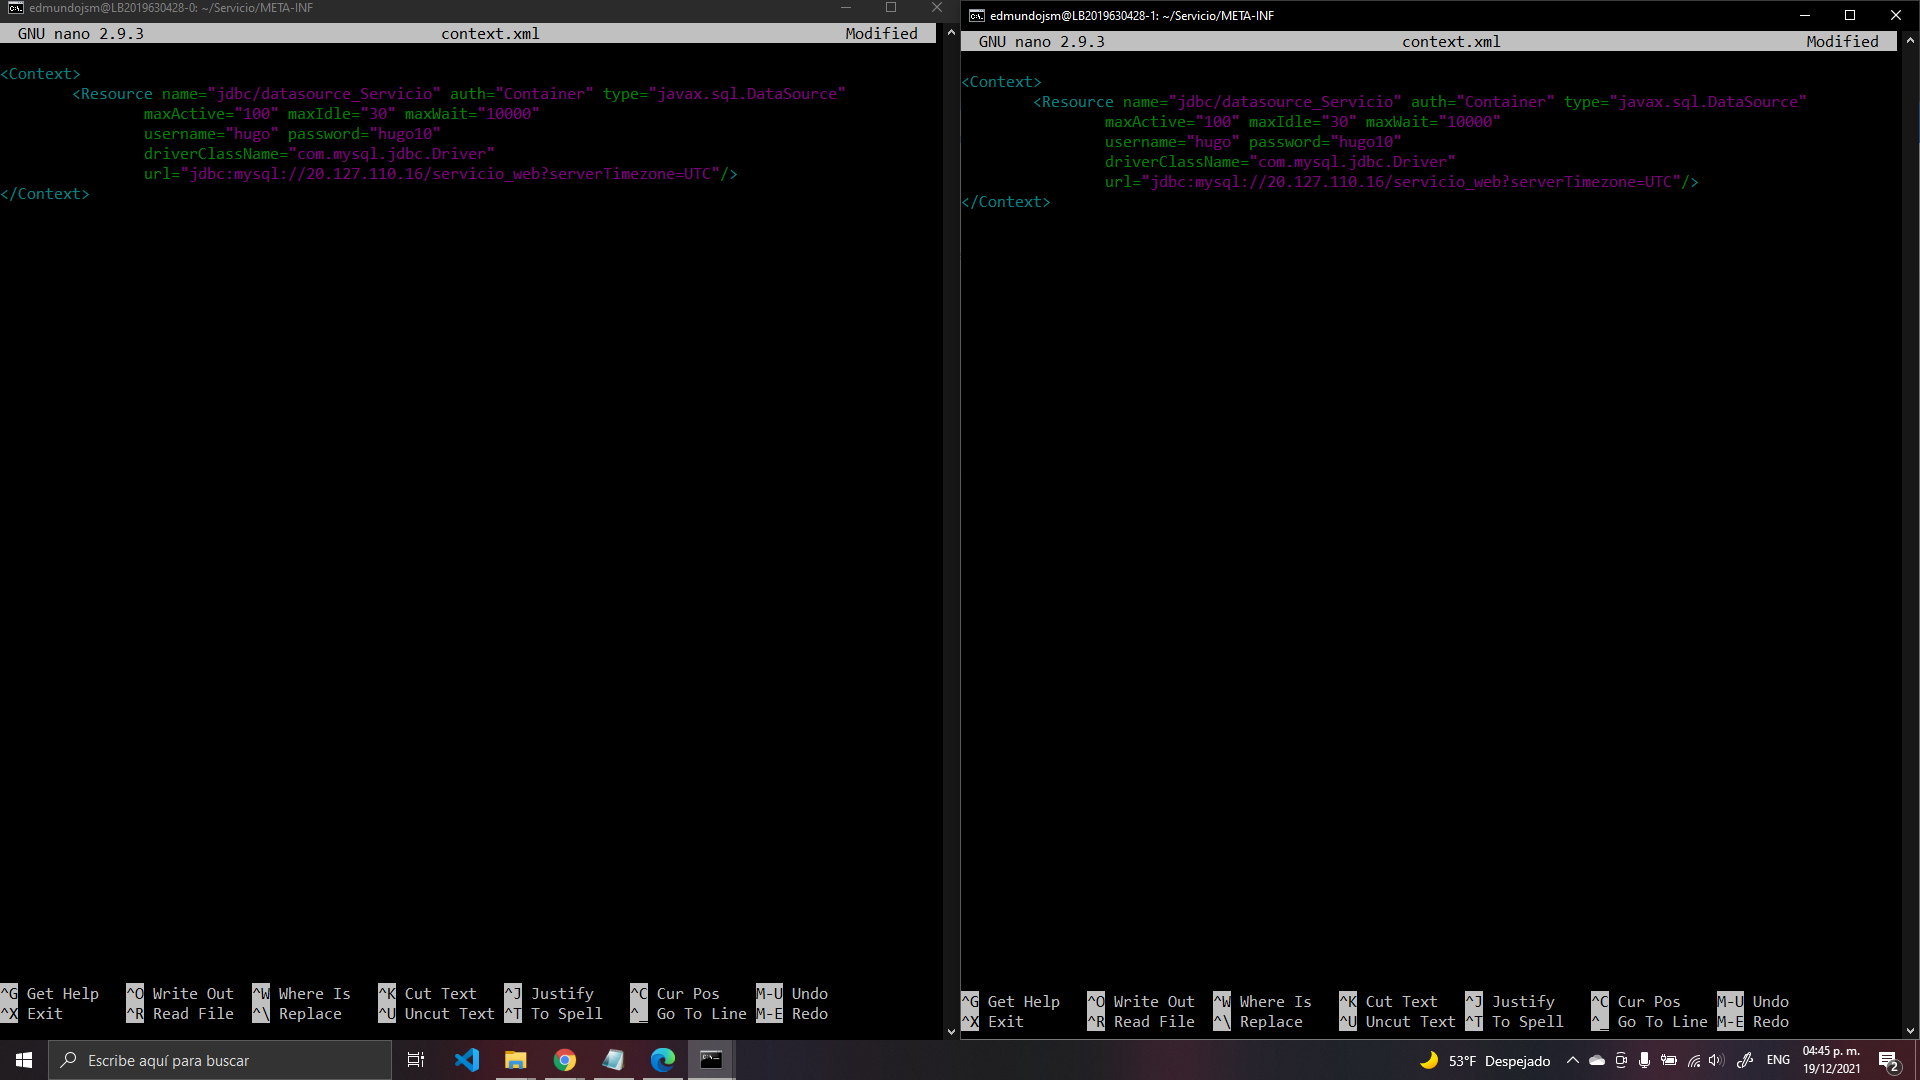
\includegraphics[scale=0.34]{resources/tp4all.png}
			\caption{Cambio del archivo context.xml con la IP de la maquina virtual con MYSQL.}\label{fig:picture}
		\end{figure}
		\begin{figure}[H]
			\centering
			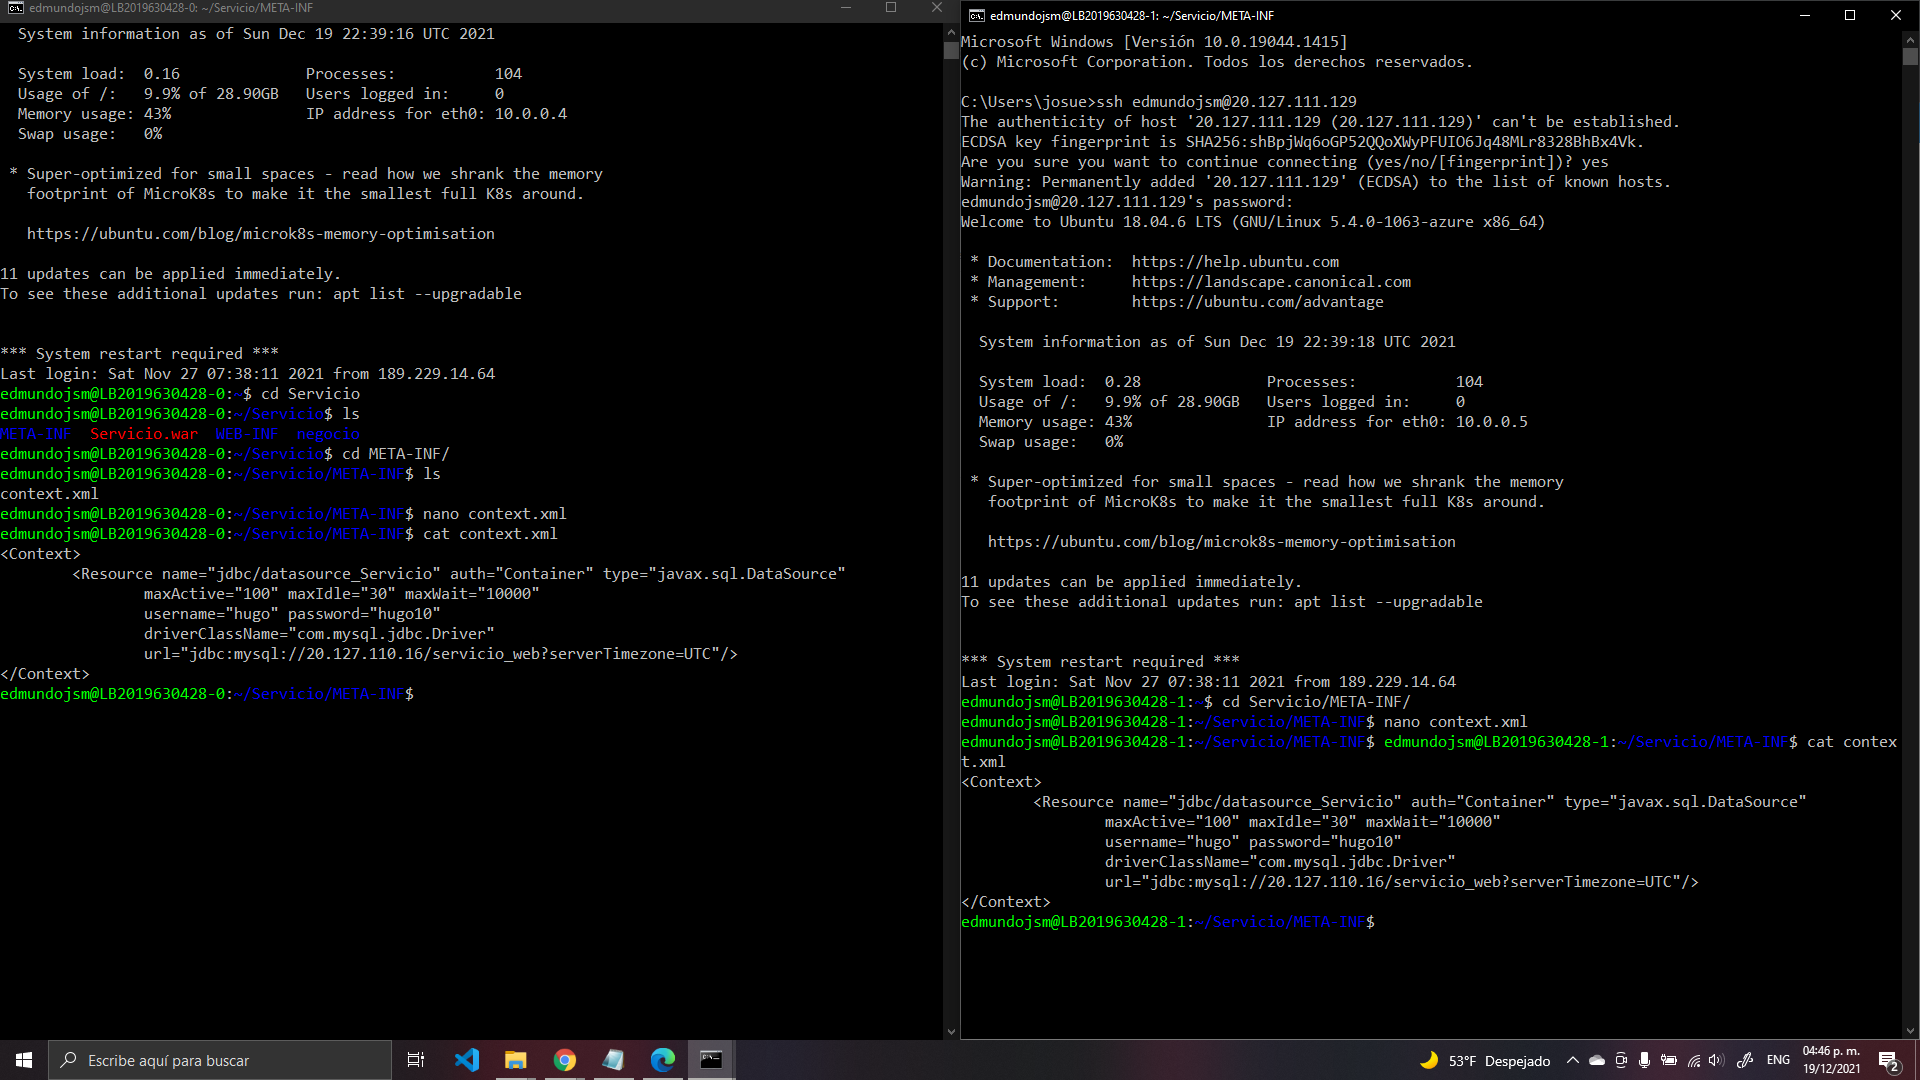
\includegraphics[scale=0.34]{resources/tp4.1.png}
			\caption{Cambio del archivo context.xml realizado.}\label{fig:picture}
		\end{figure}
		Finalmente se creara el servicio web para Tomcat con el cambio realizado en ambas maquinas virtuales, ademas de copiar el .war a webapps de Tomcat, sin embargo, esto no es suficiente ya que necesitamos habilitar conexión remota a MYSQL. Primero tenemos que permitir a MySQL escuchar tráfico externo, para ello es necesario que se habilite la escucha de direcciones IP externas, para activar esto, se tiene que modificar el archivo mysqld.cnf, ahí se tendrá que modificar una linea que empieza con la directiva bind-address, por defecto el valor asignado es 127.0.0.1 y se tendrá que modificar por una IP externa que se conectara con MYSQL o con comodines para para permitir conexiones remotas en general, sin restringir a direcciones IP específicas, para esto asignamos el valor como *, ::, o 0.0.0.0. Se guarda el documento y reiniciamos el demonio de MYSQL para que los cambios realizados tengan efecto, esto lo podemos ver en las figuras 23 y 24.
		\begin{figure}[H]
			\centering
			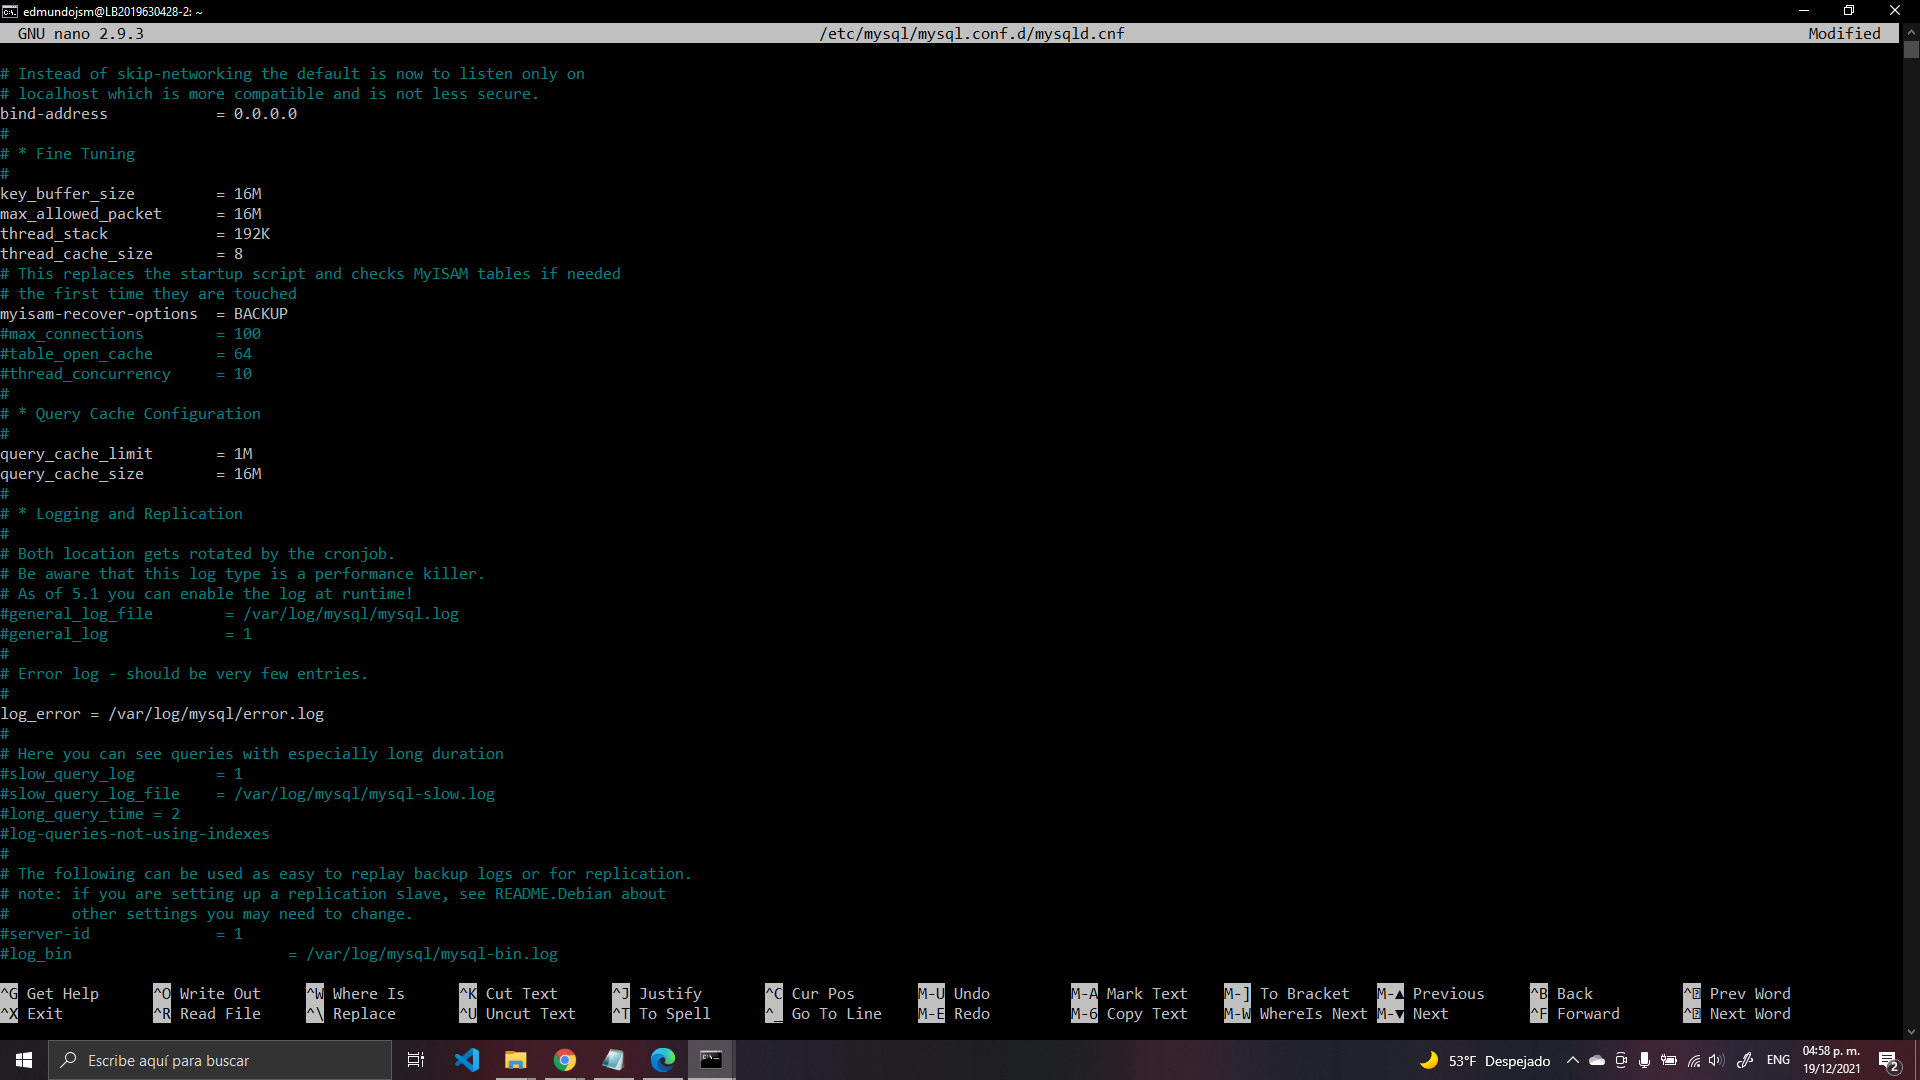
\includegraphics[scale=0.34]{resources/conexionesremotasMYSQL.png}
			\caption{Permitir a MySQL escuchar tráfico externo.}\label{fig:picture}
		\end{figure}
		\begin{figure}[H]
			\centering
			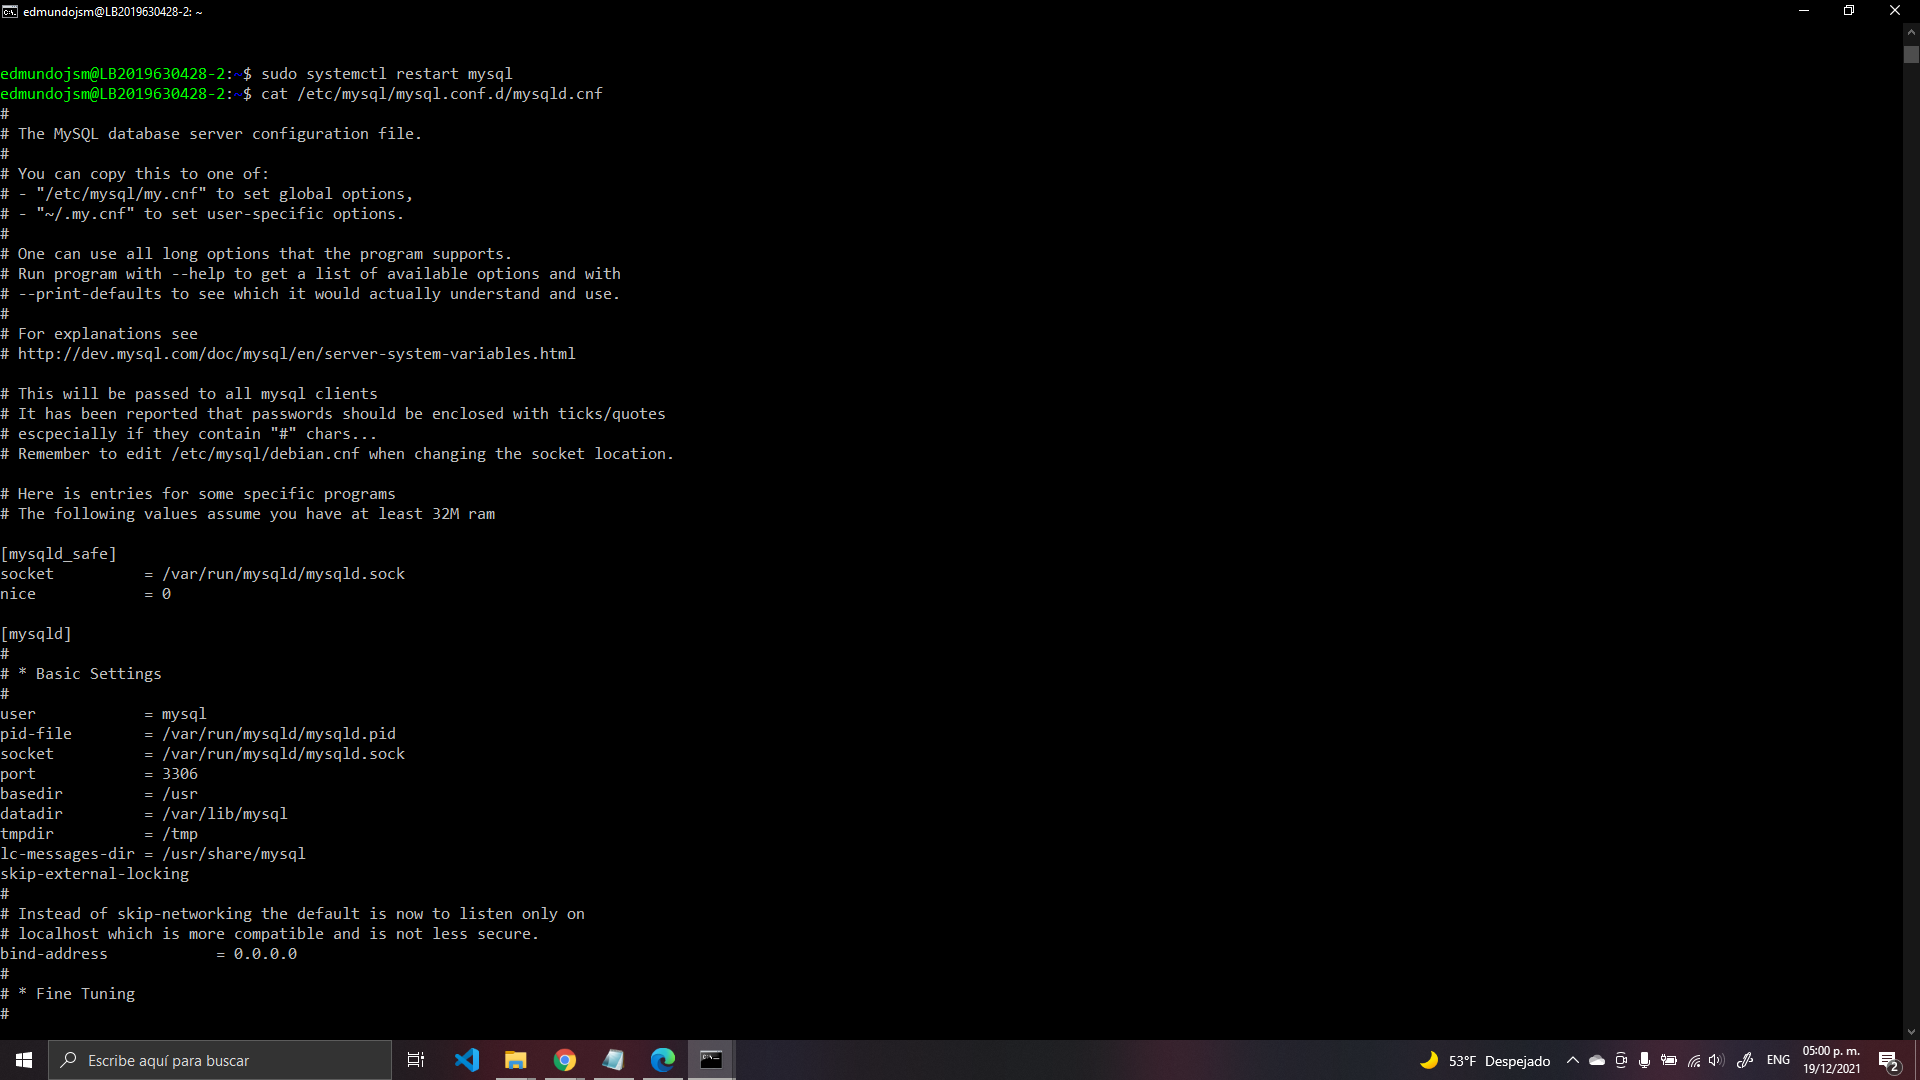
\includegraphics[scale=0.34]{resources/conexionesremotasMYSQ1.png}
			\caption{Demonio reiniciado con los cambios realizados con éxito.}\label{fig:picture}
		\end{figure}
		Ahora actualizamos el usuario hug, para cambiar el host de un usuario, podemos usar el comando RENAME USER de MySQL. Como vemos en la figura 25, mencionar que al final del comando se ingresa el carácter \% para permitir que cualquier IP pueda usar el usuario hugo.
		\begin{figure}[H]
			\centering
			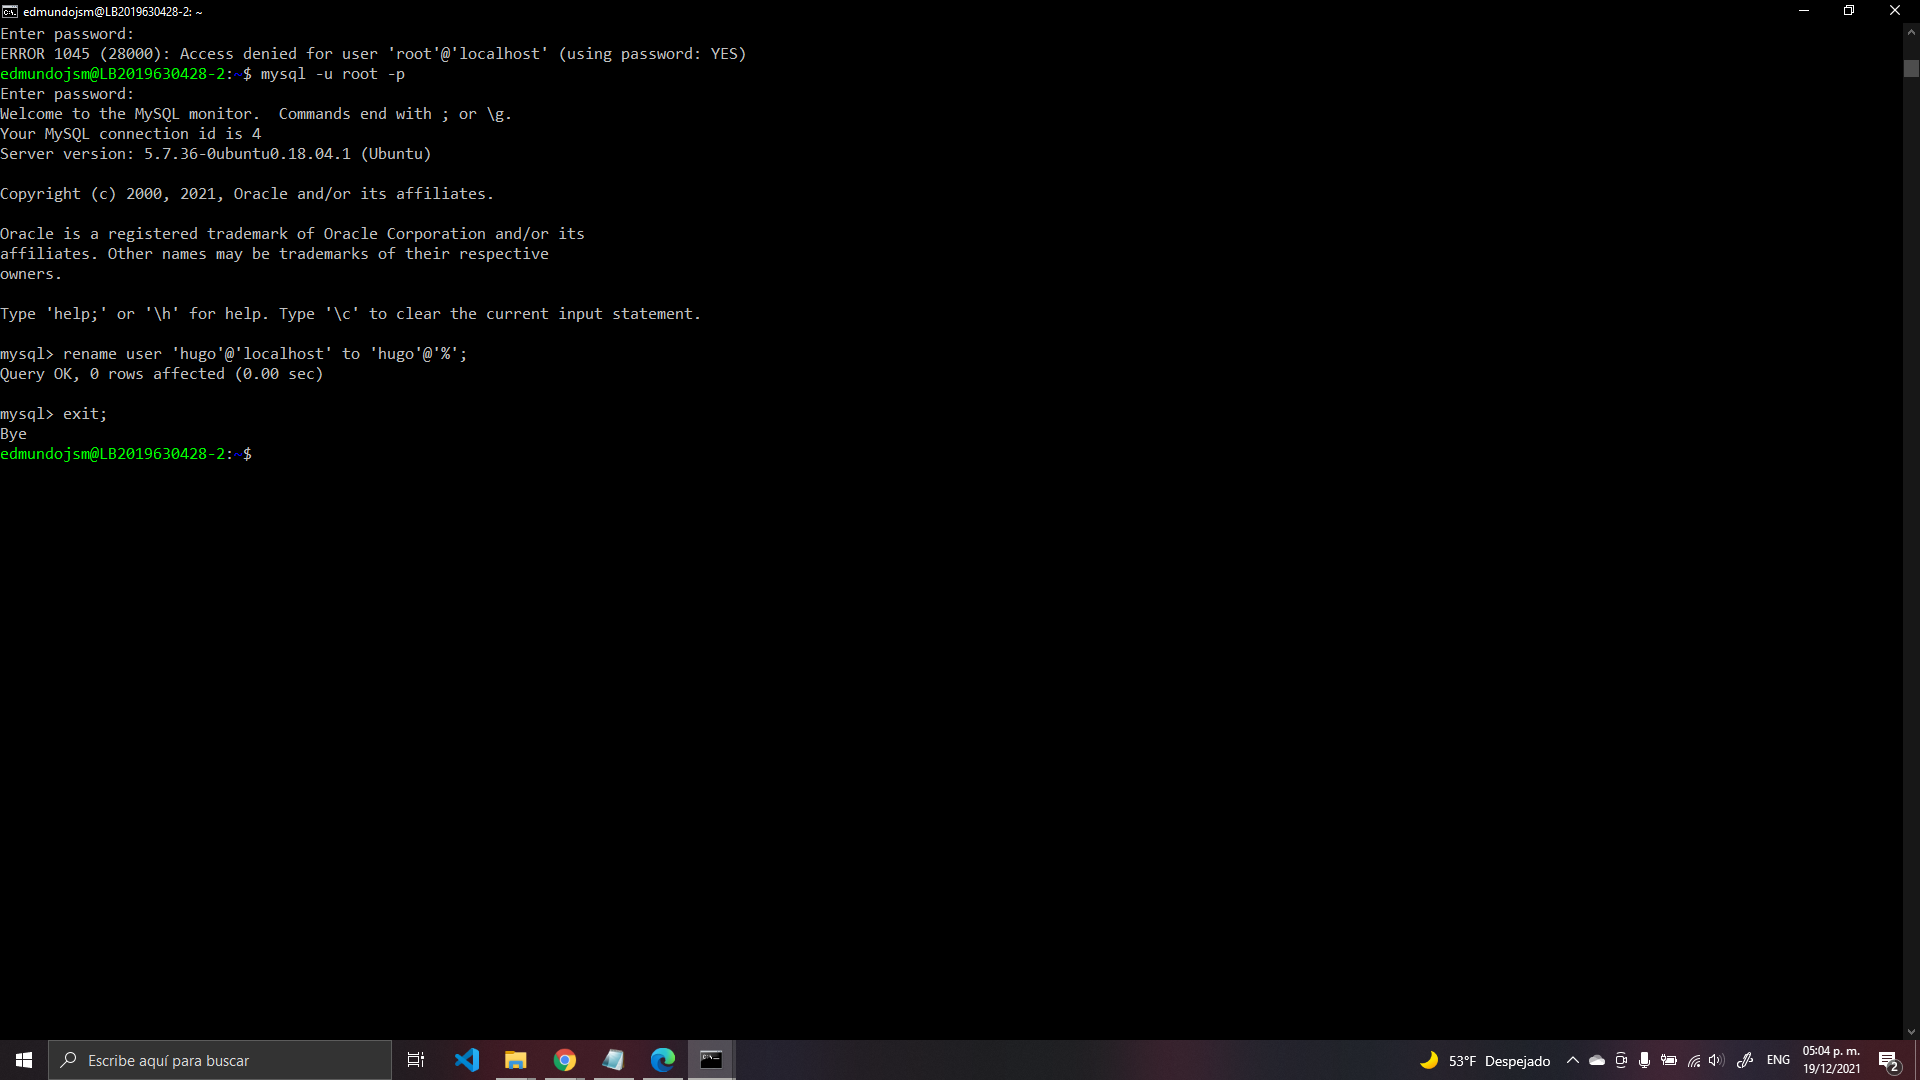
\includegraphics[scale=0.34]{resources/conexionesremotasMYSQ3.png}
			\caption{Actualización del usuario hugo.}\label{fig:picture}
		\end{figure}
		
		\subsection{Utilizar la aplicación web prueba.html para probar que el servicio web en cada máquina virtual tenga acceso a la base de datos en MySQL.}	
		Antes de probarlo, nos damos cuenta que tenemos que hacer modificaciones a los puertos de las maquinas virtuales ya que tenemos que abrir el puerto 8080 de cada una para tener acceso al servicio web, como vemos en las figuras 26 y 27, estos dos pasos nos servira mas adelante para la implementacion del balance de carga.
		\begin{figure}[H]
			\centering
			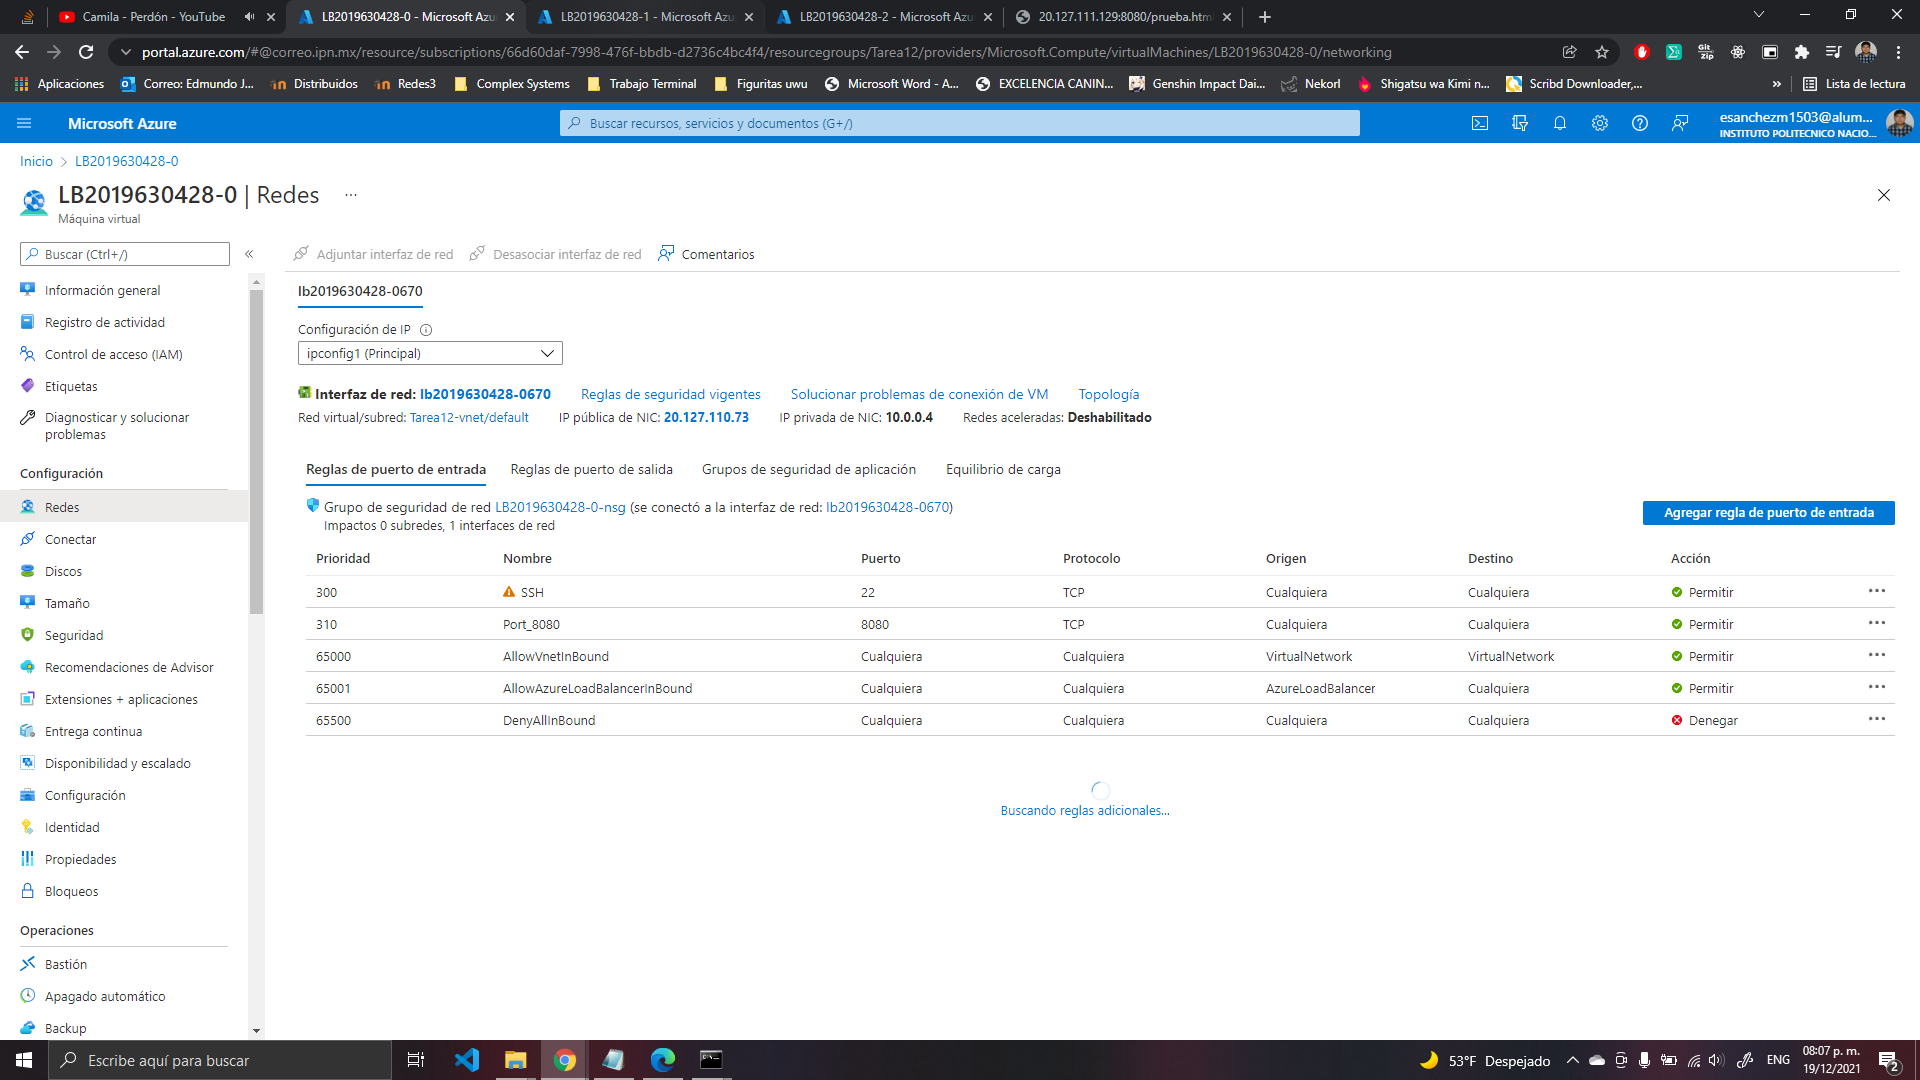
\includegraphics[scale=0.34]{resources/8080N0.png}
			\caption{Puerto 8080 abierto en el nodo 0.}\label{fig:picture}
		\end{figure}
		\begin{figure}[H]
			\centering
			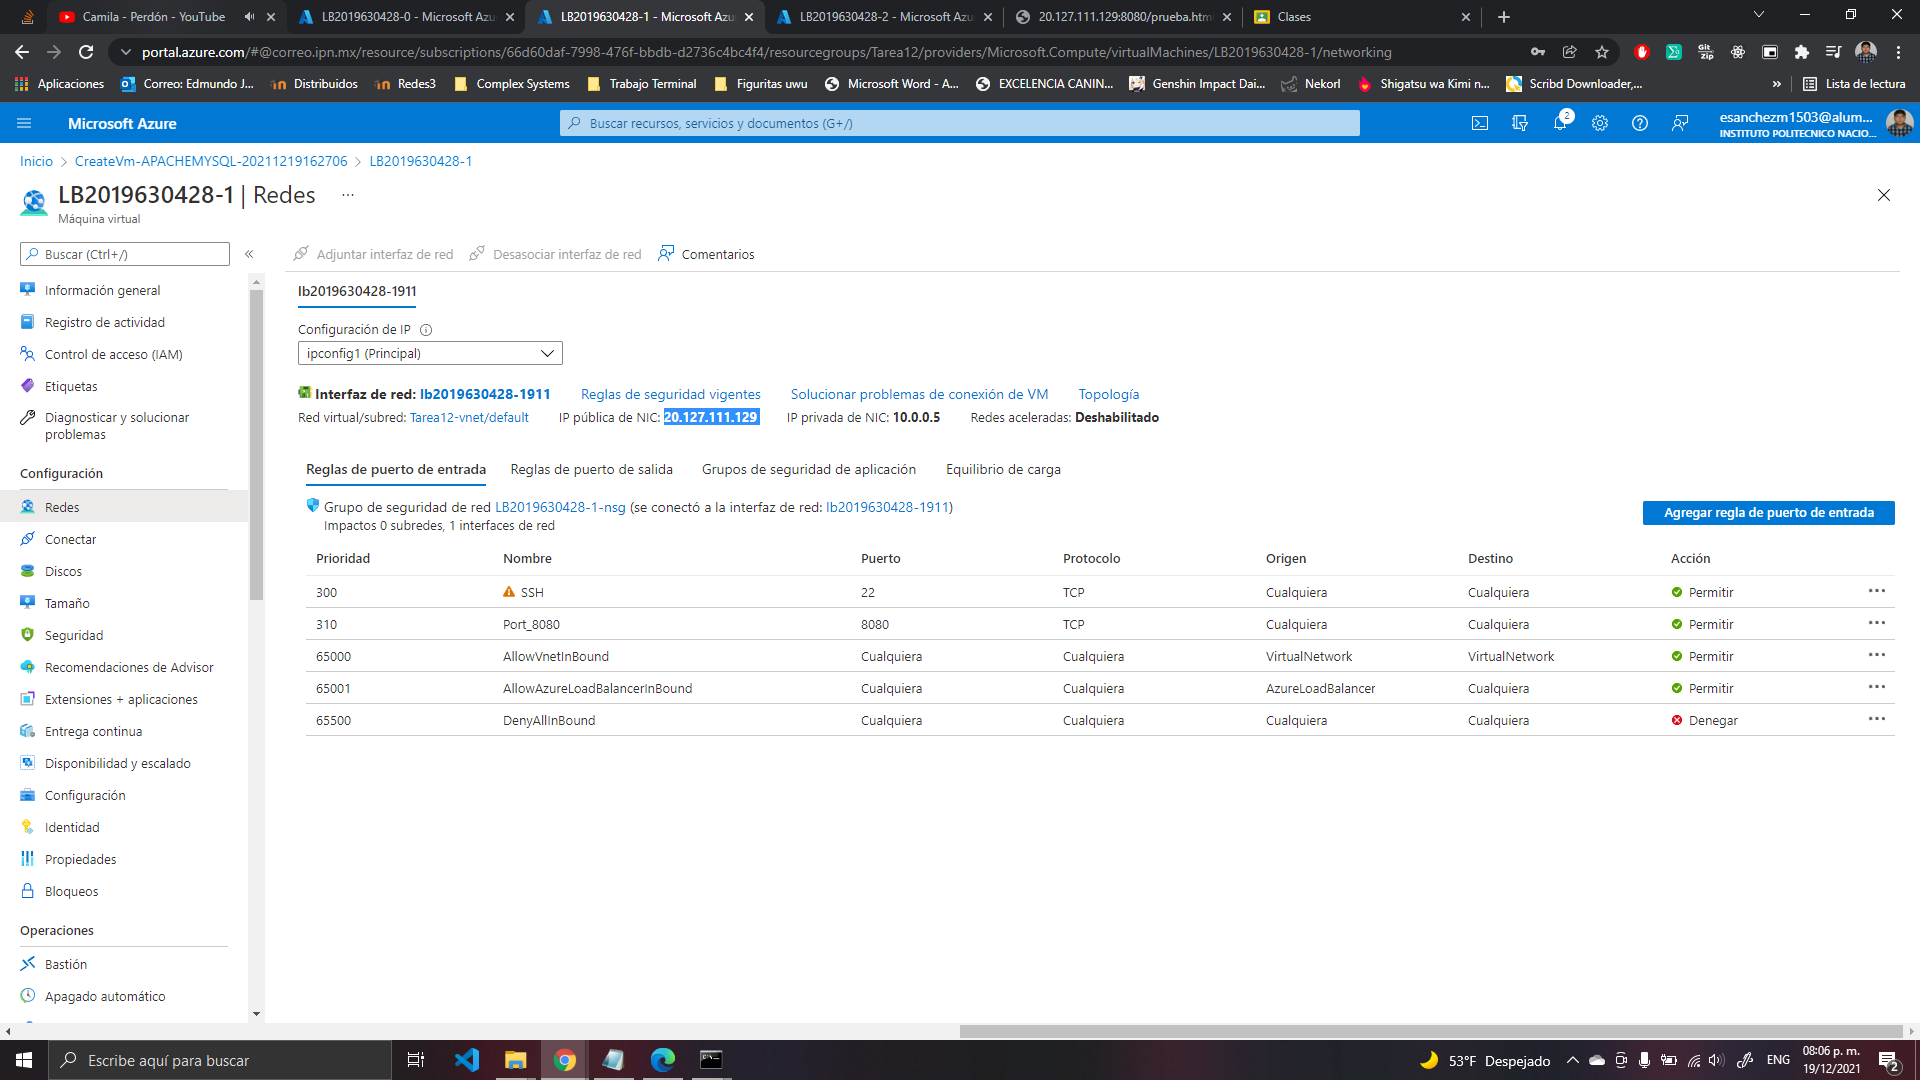
\includegraphics[scale=0.34]{resources/8080N1.png}
			\caption{Puerto 8080 abierto en el nodo 1.}\label{fig:picture}
		\end{figure}
		Sin embargo, nos encontramos con otro problema como vemos en la figura 28 para ello tenemos que comentar o eliminar la linea request.setRequestHeader(``Content-length'', body.length); como vemos en la figura 29, este problema es provocado ya que XMLHttpRequest no puede configurar estos encabezados, el navegador los configura automáticamente. La razón es que al manipular estos encabezados, es posible que se pueda engañar al servidor para que acepte una segunda solicitud a través de la misma conexión, una que no pasaría por las comprobaciones de seguridad habituales; eso sería una vulnerabilidad de seguridad en el navegador.
		\begin{figure}[H]
			\centering
			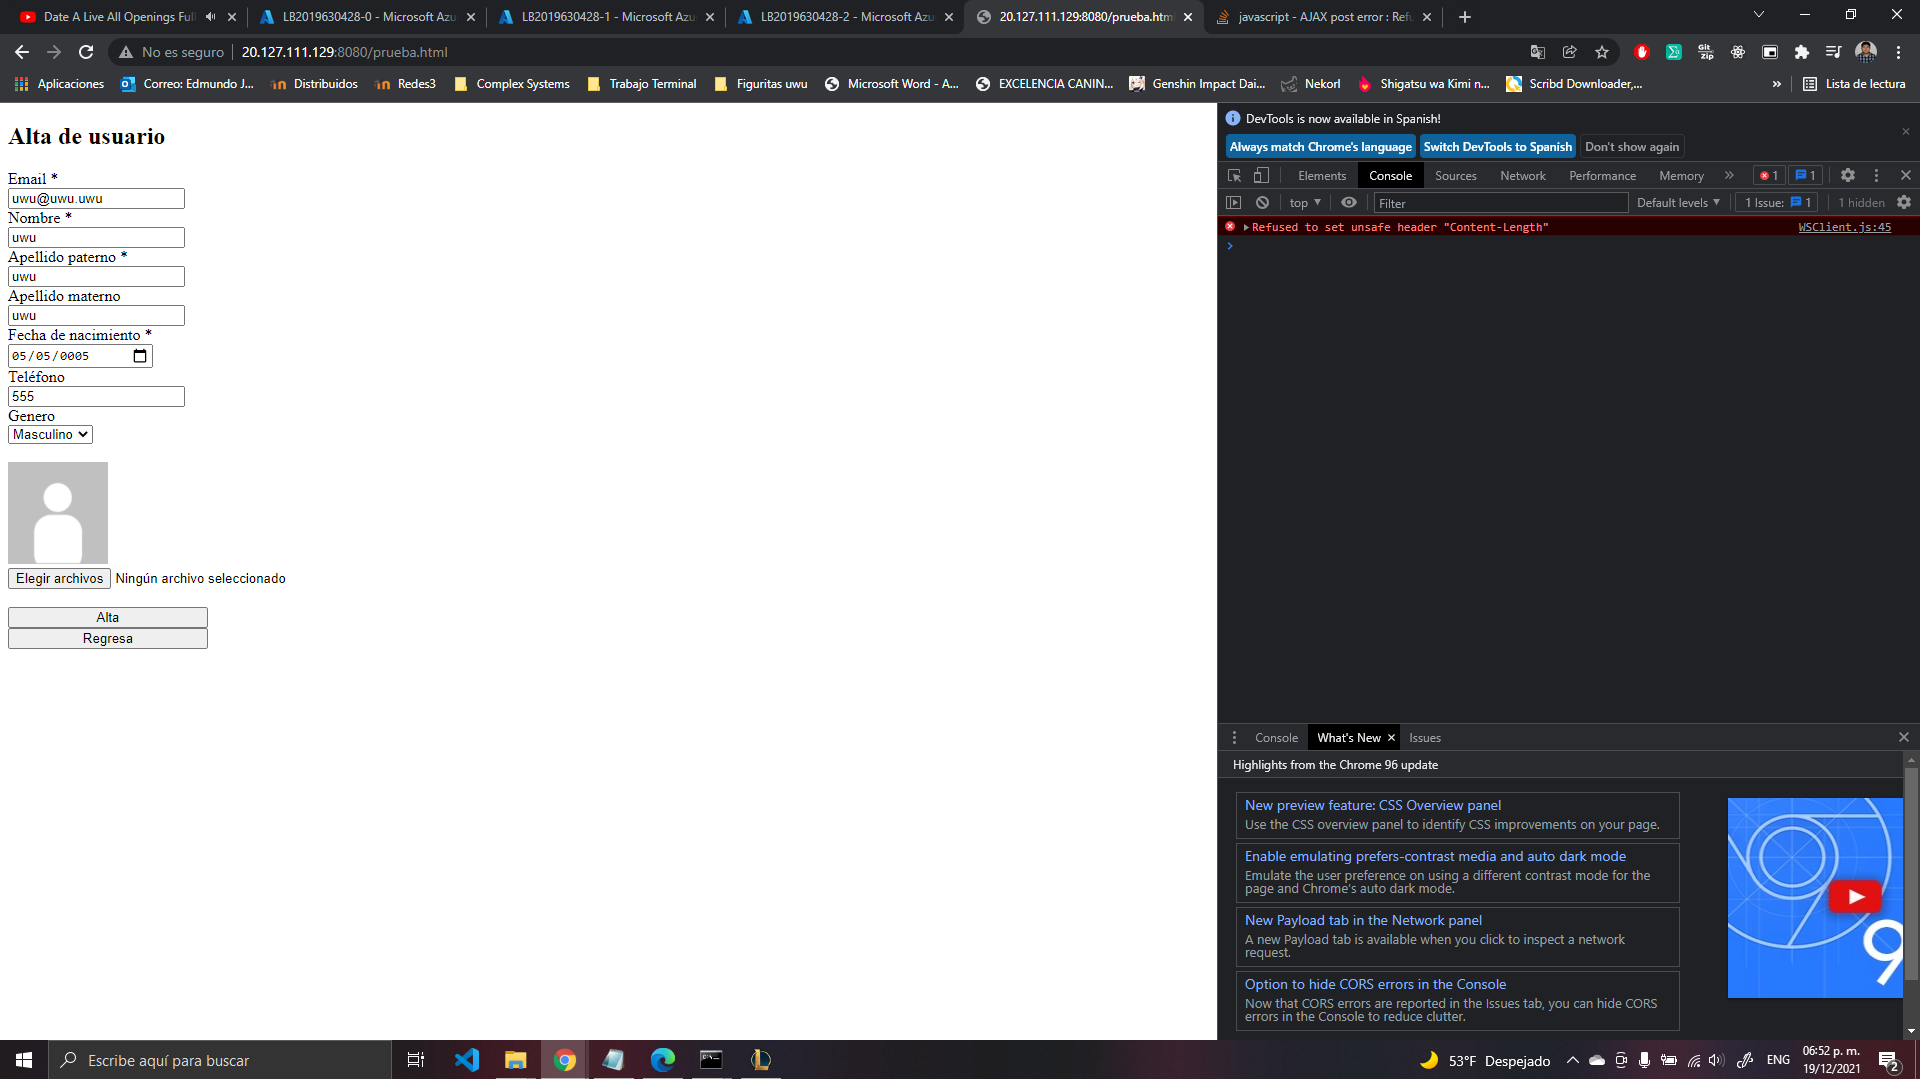
\includegraphics[scale=0.34]{resources/problema1.png}
			\caption{Problema con JavaScript.}\label{fig:picture}
		\end{figure}
		\begin{figure}[H]
			\centering
			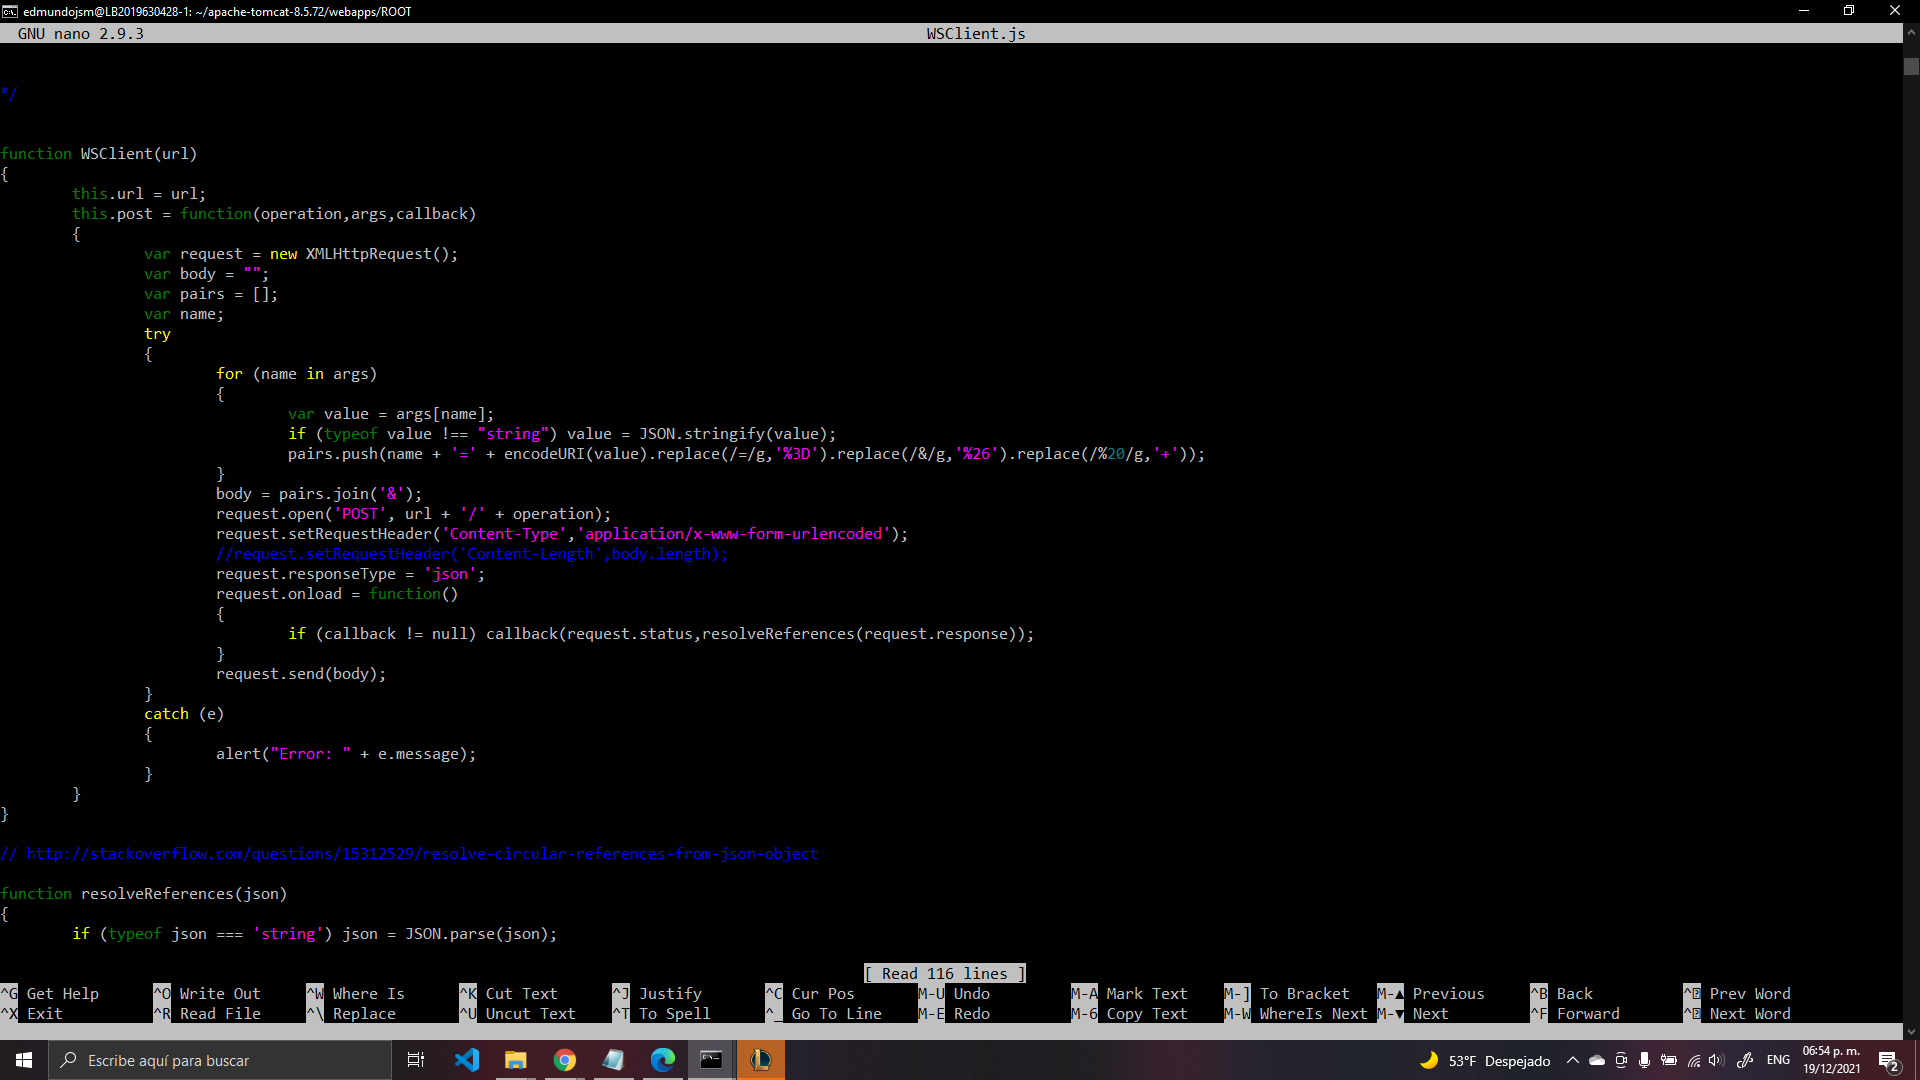
\includegraphics[scale=0.34]{resources/solucionproblema1.png}
			\caption{Solución del problema con JavaScript.}\label{fig:picture}
		\end{figure}
		Finalmente veamos las pruebas en la figura 30 en ambas maquinas virtuales, del lado izquierdo tenemos al nodo 0 y del lado derecho tenemos al nodo 1. Podemos ver en la figura 31 como en la base de datos que tenemos en el nodo 2 el registro de usuario fue realizado de manera correcta.
		\begin{figure}[H]
			\centering
			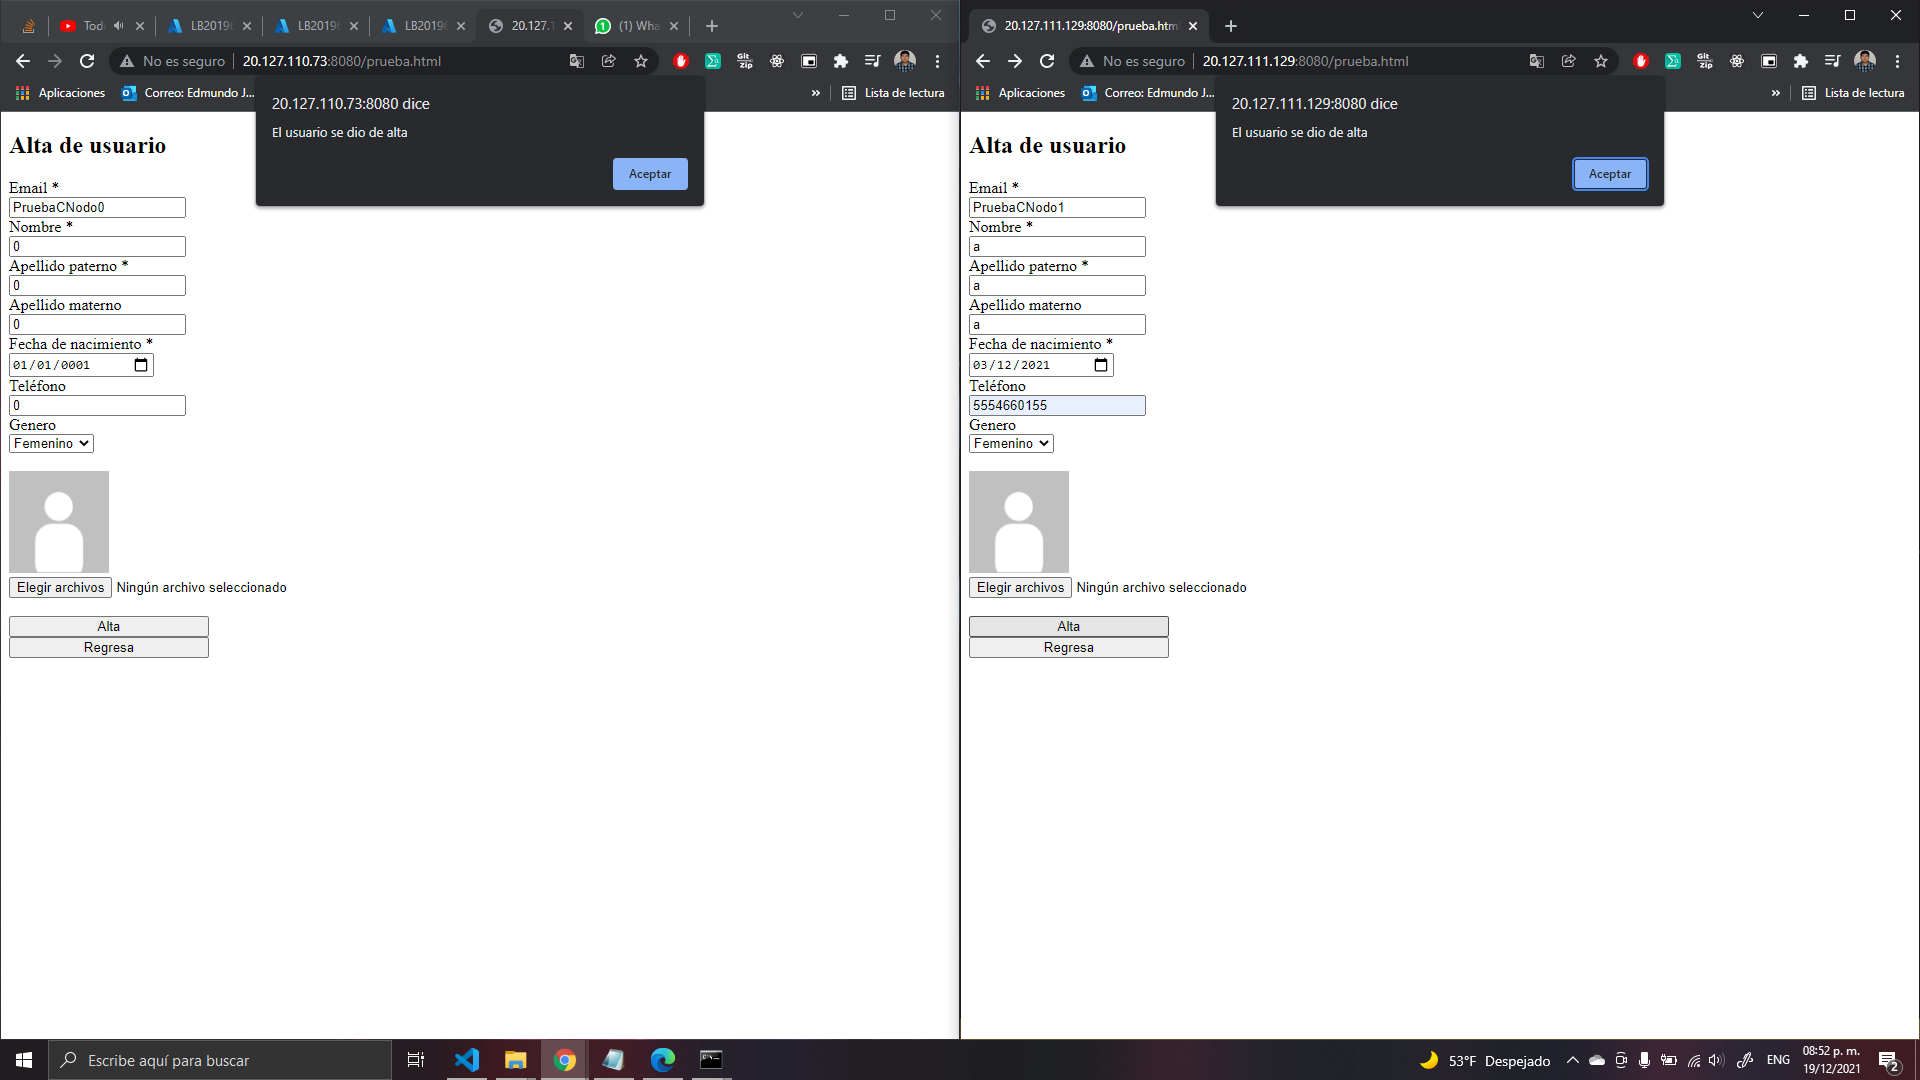
\includegraphics[scale=0.34]{resources/tp5.1.png}
			\caption{Pruebas del servicio.}\label{fig:picture}
		\end{figure}
		\begin{figure}[H]
			\centering
			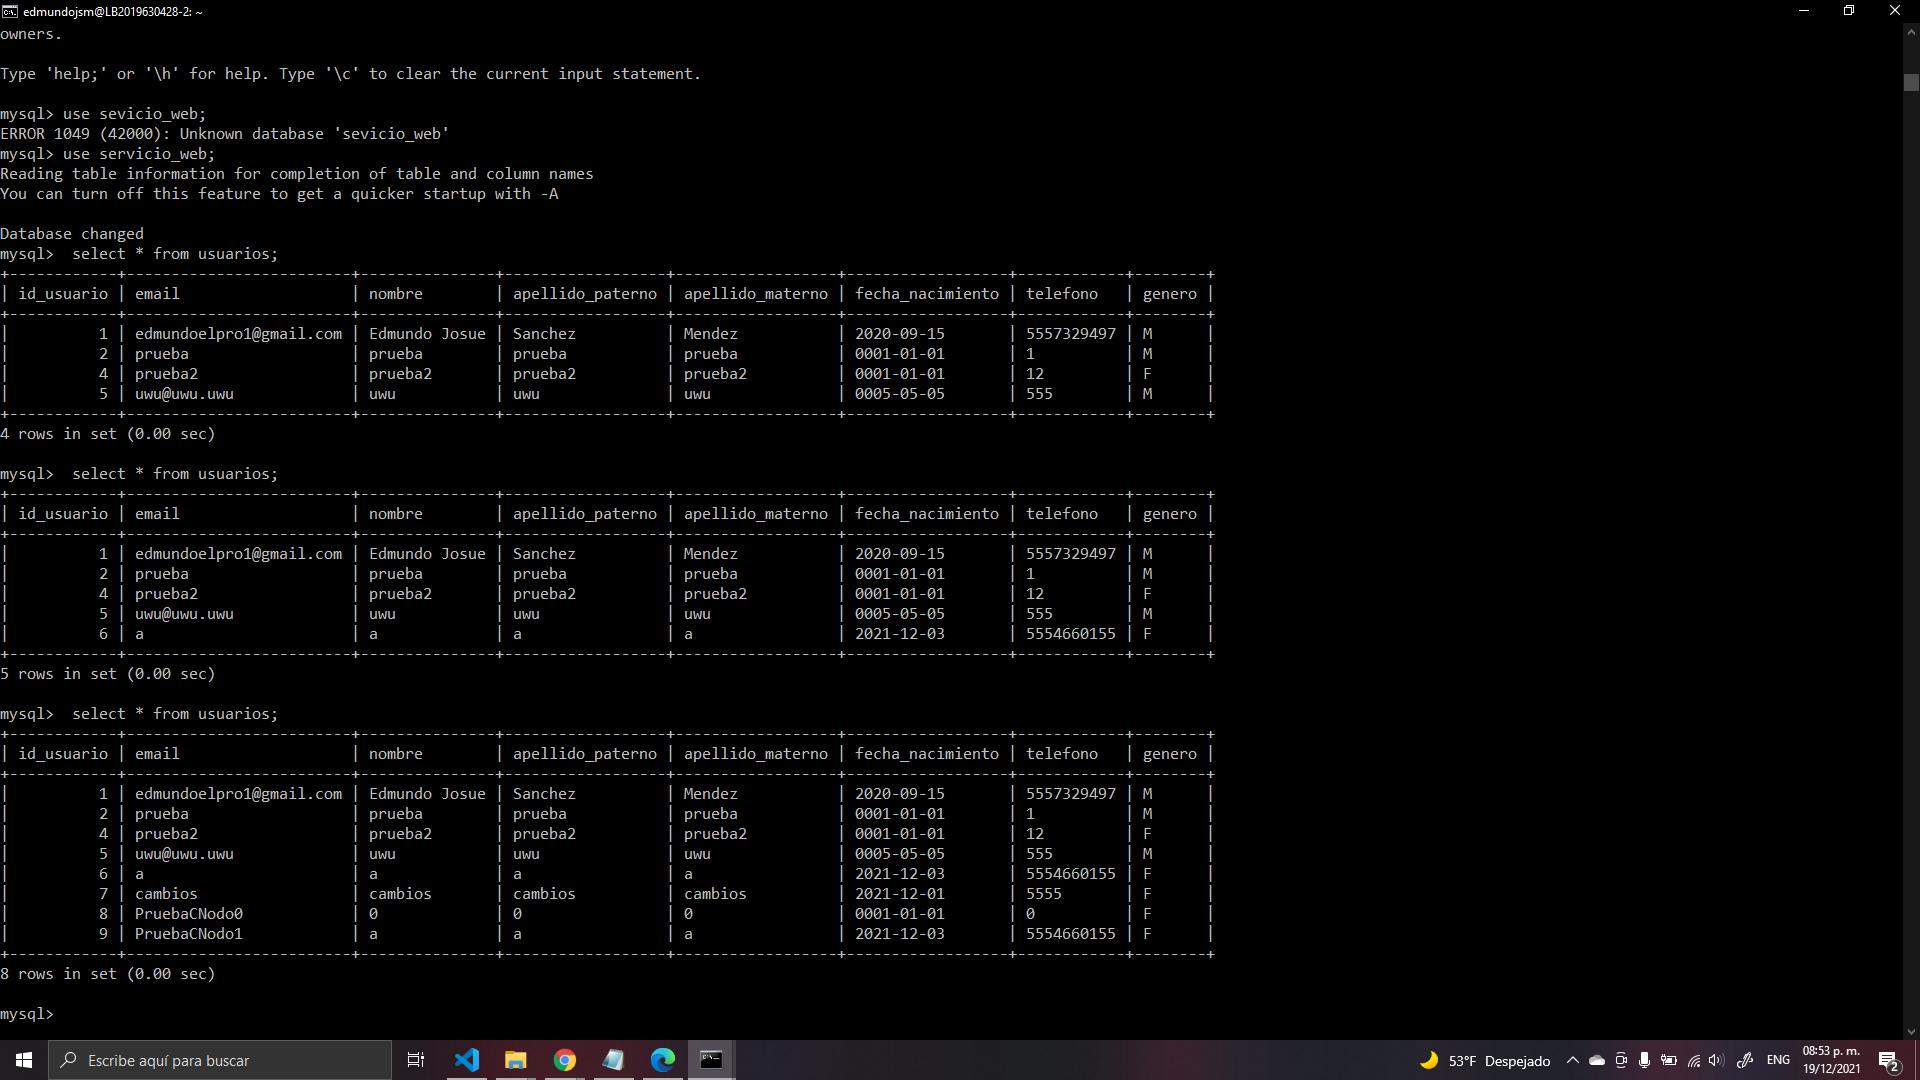
\includegraphics[scale=0.34]{resources/tp5.2.png}
			\caption{Base de datos después de la prueba.}\label{fig:picture}
		\end{figure}
		\subsection{Quitar la IP pública a las máquinas virtuales dónde ejecuta Tomcat}
		Una vez que ya verificamos que funciona el servicio debemos de quitar la IP publica de las maquinas virtuales, mencionar que esto se puede hacer desde la creación de la maquina virtual, sin embargo, no podríamos hacer la prueba anterior. Para ello seleccionar la máquina virtual, seleccionar la IP pública, seleccionar la opción ``Información general'', y seleccionar la opción ``Desasociar''. Esto lo podemos ver en las figuras 32 y 33.	
		\begin{figure}[H]
			\centering
			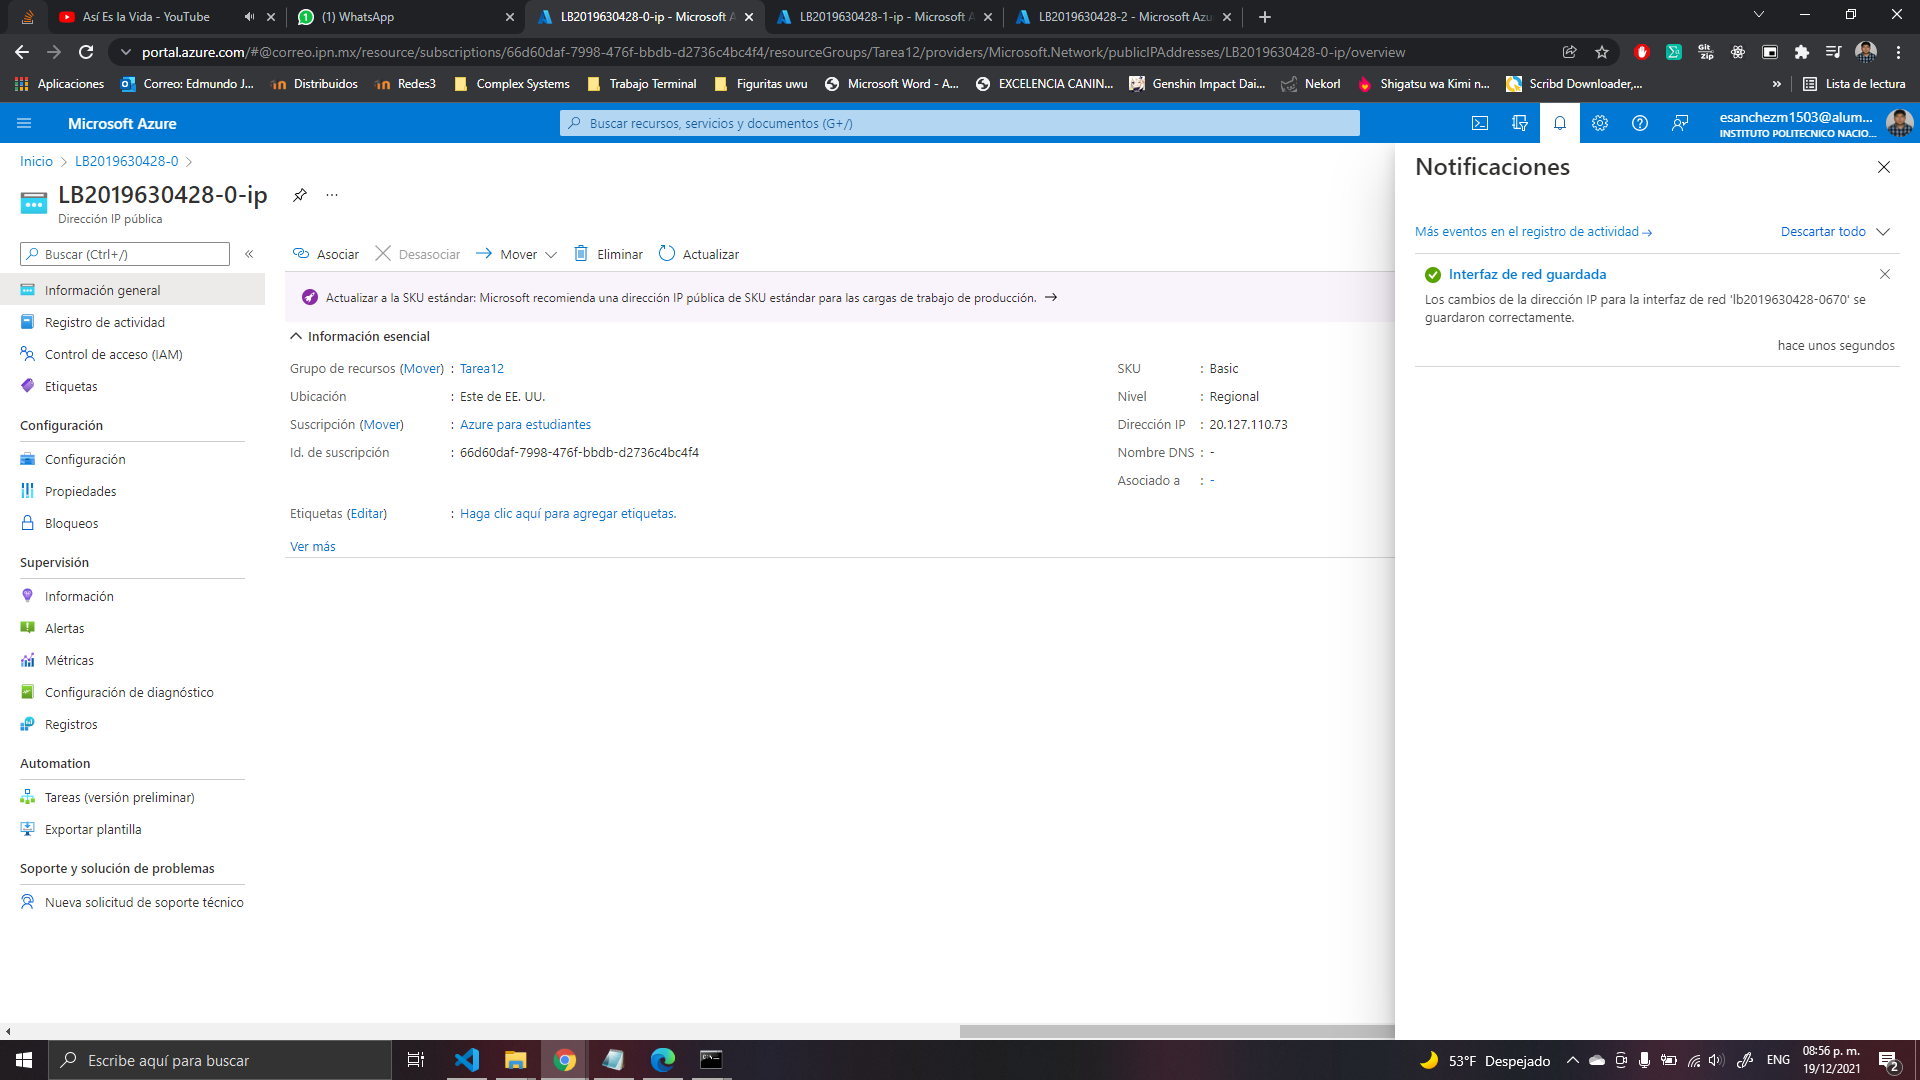
\includegraphics[scale=0.34]{resources/tp6N0.png}
			\caption{IP publica quitada en el nodo 0.}\label{fig:picture}
		\end{figure}
		\begin{figure}[H]
			\centering
			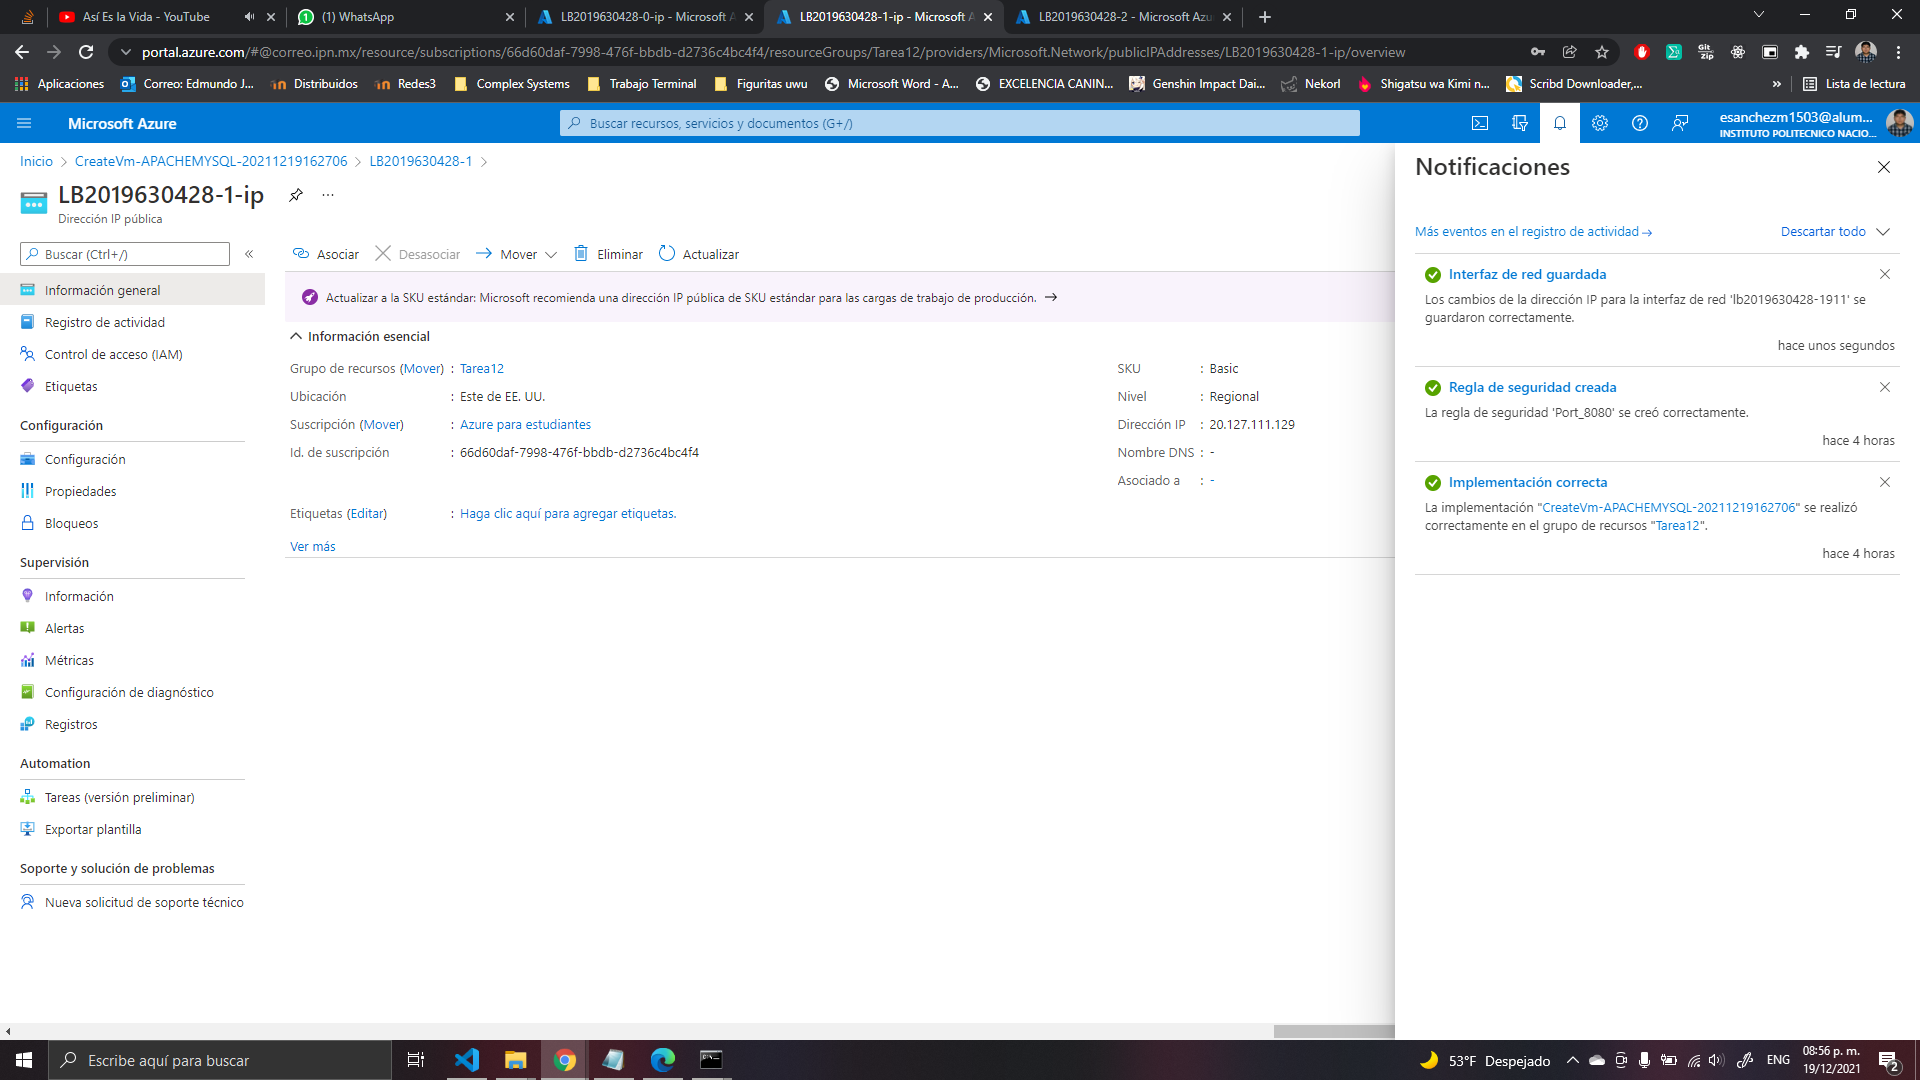
\includegraphics[scale=0.34]{resources/tp6N1.png}
			\caption{IP publica quitada en el nodo 1.}\label{fig:picture}
		\end{figure}
		\subsection{Creación de un balanceador de carga y conexión a las máquinas virtuales creadas en el paso 1}
		Ahora veamos la creación del balanceador de carga, veamos paso a paso.
			\subsubsection{Creación de un balanceador de carga en Azure}
			Para esto tenemos que ir Equilibradores de carga como vemos en la figura 34, después nos vamos a la opción de ``+Crear'' y ahora seleccionamos el grupo de recursos o bien, creamos un nuevo grupo de recursos, sin embargo, como ya tenemos nuestro grupo de recursos ya no es necesario, despues ingresamos un nombre para la instancia del balanceador de carga, seleccionamos la región, seleccionamos el tipo de balanceador: Público, seleccionamos el SKU: Básico, seleccionamos el Nivel: Regional como vemos en la figura 35.
			\begin{figure}[H]
				\centering
				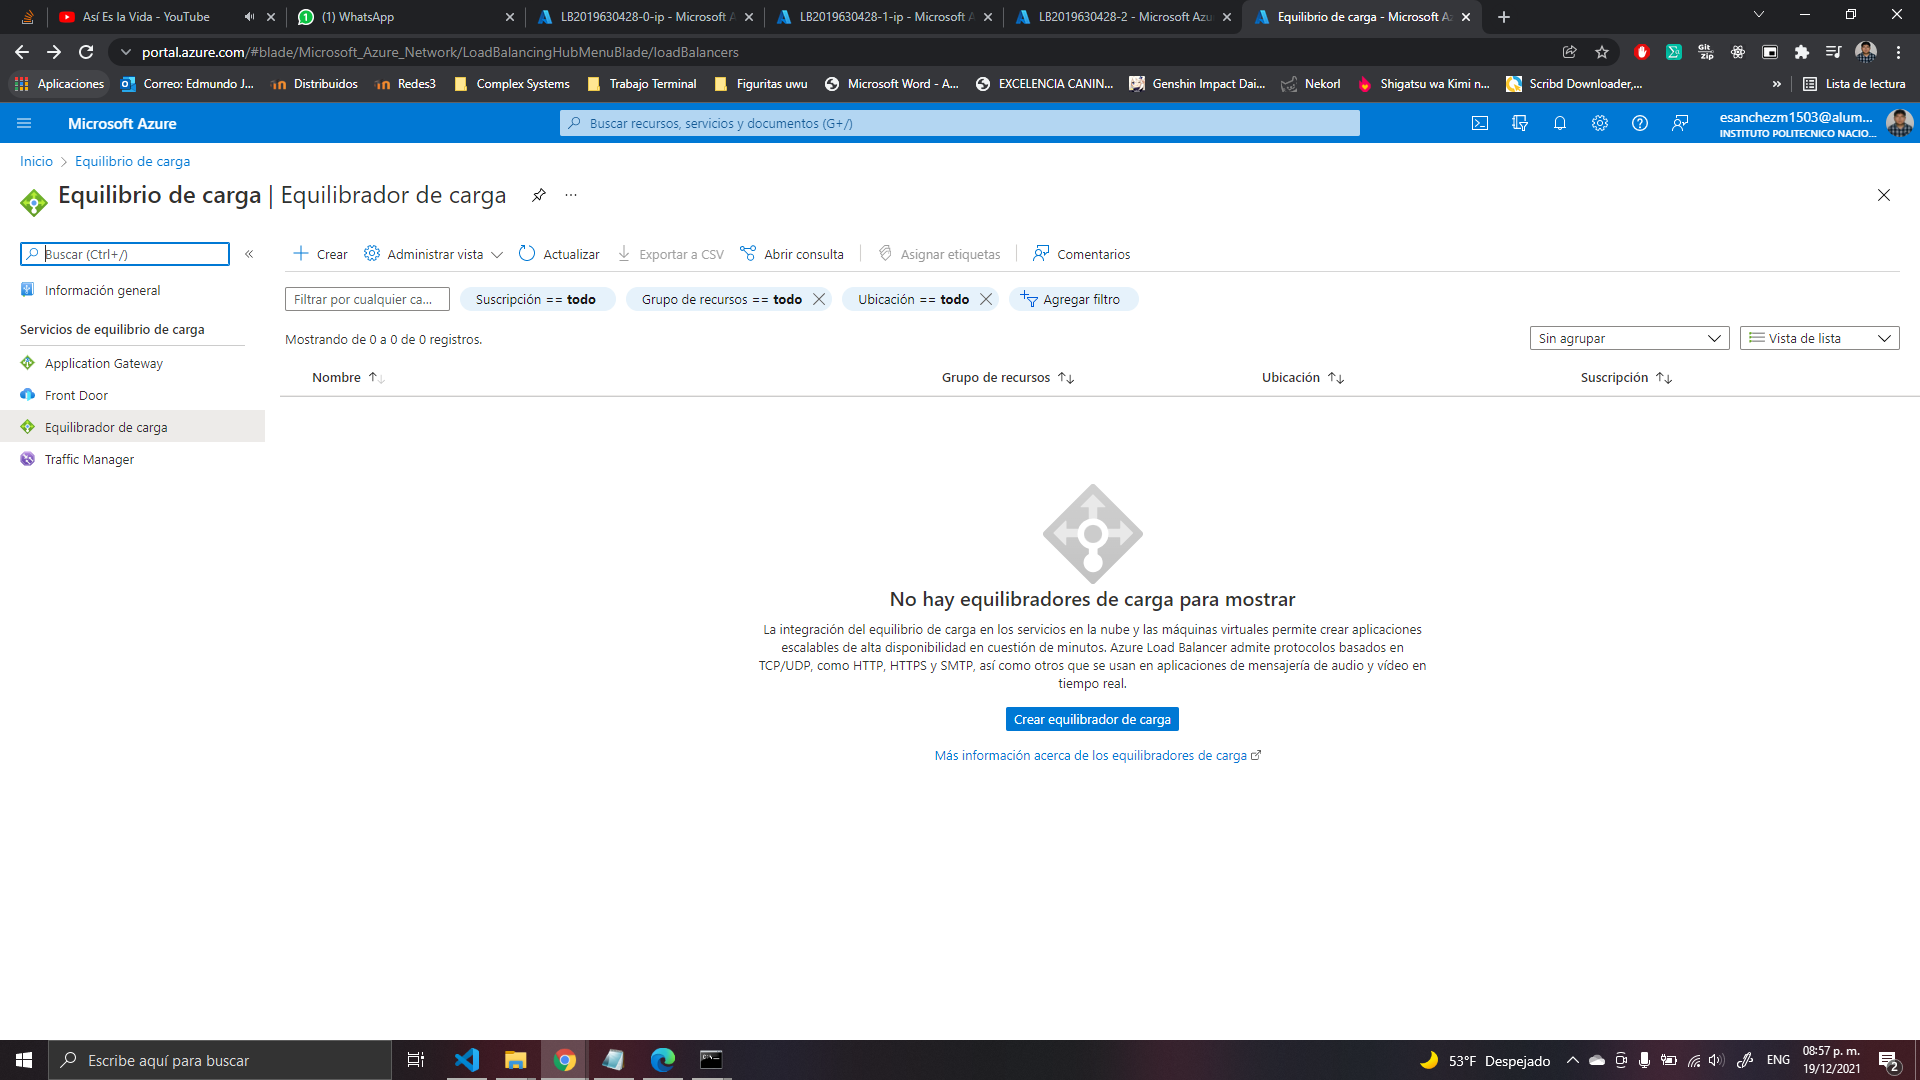
\includegraphics[scale=0.34]{resources/creacionBalanceador1-3.png}
				\caption{Opción de equilibrio de carga.}\label{fig:picture}
			\end{figure}
			\begin{figure}[H]
				\centering
				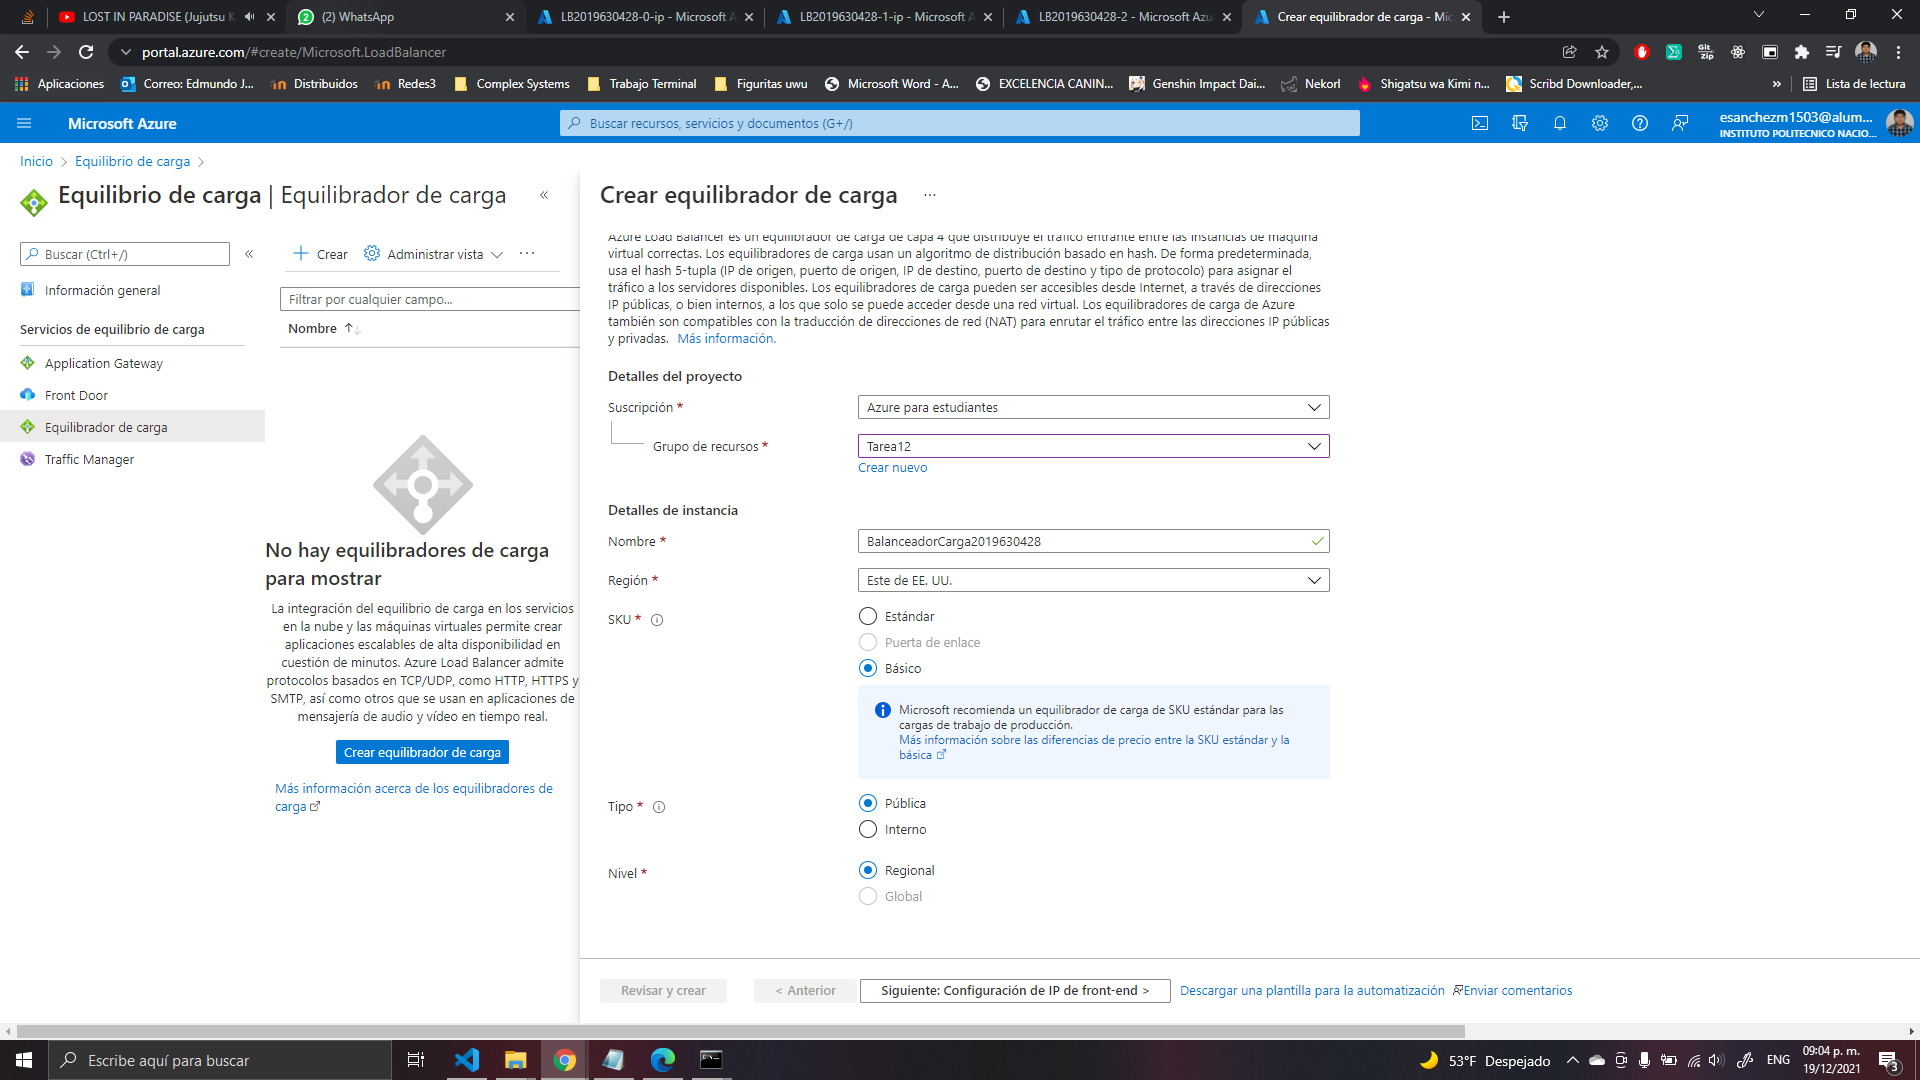
\includegraphics[scale=0.34]{resources/creacionBalanceador4-9.png}
				\caption{Creación de equilibrador de carga.}\label{fig:picture}
			\end{figure}
			Continuando con el proceso, seleccionamos la opción ``+Agregar una configuración de IP de front-end'' (Si aparece un error utilizar el navegador Edge.), ingresamos el nombre de la dirección IP pública y en el campo ``versión de IP'' seleccionamos ``IPv4'', en el campo ``Dirección de IP pública'' seleccionar ``Crear'', ingresamos el nombre de la IP pública, en el campo ``Asignación'' seleccionar ``Dinámica'' como vemos en la figura 36.
			\begin{figure}[H]
				\centering
				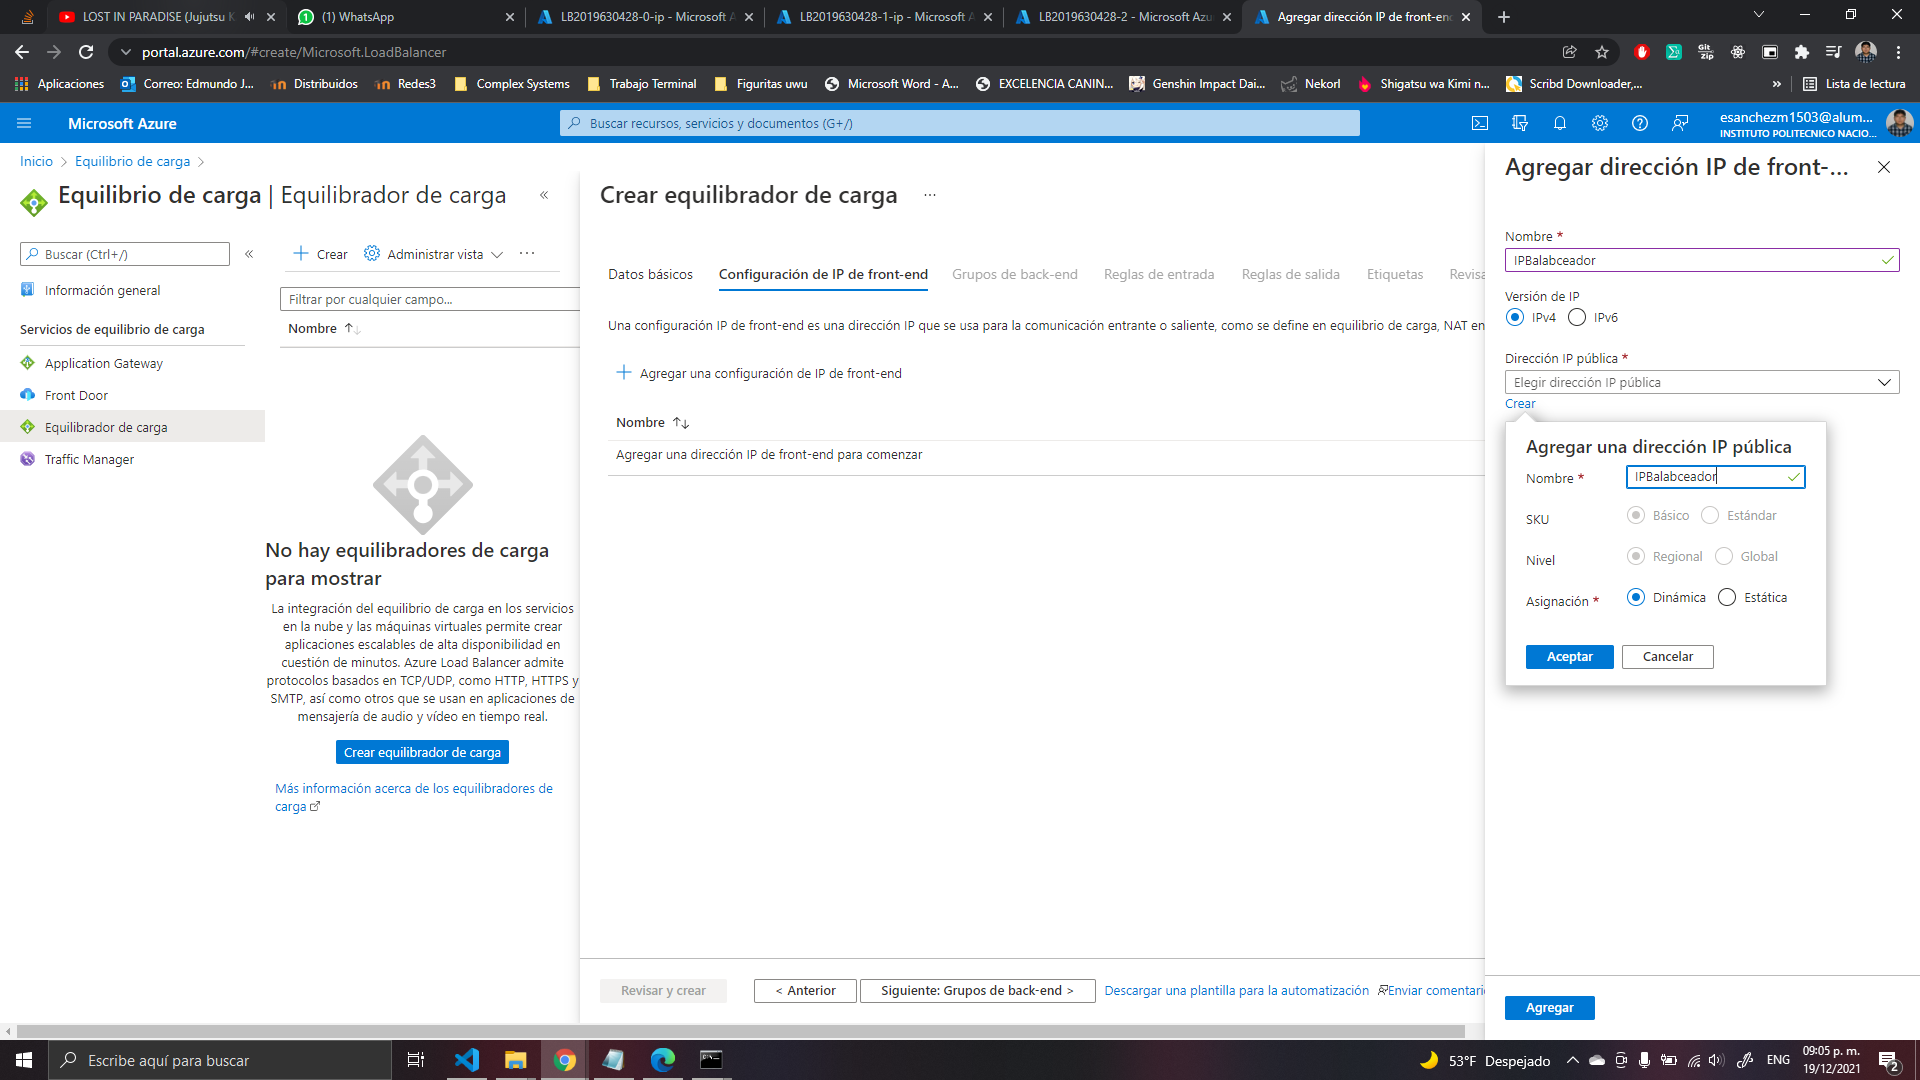
\includegraphics[scale=0.34]{resources/creacionBalanceador10-13.png}
				\caption{Configuración de IP de front-end.}\label{fig:picture}
			\end{figure}
			Finalmente en las figuras 37 y 38 vemos se añade la IP para el front-end y nos dice que esta por crearse y vemos la información general en la figura 38.
			\begin{figure}[H]
				\centering
				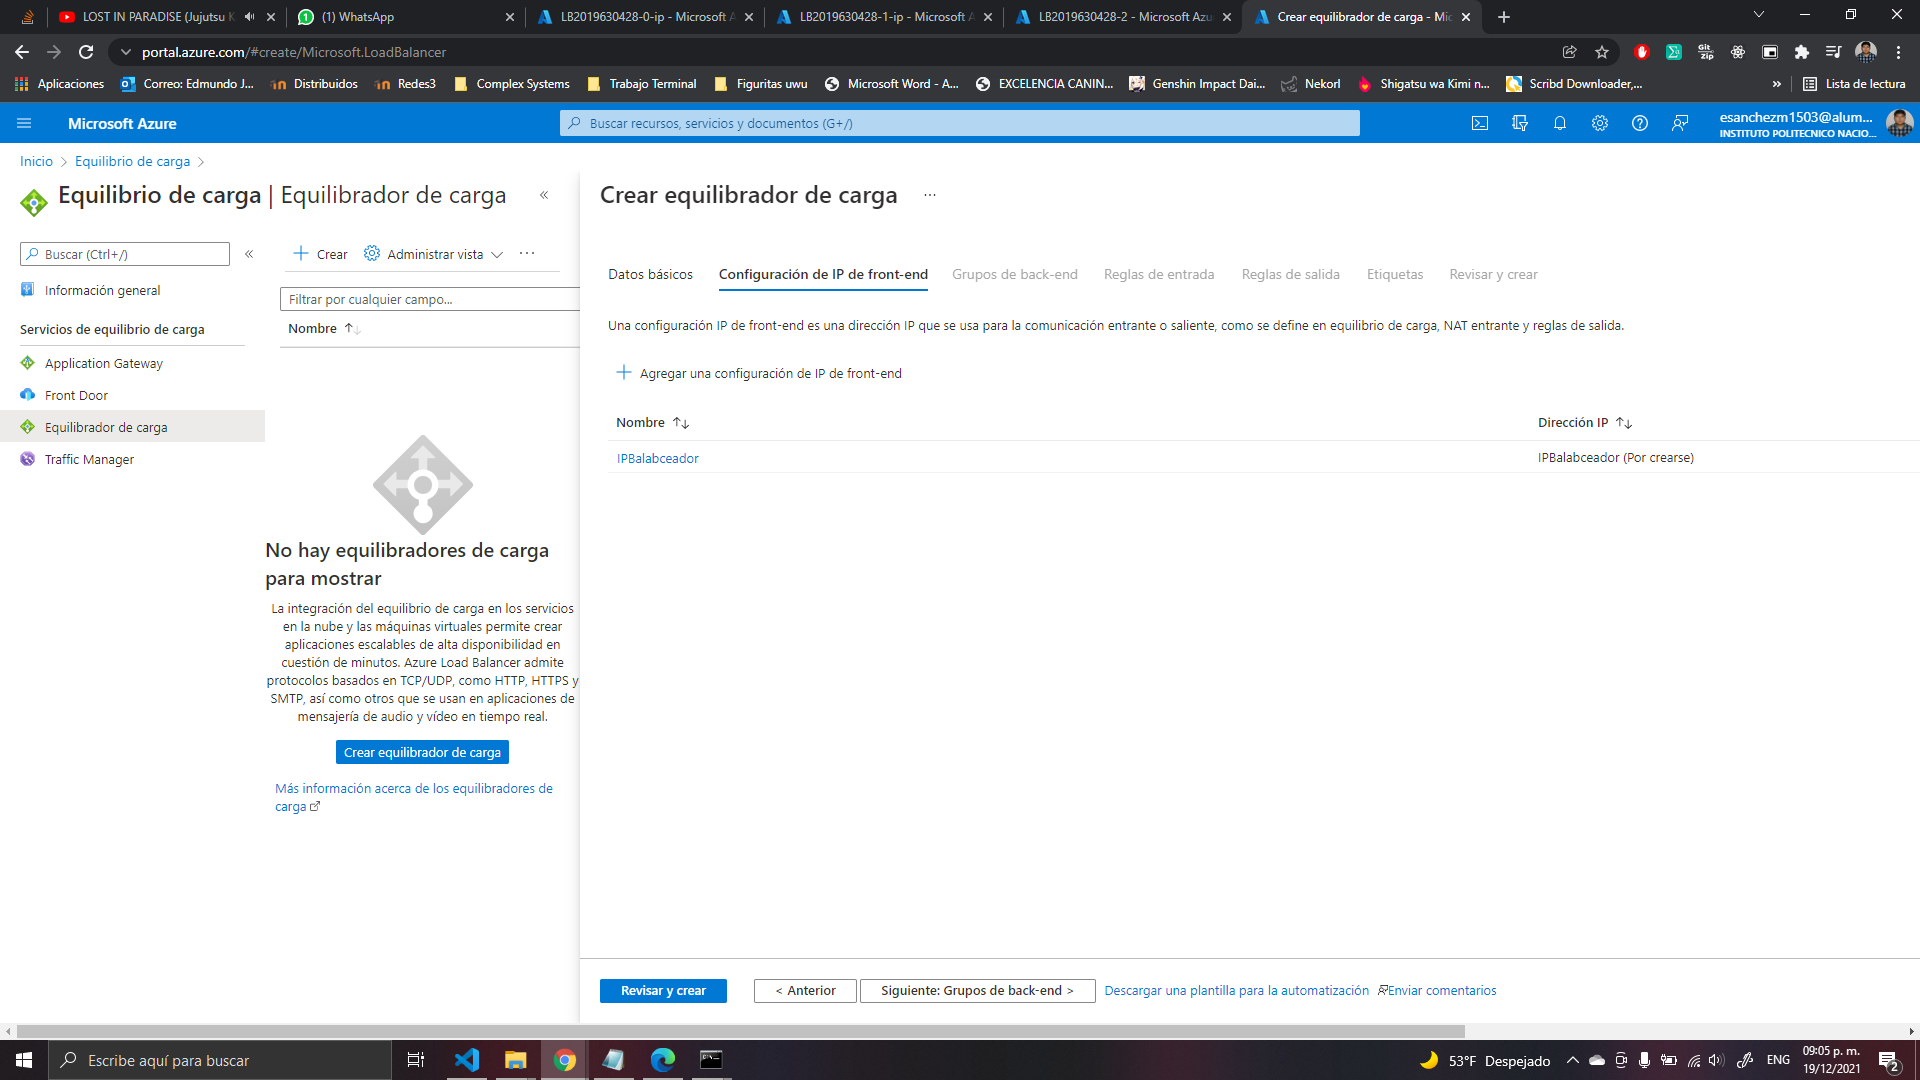
\includegraphics[scale=0.34]{resources/creacionBalanceador14-17.png}
				\caption{Información de la opción IP de front-end.}\label{fig:picture}
			\end{figure}
			\begin{figure}[H]
				\centering
				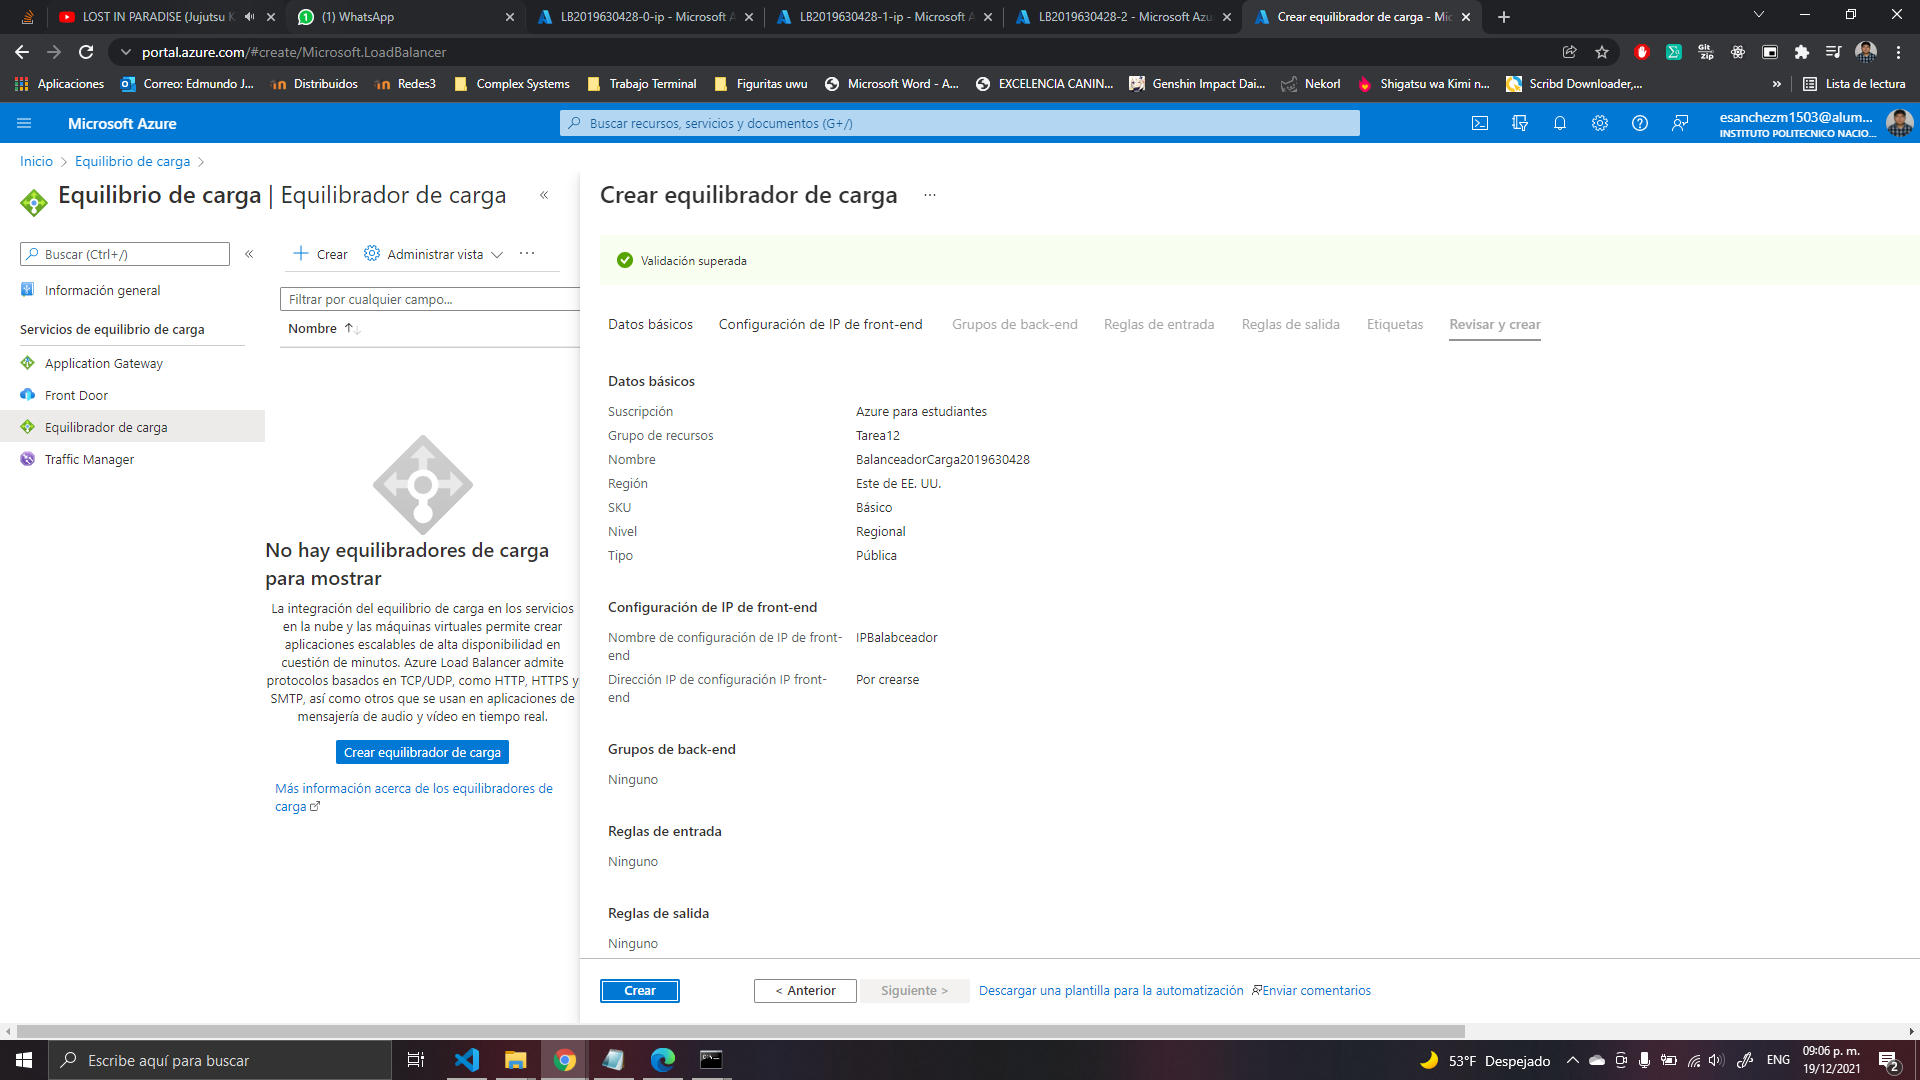
\includegraphics[scale=0.34]{resources/creacionBalanceador18.png}
				\caption{Revisar y crear.}\label{fig:picture}
			\end{figure}
			Finalmente vemos como se creo el balanceador de manera correcta en la figura 39.
			\begin{figure}[H]
				\centering
				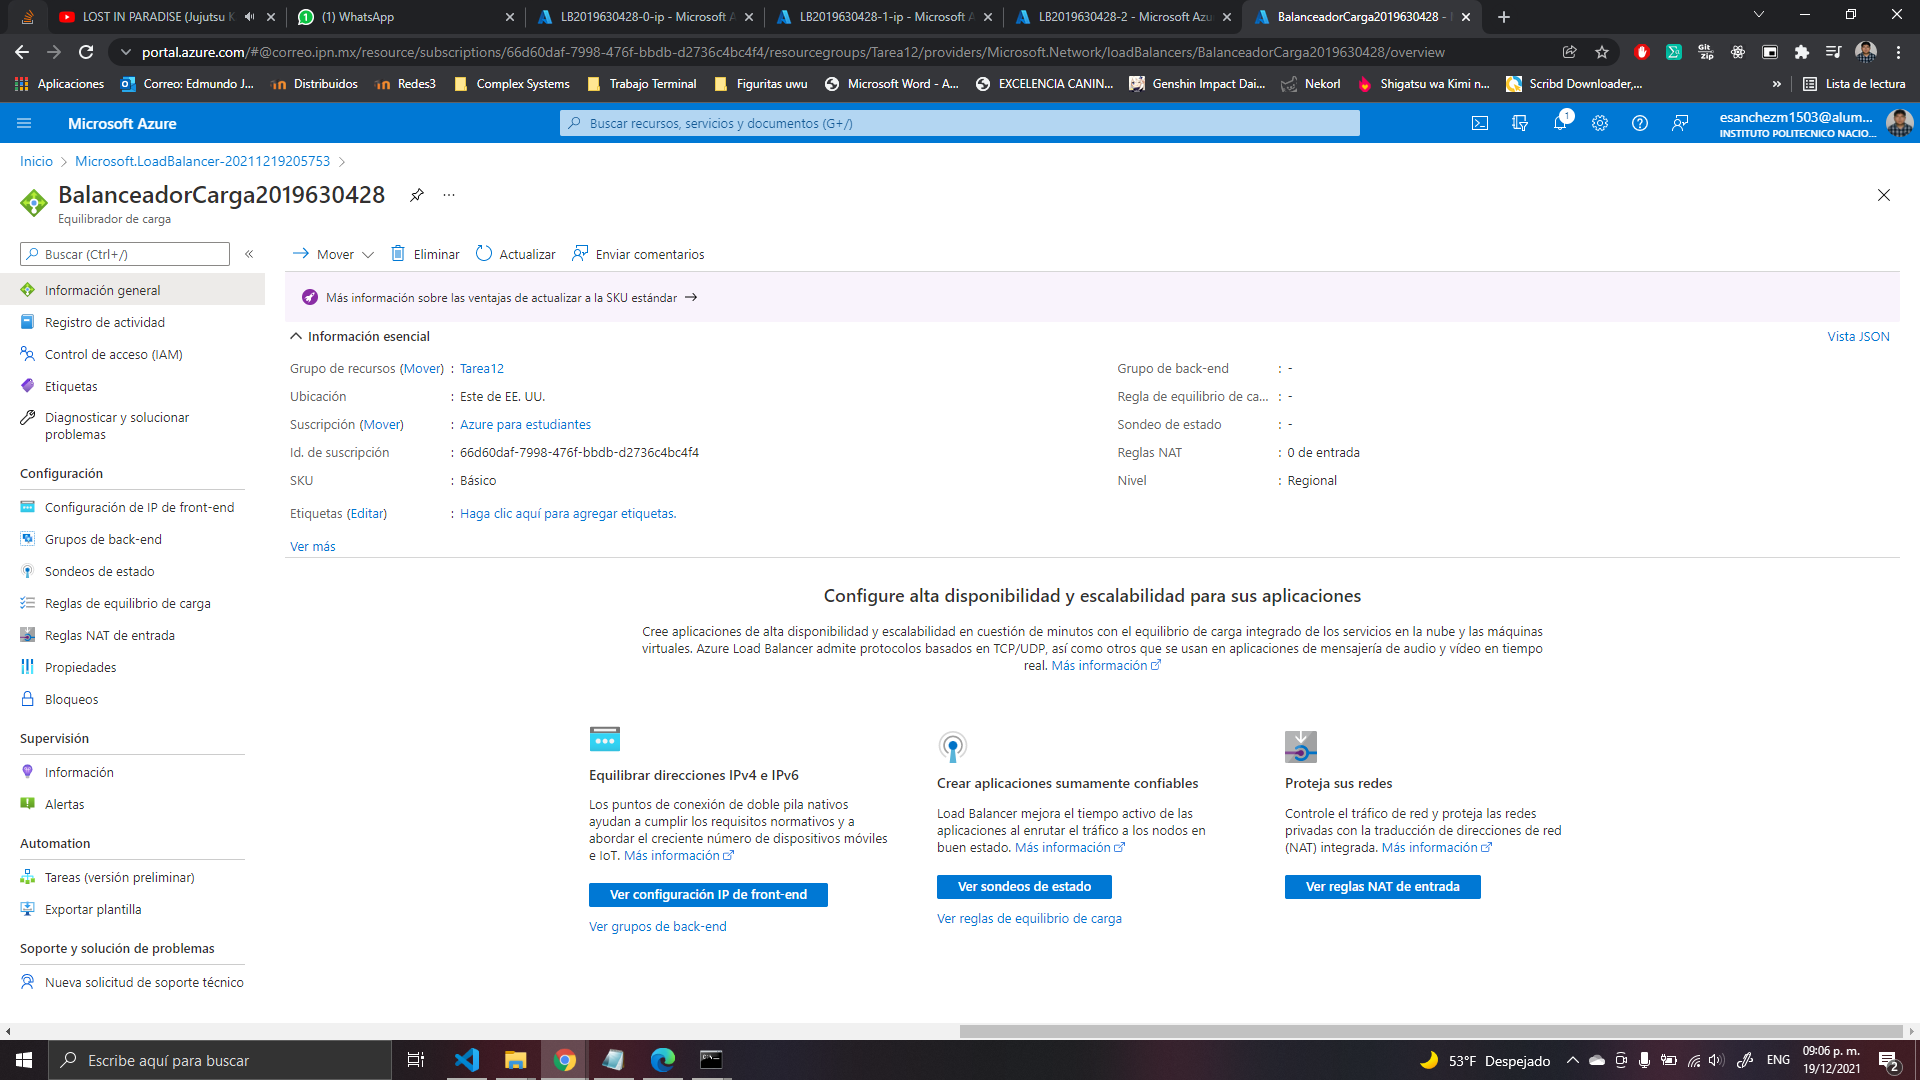
\includegraphics[scale=0.34]{resources/creacionBalanceadorF.png}
				\caption{Creación del balanceador exitosa.}\label{fig:picture}
			\end{figure}
			\subsubsection{Configuración del balanceador de carga}
			Ahora estando en el balanceador de carga, agregaremos máquinas virtuales al balanceador de carga para esto seleccionamos la opción ``Grupos de back-end'' en la sección ``Configuración'' del menú que aparece a la izquierda de la pantalla, como vemos en la figura 40. 
			\begin{figure}[H]
				\centering
				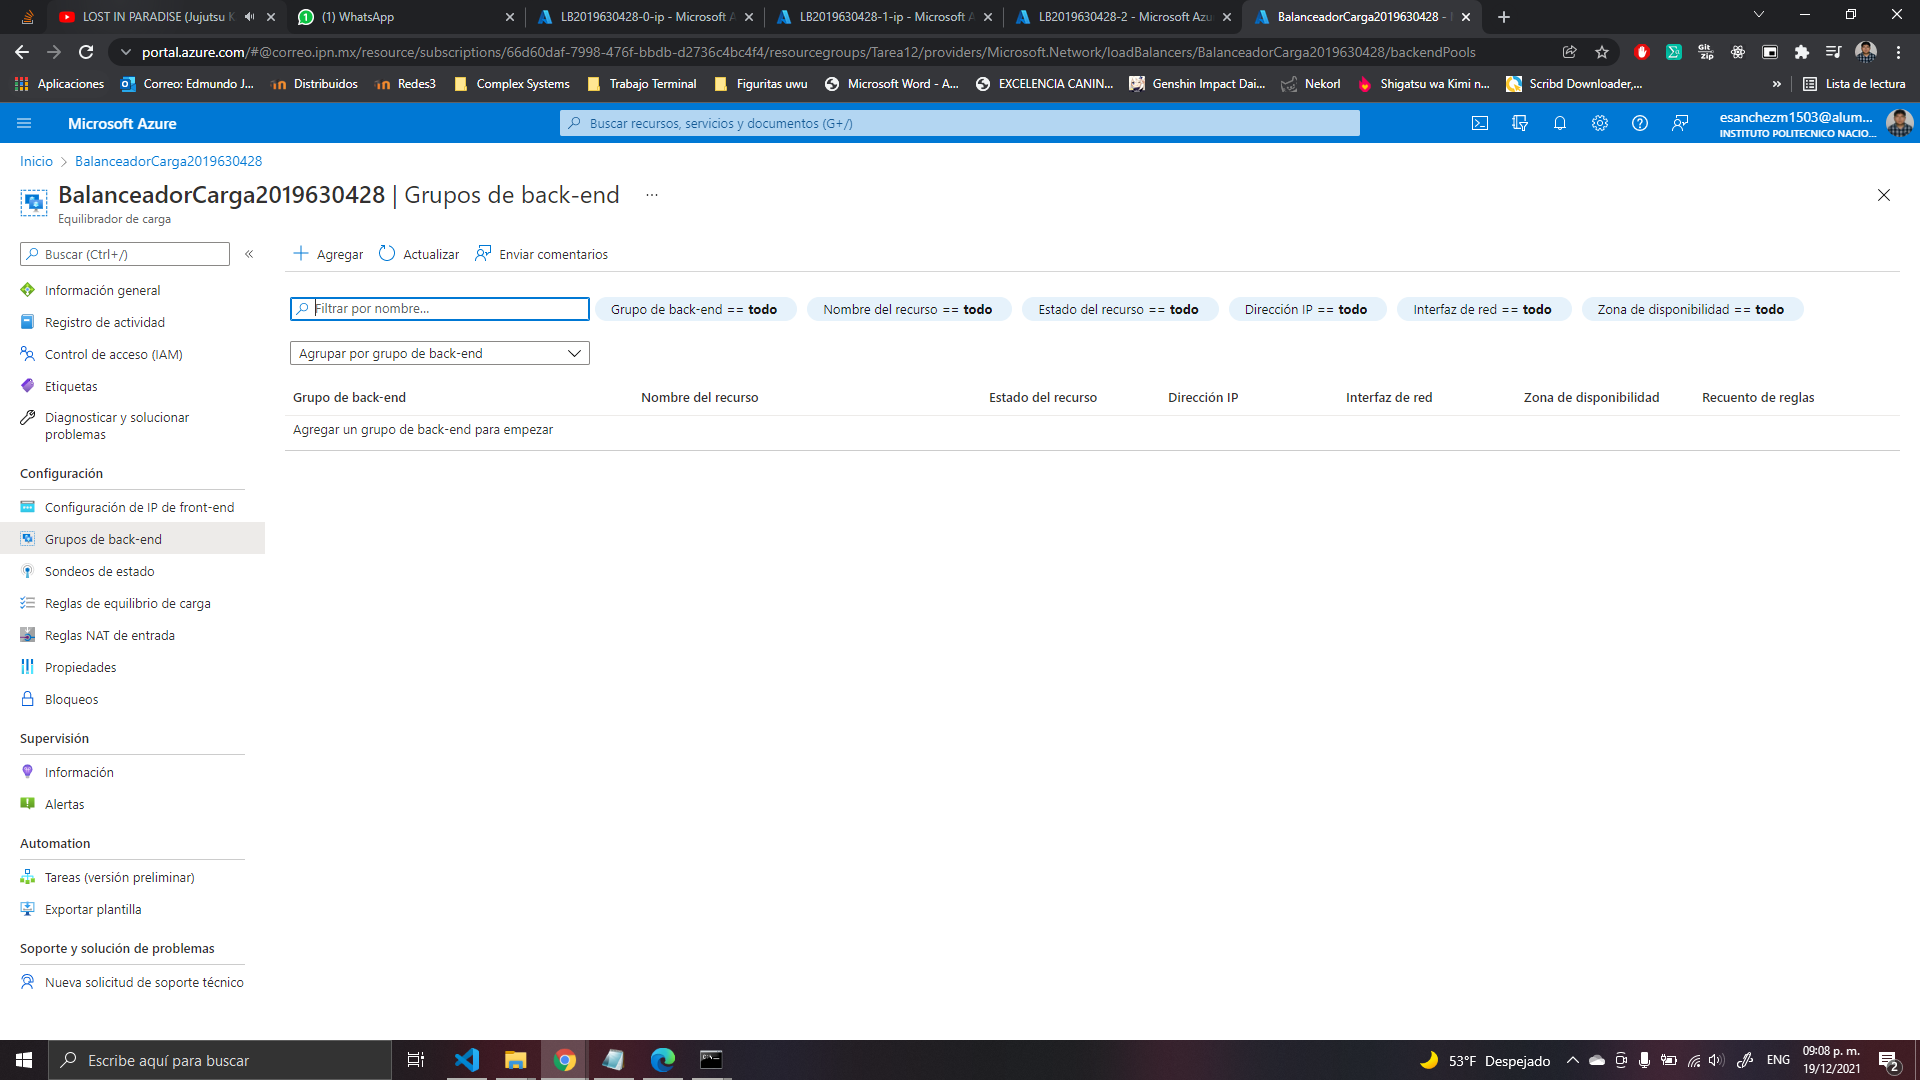
\includegraphics[scale=0.34]{resources/configBalanceador1-3.png}
				\caption{Opción grupos de back-end.}\label{fig:picture}
			\end{figure}
			Después seleccionamos la opción ``+Agregar'', ingresamos un nombre para el grupo de back-end, seleccionamos la red virtual donde están las máquinas virtuales, en el campo ``Asociado a'' seleccionar ``Maquinas virtuales'', seleccionamos la versión de IP: IPv4, damos clic al botón ``+Agregar'' para agregar una máquina virtual al grupo back-end. \textbf{Nota importante. Las máquinas virtuales no deben tener IP pública y deben estar en la misma ubicación y red virtual que el balanceador de carga. Al crear cada máquina virtual seleccionar ``Ninguno'' en el campo ``IP Pública'' en la pestaña ``Redes''.}, después marcamos la máquina virtual a agregar las cuales seran los nodos 0 y 1, damos clic al botón ``Agregar'', esto lo podemos ver en la figura 41 con los nodos 0 y 1 agregados al balanceador de carga.
			\begin{figure}[H]
				\centering
				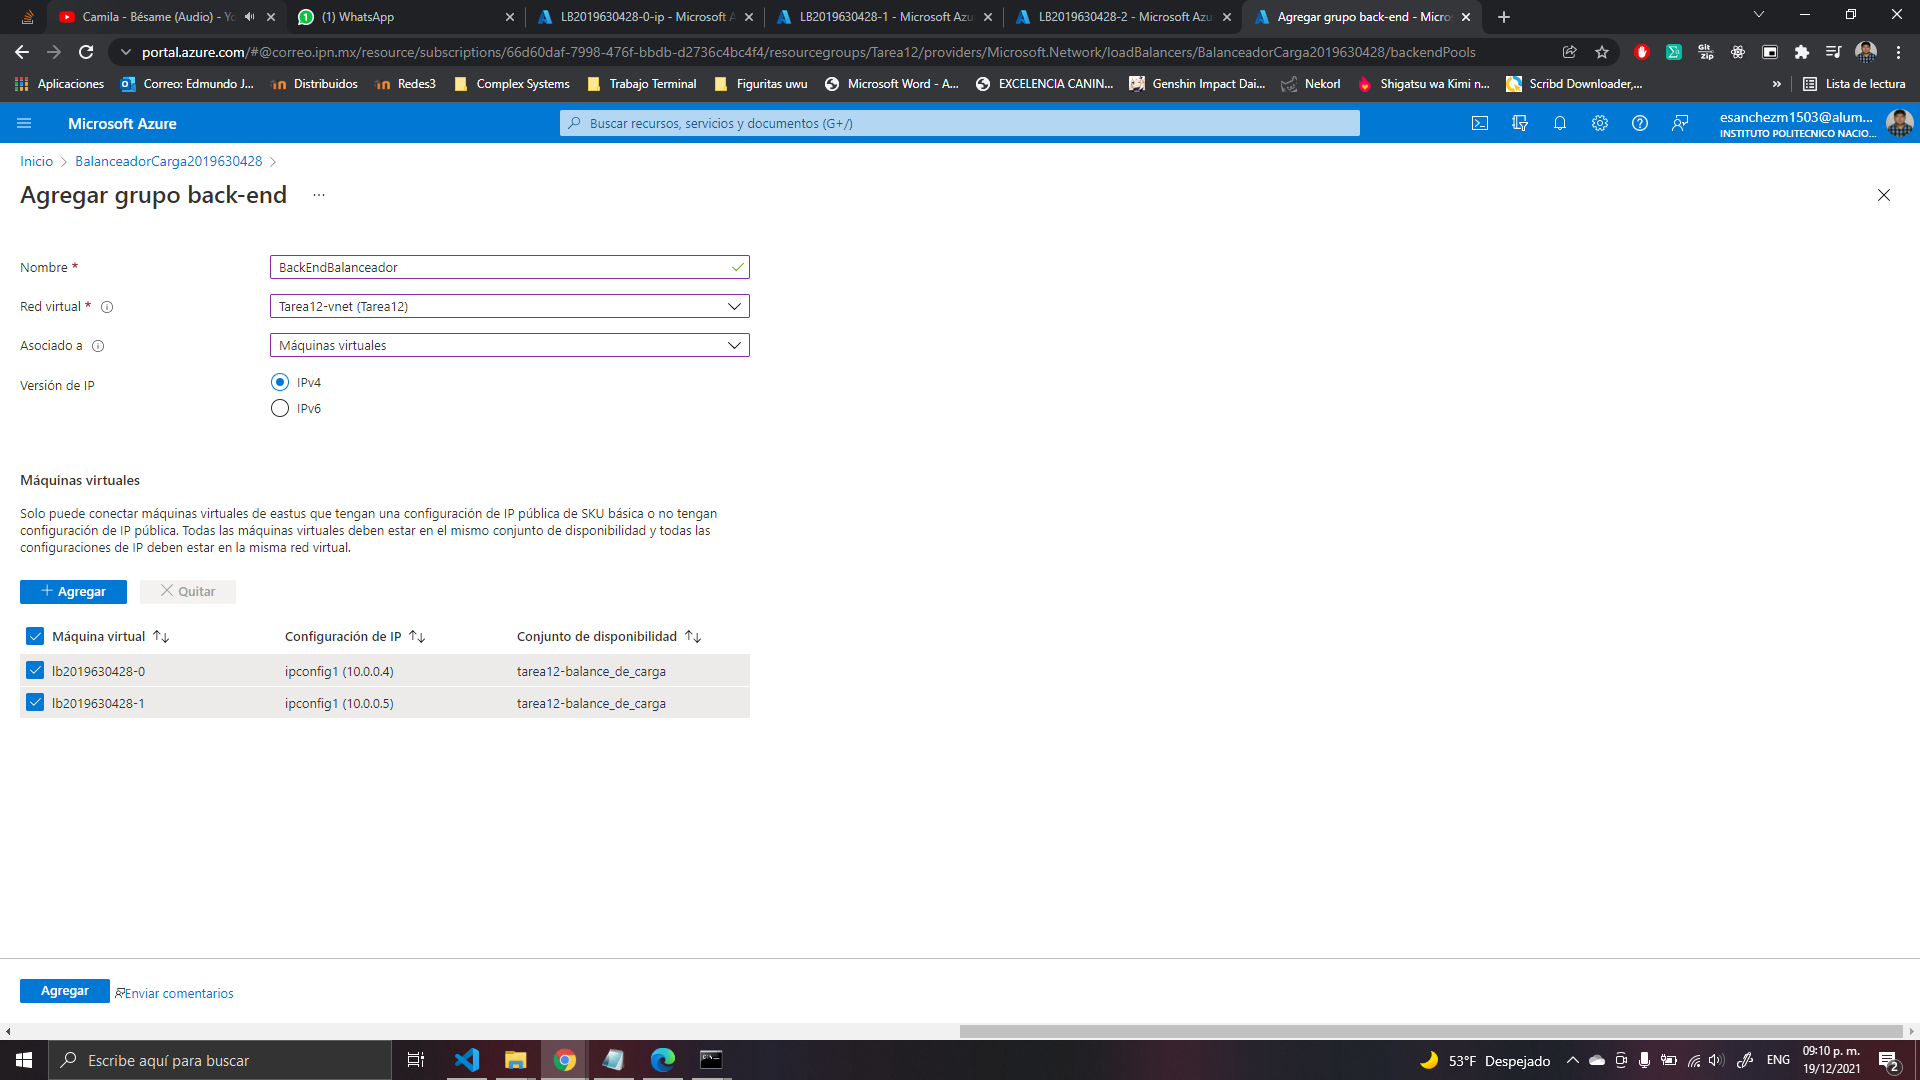
\includegraphics[scale=0.34]{resources/configBalanceador4-12.png}
				\caption{Maquinas agregadas al balanceador de carga.}\label{fig:picture}
			\end{figure}
			Finalmente damos clic al botón ``Agregar'' y vemos como en la figura 42 el procedimiento fue realizado de manera correcta.
			\begin{figure}[H]
				\centering
				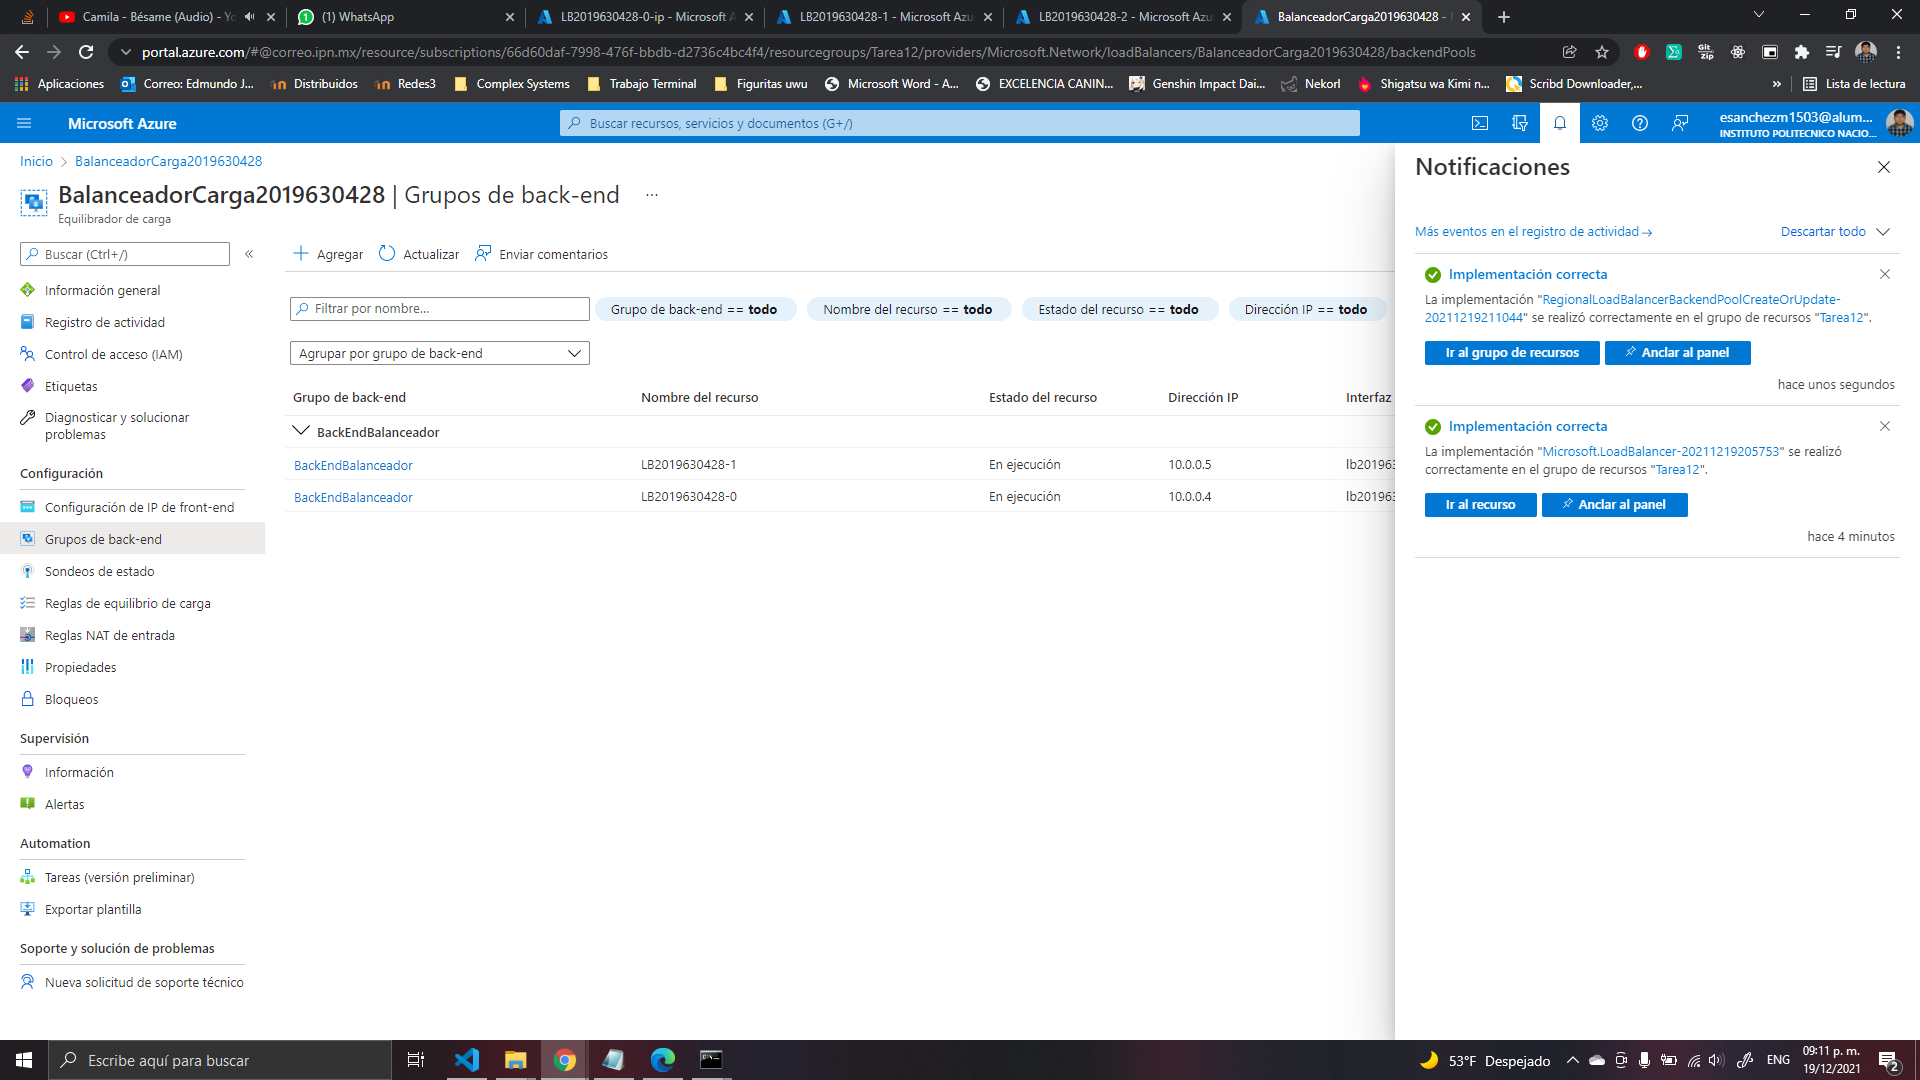
\includegraphics[scale=0.34]{resources/configBalanceadorF.png}
				\caption{Maquinas agregadas al balanceador de carga de manera correcta.}\label{fig:picture}
			\end{figure}
			\subsubsection{Agregar un sondeo de estado}
			Antes de agregar reglas de equilibrio de carga es necesario crear al menos un sondeo de estado, ahora iremos a la opción ``Sondeos de estado'' en la sección ``Configuración'' del menú que aparece a la izquierda de la pantalla como vemos en la figura 43.
			\begin{figure}[H]
				\centering
				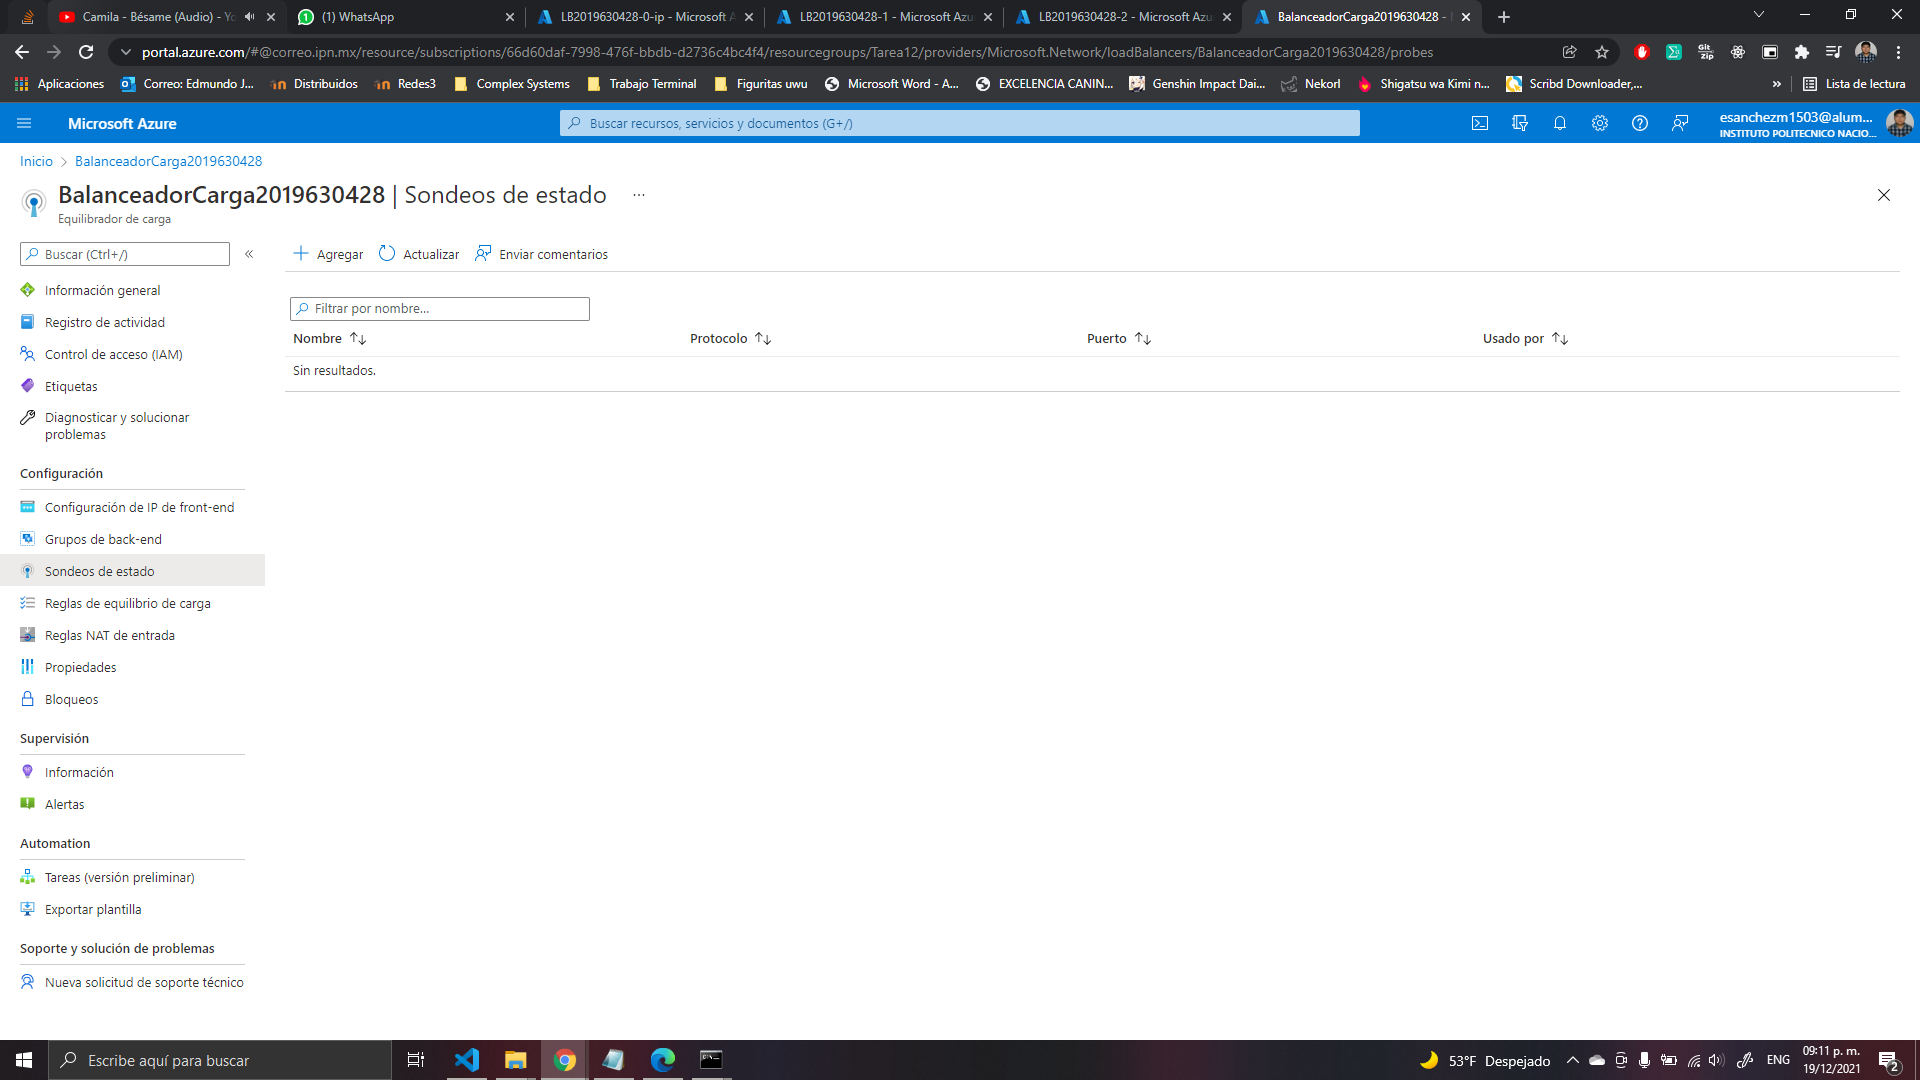
\includegraphics[scale=0.34]{resources/sondeoBalanceador1-3.png}
				\caption{Opción sondeos de estado.}\label{fig:picture}
			\end{figure}
			Ahora seleccionamos la opción ``+Agregar'', ingresamos el nombre del sondeo, seleccionamos el protocolo: TCP, ingresamos el puerto que se sondeará: 8080, ingresamos el intervalo de sondeo en segundos, ingresar el umbral incorrecto (número de errores de sondeo consecutivos que indican que el estado de la máquina virtual no es correcto) y damos clic en el botón "Aceptar" como vemos en la figura 44. \textbf{Nota. Se deberá abrir el puerto 8080 en cada máquina virtual para que se pueda hacer el sondeo de estado.}
			\begin{figure}[H]
				\centering
				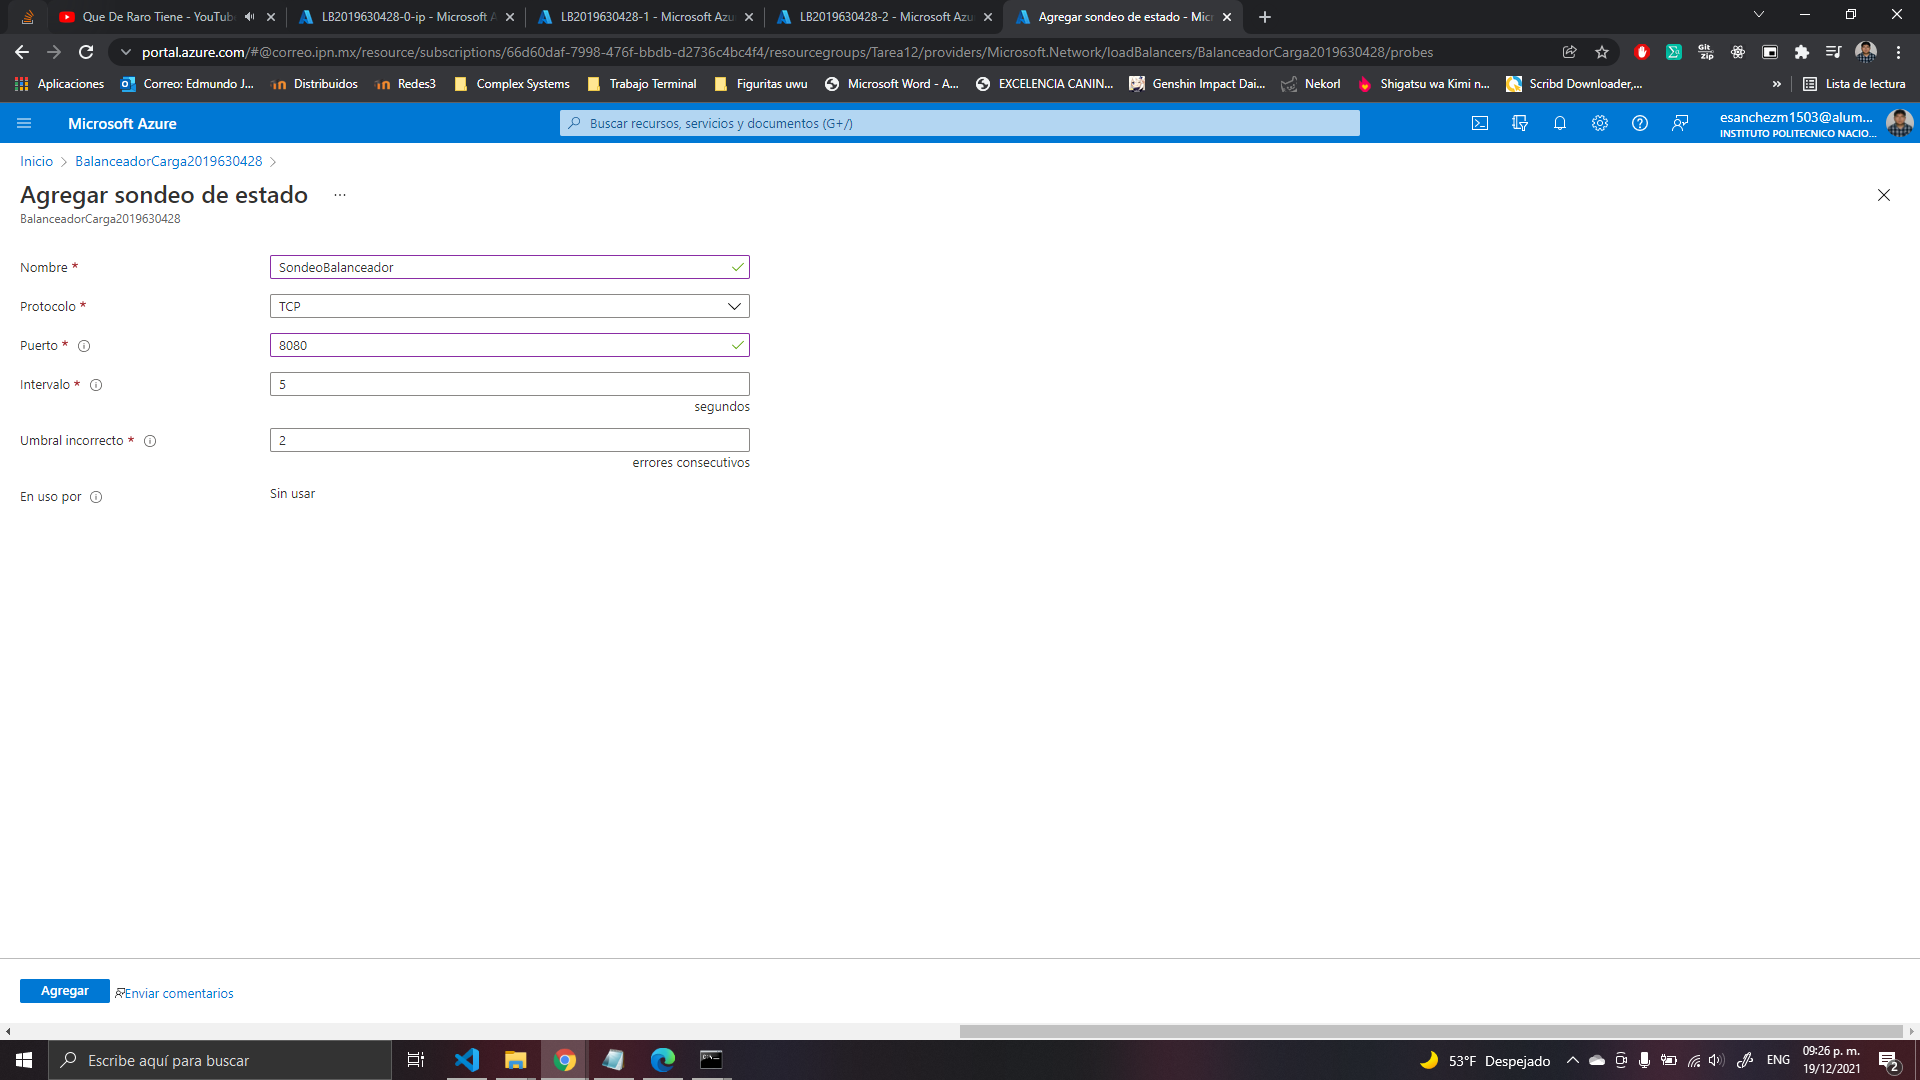
\includegraphics[scale=0.34]{resources/sondeoBalanceador4-9.png}
				\caption{Creación de sondeo de estado.}\label{fig:picture}
			\end{figure}
			Si vemos la figura 45 podemos ver como el sondeo de estado fue creado de manera correcta.
			\begin{figure}[H]
				\centering
				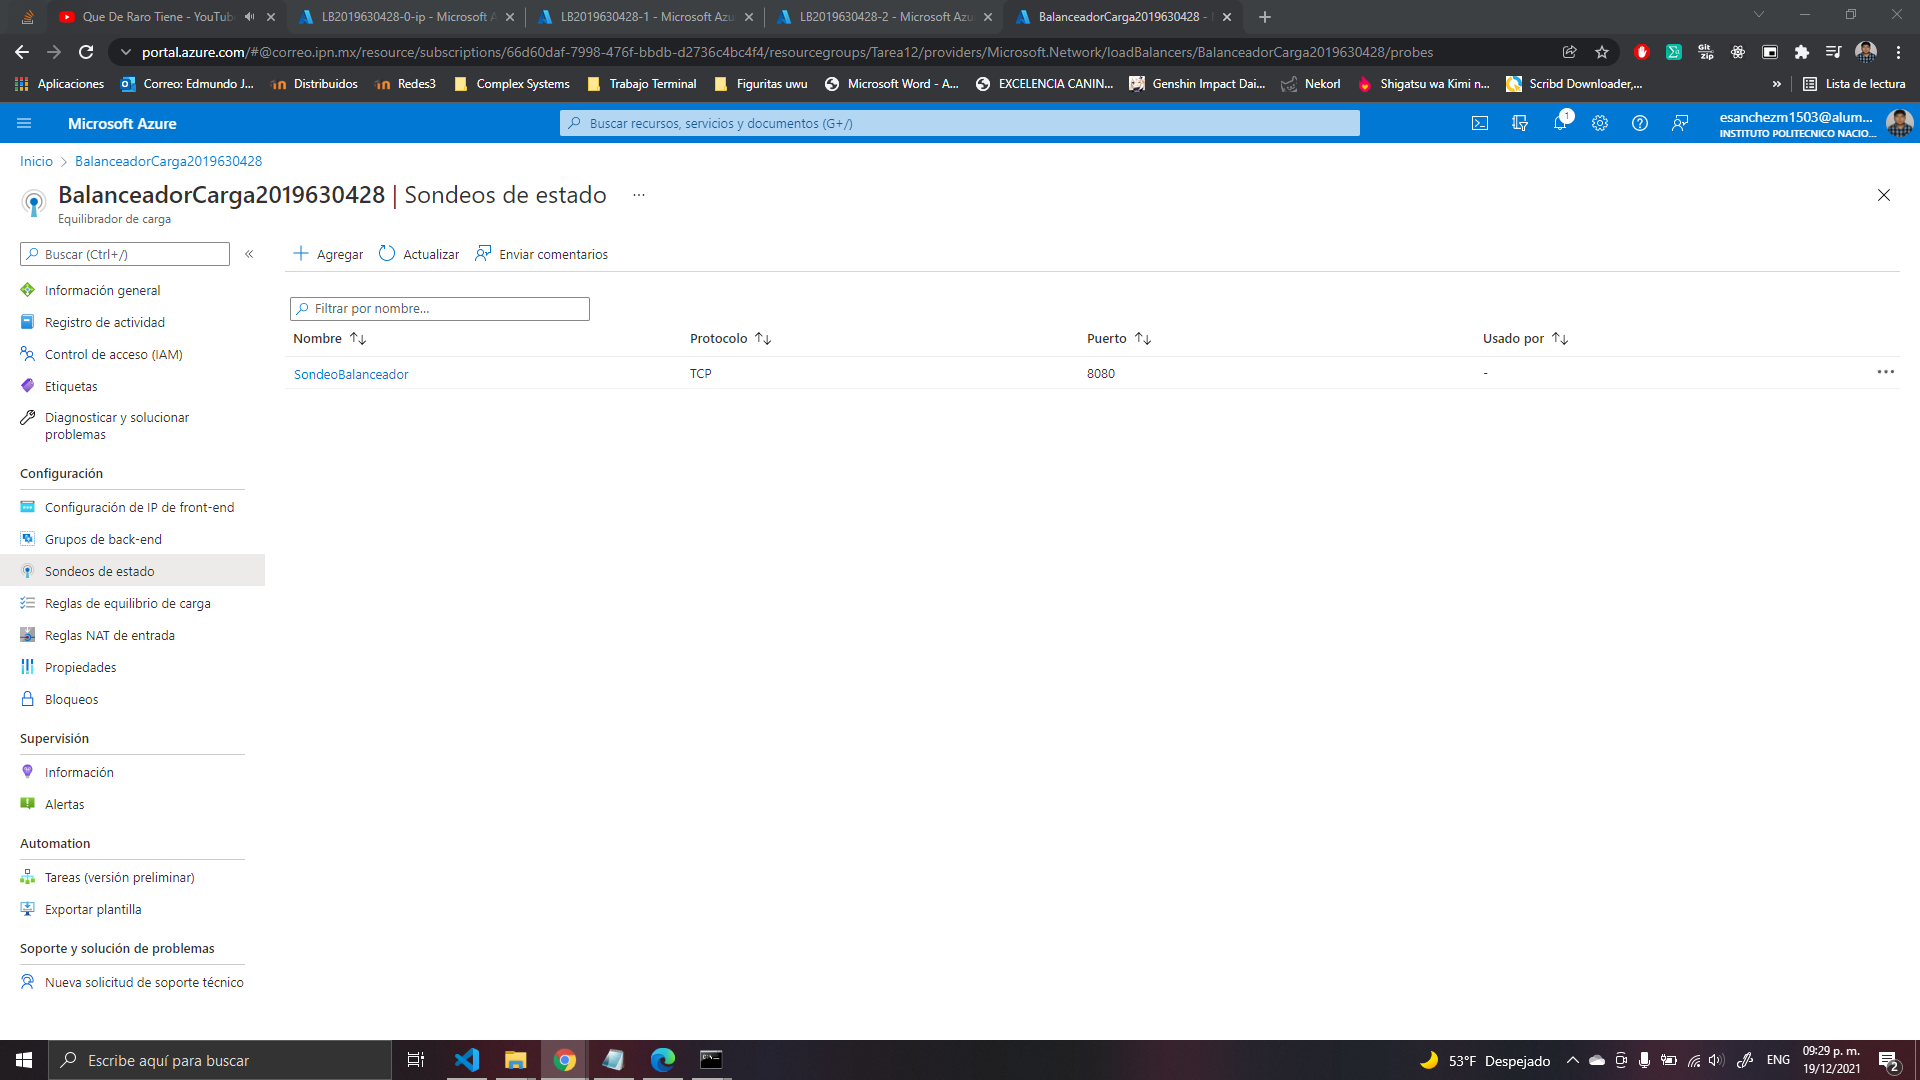
\includegraphics[scale=0.34]{resources/sondeoBalanceadorF.png}
				\caption{Creación de sondeo de estado correcto.}\label{fig:picture}
			\end{figure}
			\subsubsection{Agregar una regla de equilibrio de carga}
			Finalmente iremos a la opción ``Reglas de equilibrio de carga'' como vemos en la figura 46.
			\begin{figure}[H]
				\centering
				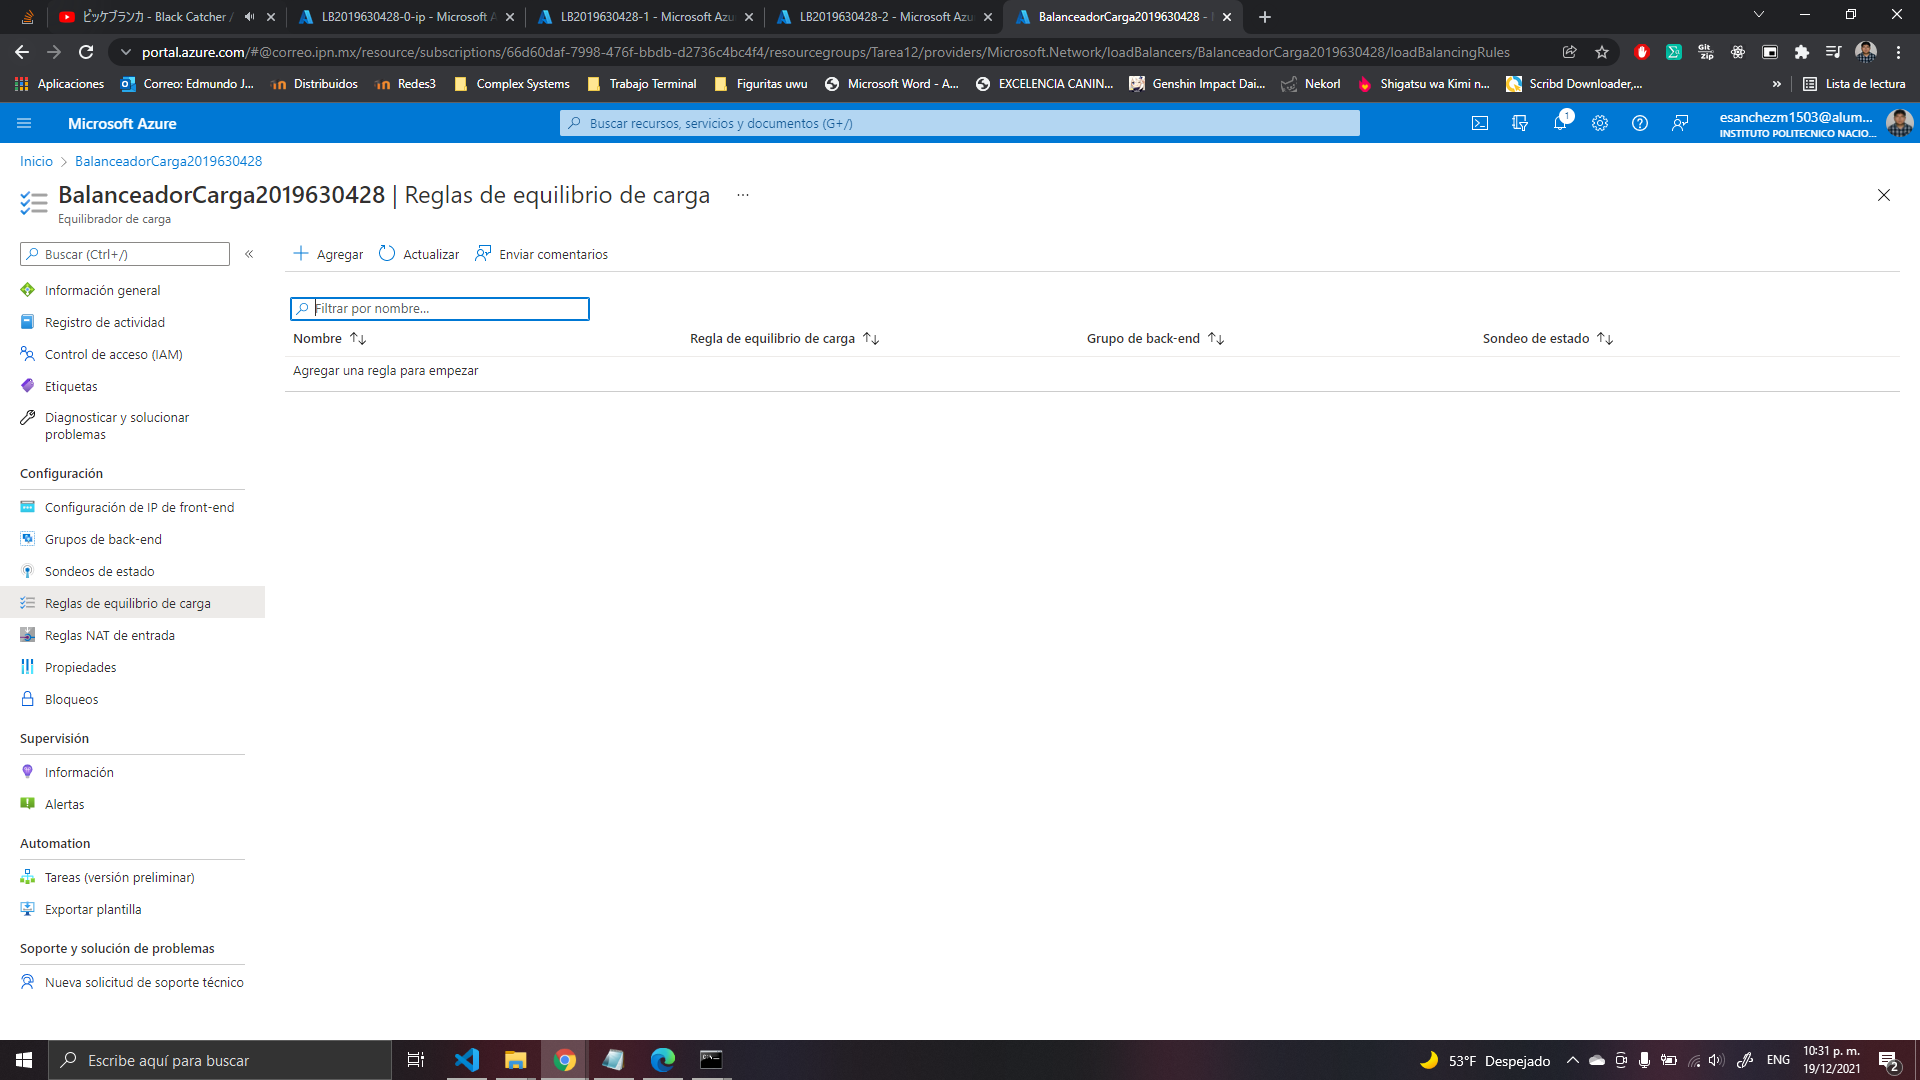
\includegraphics[scale=0.34]{resources/reglaBalanceador1-3.png}
				\caption{Opción reglas de equilibrio de carga.}\label{fig:picture}
			\end{figure}
			Ingresamos el nombre de la regla, seleccionamos la versión de IP: IPv4, seleccionamos la dirección IP de fron-end (la IP del balanceador de carga), seleccionamos el Grupo de back-end (previamente creado), seleccionamos el protocolo: TCP, ingresamos el puerto (del balanceador de carga), por ejemplo: 80, ingresamos el puerto de back-end, por ejemplo: 8080

El puerto en las máquinas virtuales podría ser diferente al puerto que usan los clientes para conectarse con el balanceador de carga. Este puerto deberá estar abierto en todas las máquinas virtuales dentro del grupo back-en.
Finalmente seleccionamos el sondeo de estado (previamente creado), todo lo anterior lo podemos ver en al figura 47 y damos clic en el botón ``Aceptar'' y vemos como en la figura 48 se creo de manera exitosa.
			\begin{figure}[H]
				\centering
				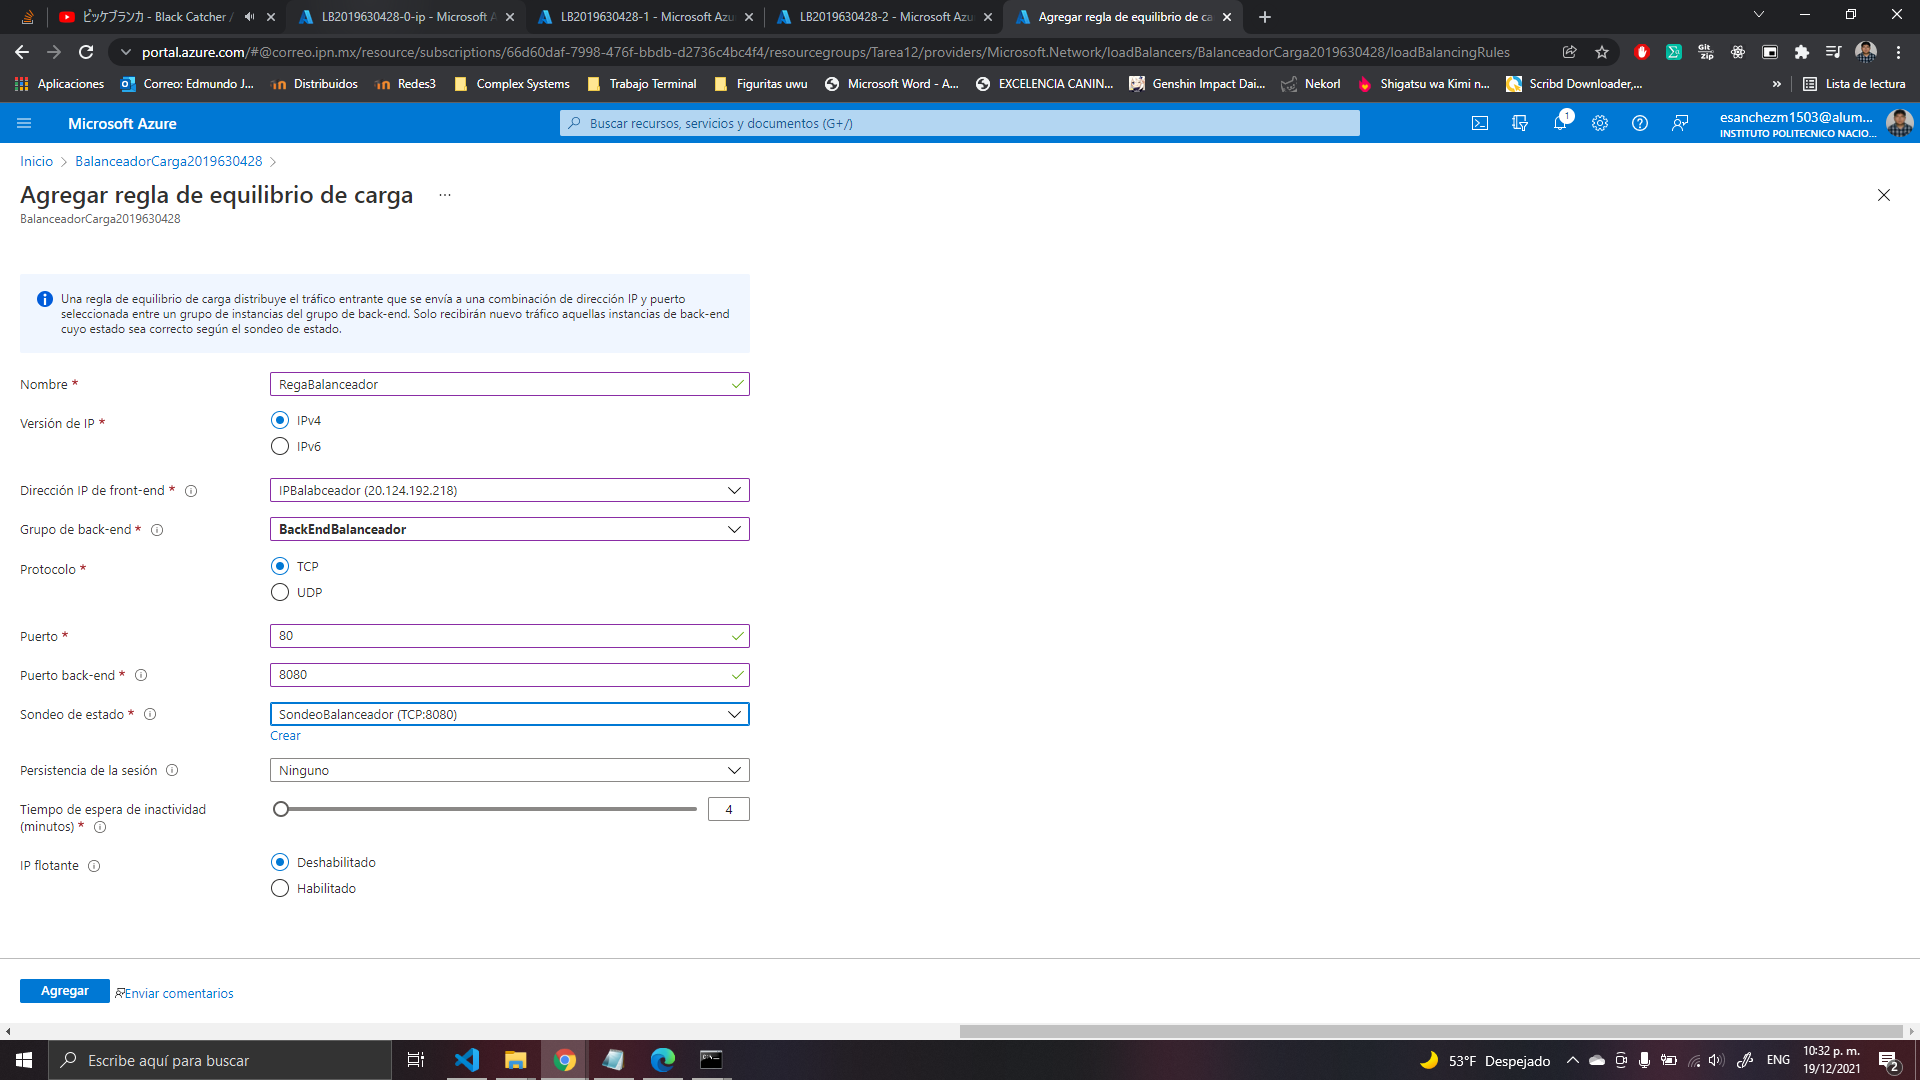
\includegraphics[scale=0.34]{resources/reglaBalanceador4-12.png}
				\caption{Creación de reglas de equilibrio de carga.}\label{fig:picture}
			\end{figure}
			\begin{figure}[H]
				\centering
				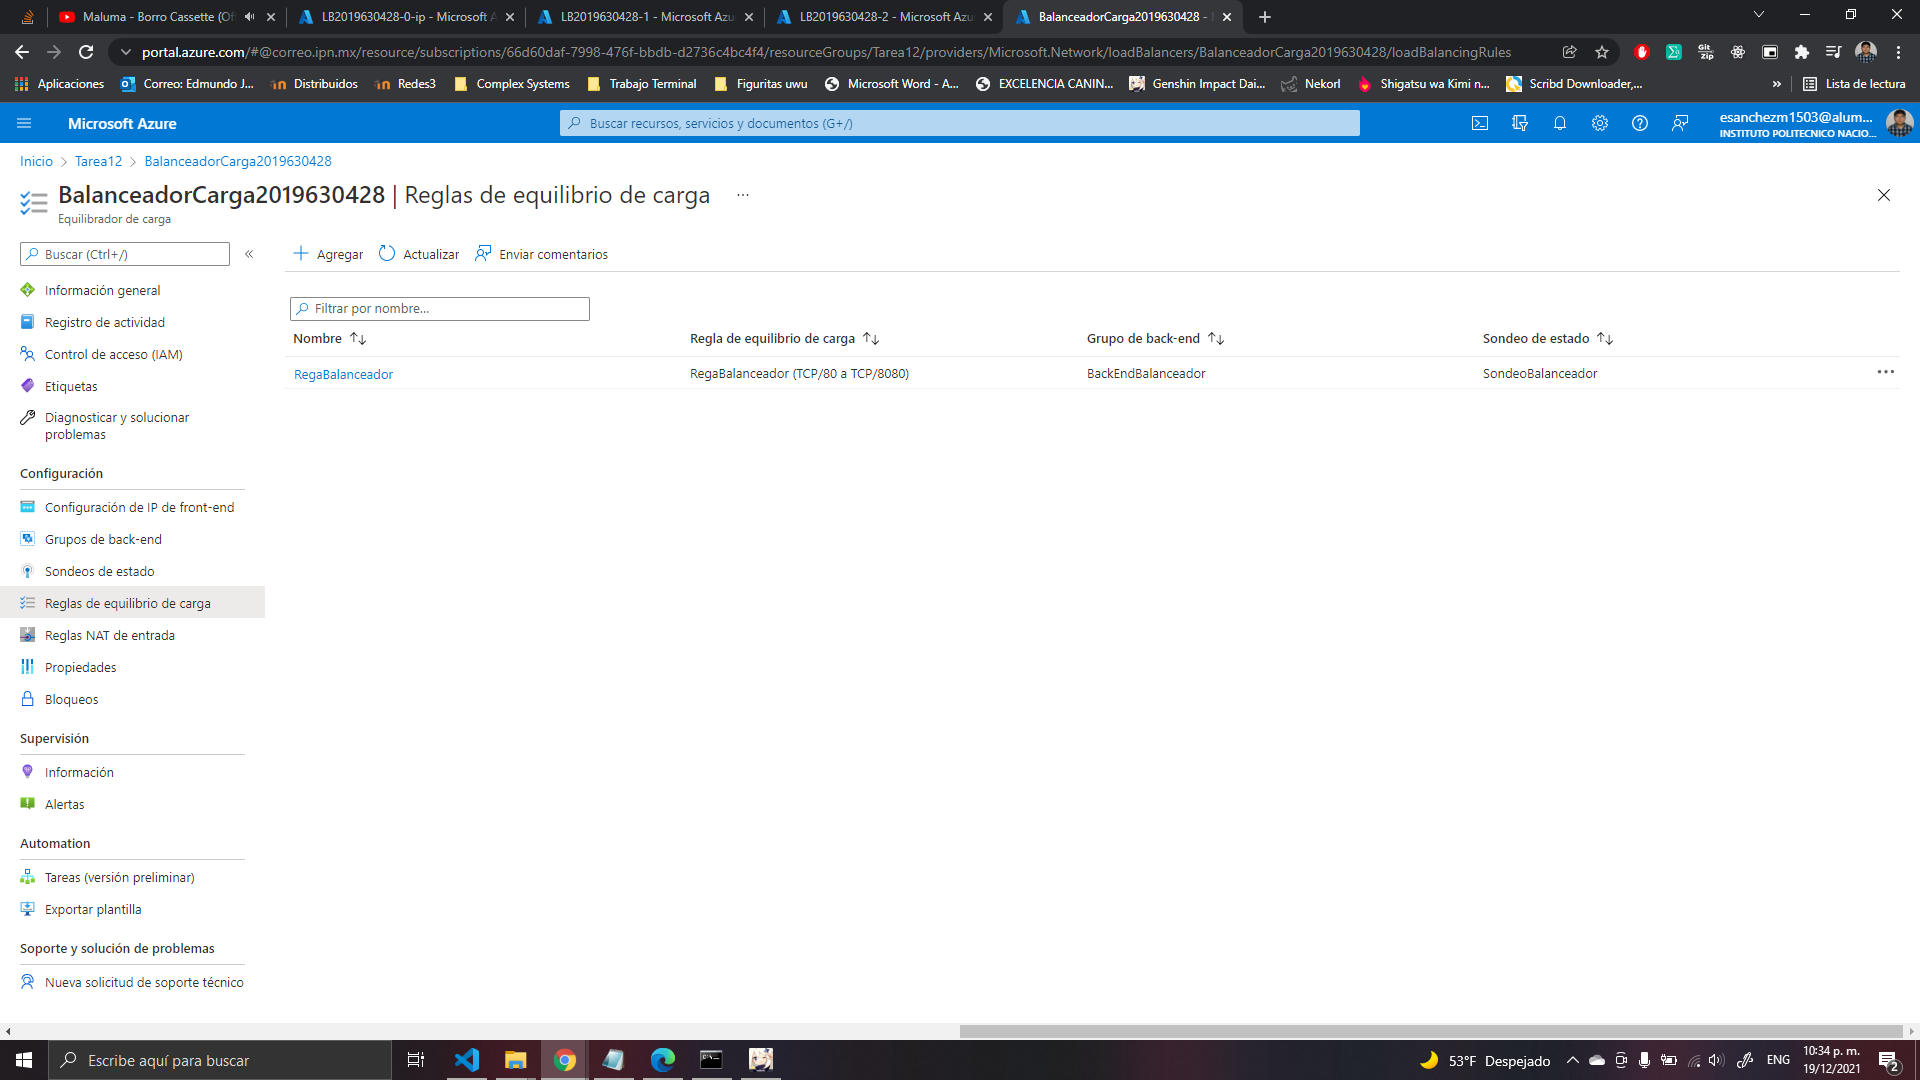
\includegraphics[scale=0.34]{resources/reglaBalanceadorF.png}
				\caption{Creación de reglas de equilibrio de carga correcto.}\label{fig:picture}
			\end{figure}
			Estos son todos los pasos que se tienen que hacer para la creación de nuestro balanceador de carga, ahora pasemos a las pruebas. 
			
		\subsection{Pruebas}
		Antes de todo veamos el estado de base de datos como vemos en la figura 49.
		\begin{figure}[H]
				\centering
				\includegraphics[scale=0.34]{resources/estadoDB.png}
				\caption{Estado de la base de datos.}\label{fig:picture}
		\end{figure}
		Ahora vayamos netamente a las pruebas. Para empezar nos dirigiremos a la URL http://20.124.192.218/prueba.html (ver figura 50) la cual es la IP del balanceador de carga esto para cargar una pagina HTML en la cual podemos hacer el clásico ABCC, es decir altas, bajas, cambios y consultas de una base de datos. Empecemos así con una alta, para esto veamos la figura 51 vemos los datos que serán dados de alta y en la figura 52 vemos el mensaje de que el usuario se dio de alta y vemos como en la figura 53 el alto se realizo de manera correcta.
		\begin{figure}[H]
			\centering
			\includegraphics[scale=0.34]{resources/prueba1.png}
			\caption{Pagina prueba.html.}\label{fig:picture}
		\end{figure}
		\begin{figure}[H]
			\centering
			\includegraphics[scale=0.34]{resources/prueba2.1.png}
			\caption{Alta de usuario.}\label{fig:picture}
		\end{figure}
		\begin{figure}[H]
			\centering
			\includegraphics[scale=0.34]{resources/prueba2.2.png}
			\caption{Alta de usuario correcto.}\label{fig:picture}
		\end{figure}
		\begin{figure}[H]
			\centering
			\includegraphics[scale=0.34]{resources/prueba2.3.png}
			\caption{Cambio en la base de datos después del registro.}\label{fig:picture}
		\end{figure}
		La siguiente prueba sera dar de alta un usuario con el mismo correo que se ocupo, como vemos nos regresa un mensaje diciendo que el email ya existe como se ve en la figura 54.
		\begin{figure}[H]
			\centering
			\includegraphics[scale=0.34]{resources/prueba3.2.png}
			\caption{Alta de usuario con el mismo correo.}\label{fig:picture}
		\end{figure}
		Una prueba mas sera la de consultar un usuario por medio del correo electrónico como vemos en la figura 55 solo colocamos el correo electrónico que se registro y como vemos en la figura 56 nos muestra la información que registramos en la figura 51.
		\begin{figure}[H]
			\centering
			\includegraphics[scale=0.34]{resources/prueba4.1.png}
			\caption{Consulta por medio del correo.}\label{fig:picture}
		\end{figure}
		\begin{figure}[H]
			\centering
			\includegraphics[scale=0.34]{resources/prueba4.2.png}
			\caption{Resultado de la consulta anterior.}\label{fig:picture}
		\end{figure}
		Como penúltima prueba sera modificar el usuario anteriormente registrado, en este caso solo modificamos el nombre completo del usuario y la foto para esto podemos ver la figura 57 y que nos devuelve un mensaje con el contenido ``El usuario se modificó'' y como vemos en la figura 58 al consultar el usuario tiene la información actualizada.
		\begin{figure}[H]
			\centering
			\includegraphics[scale=0.34]{resources/prueba5.1.png}
			\caption{Cambio en la información del usuario.}\label{fig:picture}
		\end{figure}
		\begin{figure}[H]
			\centering
			\includegraphics[scale=0.34]{resources/prueba5.2.png}
			\caption{Resultado del cambio realizado.}\label{fig:picture}
		\end{figure}
		En la figura 59 podemos ver la base de datos modificada después del cambio realizado en el front end
		\begin{figure}[H]
			\centering
			\includegraphics[scale=0.34]{resources/prueba5.4.png}
			\caption{Resultado del cambio realizado en la base de datos.}\label{fig:picture}
		\end{figure}
		Como ultima prueba borraremos el usuario registrado por medio del correo que se registro, como vemos en la figura 60 nos arroja un mensaje con el contenido ``El usuario se borro'' y en la figura 61 vemos como al querer consultar después de que el usuario fue borrado nos arroja un mensaje de error diciendo que el email no existe.
		\begin{figure}[H]
			\centering
			\includegraphics[scale=0.34]{resources/prueba6.png}
			\caption{Eliminación del usuario.}\label{fig:picture}
		\end{figure}
		\begin{figure}[H]
			\centering
			\includegraphics[scale=0.34]{resources/prueba6.1.png}
			\caption{Consulta del usuario borrado en la figura anterior.}\label{fig:picture}
		\end{figure}
		Vemos en la figura 62 como en la base de datos se borro de manera correcta
		\begin{figure}[H]
			\centering
			\includegraphics[scale=0.34]{resources/prueba6.2.png}
			\caption{Base de datos modifica.}\label{fig:picture}
		\end{figure}
		Finalmente haremos las mismas pruebas realizadas pero desde un teléfono inteligente, el orden sera el mismo que las pruebas anteriores, solo que esta vez no detallare mucho, sin embargo, cada imagen tendrá lo que ahí se hizo.
		\begin{figure}[H]
			\centering
			\includegraphics[scale=0.18]{resources/Screenshot_20211219-231247.png}
			\caption{Pagina prueba.html.}\label{fig:picture}
		\end{figure}
		\begin{figure}[H]
			\centering
			\includegraphics[scale=0.18]{resources/Screenshot_20211219-231804.png}
			\caption{Alta de usuario.}\label{fig:picture}
		\end{figure}
		\begin{figure}[H]
			\centering
			\includegraphics[scale=0.34]{resources/MOVIL1.png}
			\caption{Cambio en la base de datos después del registro.}\label{fig:picture}
		\end{figure}
		\begin{figure}[H]
			\centering
			\includegraphics[scale=0.18]{resources/Screenshot_20211219-231927.png}
			\caption{Consulta de usuario.}\label{fig:picture}
		\end{figure}
		\begin{figure}[H]
			\centering
			\includegraphics[scale=0.18]{resources/Screenshot_20211219-232216.png}
			\caption{Modificación de usuario.}\label{fig:picture}
		\end{figure}
		\begin{figure}[H]
			\centering
			\includegraphics[scale=0.34]{resources/MOVIL2.png}
			\caption{Cambio en la base de datos después del cambio.}\label{fig:picture}
		\end{figure}
		\begin{figure}[H]
			\centering
			\includegraphics[scale=0.18]{resources/Screenshot_20211219-232248.png}
			\caption{Nueva información de usuario.}\label{fig:picture}
		\end{figure}
		\begin{figure}[H]
			\centering
			\includegraphics[scale=0.18]{resources/Screenshot_20211219-232548.png}
			\caption{Baja de usuario.}\label{fig:picture}
		\end{figure}
		\begin{figure}[H]
			\centering
			\includegraphics[scale=0.34]{resources/MOVIL3.png}
			\caption{Cambio en la base de datos después de borrado de usuario.}\label{fig:picture}
		\end{figure}
		\begin{figure}[H]
			\centering
			\includegraphics[scale=0.18]{resources/Screenshot_20211219-233150.png}
			\caption{Consulta de usuario después de borrarlo.}\label{fig:picture}
		\end{figure}
		Como vemos podemos usar este servicio tanto en una computadora de escritorio o laptop como en un dispositivo inteligente, ya sea una tableta o un celular.
	\section{Conclusiones}
	En esta practica pudimos ver el servicio de balanceador de carga de Azure, el cual es muy útil ya que resulta muy sencillo redirigir las peticiones a múltiples servidores utilizando un balanceador de carga, ademas, esto nos permite escalar las aplicaciones e implementar servicios con alta disponibilidad dentro de una zona y a través de diferentes zonas, para esto necesitamos agregar máquinas virtuales al balanceador de carga los sistemas incrementan su capacidad de atender peticiones, así mismo, se evita la interrupción del servicio cuándo uno de los servidores falla. Esta practica es muy útil en la vida laboral ya que cada vez la mayoría de las empresas ocupan servicios en la nube y ofrecer un servicio como lo es el balanceador de carga es demasiado útil para cualquier empresa ya que al poder escalar podemos escalar junto con la empresa que es el objetivo de cualquier empresa.
			\begin{thebibliography}{1}
 \bibitem[label1]{cite_key1} Ramos, J., 2021. Habilitar conexión remota a MySQL en 3 pasos. [online] Programacionymas.com. Available at: https://programacionymas.com/blog/mysql-habilitar-acceso-remoto [Accessed 19 December 2021].
  \bibitem[label1]{cite_key1} AJAX post error : Refused to set unsafe header ``Connection''. [online] Stack Overflow. Available at: https://stackoverflow.com/questions/7210507/ajax-post-error-refused-to-set-unsafe-header-connection [Accessed 19 December 2021].
\end{thebibliography}

\end{document}
